\begin{savequote}[75mm]
Mathematics is about giving the same name to different things.
\qauthor{--- Henri Poincar\'e ---}
\end{savequote}

\chapter{Sequences and series}
\label{chap_series}
\graphicspath{{figures/Series/}}

This chapter introduces sequences and series, important mathematical constructions that are useful when solving a large variety of mathematical problems. The content of this chapter is considerably different from the content of the chapters before it. While the material we learn here definitely falls under the scope of calculus, we will make very little use of derivatives or integrals. Limits are extremely important, though, especially limits that involve infinity. 

One of the problems addressed by this chapter is this: suppose we know information about a function and its derivatives at a point, such as  $f(1) = 3$, $\fp(1) = 1$, $\fp'(1) = -2$, $\fp''(1) = 7$, and so on. What can I say about $f(x)$ itself? Is there any reasonable approximation of the value of $f(2)$? The topic of Taylor Series addresses this problem, and allows us to make excellent approximations of functions when limited knowledge of the function is available.

\section{Sequences}\label{sec:sequences}
\subsection{Definition}
In mathematics, we use the word \textbf{sequence} (\textit{rij})  to refer to an ordered set of numbers, i.e., a set of numbers that occur one after the other.

For instance, the numbers 2, 4, 6, 8, \ldots, form a sequence. The \textbf{order} (\textit{ordening}) is important; the first number is 2, the second is 4, etc. It seems natural to seek a formula that describes a given sequence, and often this can be done. For instance, the sequence above could be described by the function $a(n) = 2n$, for the values of $n = 1, 2, \ldots$ To find the 10$^\text{th}$ term in the sequence, we would compute $a(10)$. This leads us to the following, formal definition of a sequence.

\begin{definition}[Sequence]\label{def:sequence}
A \textbf{sequence} (\textit{rij}) is a function $a(n)$ such that $\text{dom}\, a=\mathbb{N}_0$. The range of a sequence is the set of all distinct values of $a(n)$.\\
The terms of a sequence are the values $a(1)$, $a(2)$, \ldots, or equivalently, $a_1$, $a_2$, \ldots, where the subscript $i$ refers to the \textbf{index} or \textbf{rank} of $a_i$.\\
A sequence $a(n)$ is often denoted as $\{a_n\}$.
\end{definition}
\index[aut]{rij}
\index{index}
\index[aut]{rangnummer}
\index[aut]{index}
\index{rank}


\begin{example}\label{ex_seq2}
Find the $n^\text{th}$ term of the following sequences, i.e., find a function that describes each of the given sequences.

\begin{multicols}{2}
\begin{enumerate}[align=left]
\item		2, 5, 8, 11, 14, $\ldots$
\item		2, $-5$, 10, $-17$, 26, $-37$, $\ldots$
\end{enumerate}
\end{multicols}


\xhrulefill{gray}{2.5pt}Solution \xhrulefill{gray}{2.5pt}

We should first note that there is never exactly one function that describes a finite set of numbers as a sequence. There are many sequences that start with 2, then 5, as our first example does. We are looking for a simple formula that describes the terms given, knowing there is possibly more than one answer.
\begin{enumerate}[align=left]
\item		Note how each term is 3 more than the previous one. This implies a linear function would be appropriate: $a(n) = a_n = 3n + b$ for some appropriate value of $b$. As we want $a_1=2$, we set $b=-1$. Thus $a_n = 3n-1$.

\item		First notice how the sign changes from term to term. This is most commonly accomplished by multiplying the terms by either $(-1)^n$ or $(-1)^{n+1}$. Using $(-1)^n$ multiplies the odd terms by $(-1)$; using $(-1)^{n+1}$ multiplies the even terms by $(-1)$. As this sequence has negative even terms, we will multiply by $(-1)^{n+1}$. 

After this, we might feel a bit stuck as to how to proceed. At this point, we are just looking for a pattern of some sort: what do the numbers 2, 5, 10, 17, etc., have in common? There are many correct answers, but the one that we will use here is that each is one more than a perfect square. That is, $2=1^2+1$, $5=2^2+1$, $10=3^2+1$, etc. Thus our formula is $$a_n= (-1)^{n+1}(n^2+1).$$
\end{enumerate}
\end{example}

\subsection{Limits of sequences}
\subsubsection{Definition}
A common mathematical endeavour is to create a new mathematical object, such as a sequence, and then apply previously known mathematics to the new object. We do so here. The fundamental concept of calculus is the limit, so we will investigate what it means to find the limit of a sequence.

\pagebreak

%\setboxwidth{80pt}
\begin{definition}[Limit of a sequence]\label{def:seq_limit}
Let $\{a_n\}$ be a sequence and let $L$ be a real number. Given any $\varepsilon>0$, if an $m$ can be found such that $|a_n-L|<\varepsilon$ for all $n>m$, then we say the \textbf{limit of} $\{a_n\}$, as $n$ approaches infinity, is $L$, denoted $$\lim_{n\to+\infty}a_n = L.$$

If $\ds\lim_{n\to+\infty} a_n$ exists, we say the sequence converges; otherwise, the sequence diverges.\index{limit!of sequence}\index{sequence!limit}\index{convergence!sequence}\index{divergence!sequence}\index{sequence!convergent}\index{sequence!divergent}
\index[aut]{rij ! divergent}\index[aut]{rij ! convergent}
\end{definition}


This definition states, informally, that if the limit of a sequence is $L$, then if you go far enough out along the sequence, all subsequent terms will be really close to $L$. This definition is reminiscent of the $\varepsilon$--$\delta$ definitions of Chapter \ref{chap_limits}. In that chapter we developed other tools to evaluate limits apart from the formal definition; we do so here as well.
%\clearpage


\begin{theorem}[Limit of a sequence]\label{thm:seq_limit}
Let $\{a_n\}$ be a sequence and let $f(x)$ be a function whose domain contains the strictly positive real numbers where $f(n) = a_n$ for all $n$ in $\mathbb{N}_0$. \\

If
$$\ds \lim_{x\to+\infty} f(x) = L\,$$
then 
$$\ds\lim_{n\to+\infty} a_n = L.$$
%\begin{enumerate}
%\item		If $\ds \lim_{x\to\infty} f(x) = L$, then $\ds\lim_{n\to\infty} a_n = L$.
%\item		If $\ds \lim_{x\to\infty} f(x)$ does not exist, then $\{a_n\}$ diverges.
%\end{enumerate}
\end{theorem}

Theorem \ref{thm:seq_limit} allows us, in certain cases, to apply the tools developed in Chapter \ref{chap_limits} to limits of sequences. Note two things not stated by the theorem:
	\begin{enumerate}
		\item If $\ds \lim_{x\to+\infty}f(x)$ does not exist, we cannot conclude that $\ds\lim_{n\to+\infty} a_n$ does not exist. It may, or may not, exist. For instance, we can define a sequence $\{a_n\} = \{\cos(2\pi n)\}$. Let $f(x) = \cos (2\pi x)$. Since the cosine function oscillates over the real numbers, the limit $\ds \lim_{x\to+\infty}f(x)$ does not exist. However, for every positive integer $n$, $\cos(2\pi n) = 1$, so $\ds \lim_{n\to+\infty} a_n = 1$.

		\item	If we cannot find a function $f(x)$ whose domain contains the positive real numbers where $f(n) = a_n$ for all $n$ in $\mathbb{N}_1$, we cannot conclude $\ds\lim_{n\to+\infty} a_n$ does not exist. It may, or may not, exist.
	\end{enumerate}

\ifanalysis


Given the link between the limit of a sequence and the limit of its associated function as pointed out by Theorem~\ref{thm:seq_limit}, it is intuitive to understand that there must be also a squeeze theorem for sequences, just as we have a squeeze theorem for limits (Theorem~\ref{thm:sqz}). This is confirmed by the following theorem. 


\begin{theorem}[Squeeze theorem for sequences]
If $a_n\leq c_n\leq b_n$ for all $n>N$ for some $N$ and it holds that $\ds\lim_{n\to+\infty}a_n=\ds\lim_{n\to+\infty}b_n=L$, then $\ds\lim_{n\to+\infty}c_n=L$.
\end{theorem}

\fi

\begin{example}\label{ex_seq4}
Determine the convergence or divergence of the following sequences.


\begin{multicols}{3}
\begin{enumerate}
    \item  $\ds\{a_n\} = \left\{\frac{3n^2-2n+1}{n^2-1000}\right\}$ \columnbreak
    \vspace*{0.01cm}
    \item $\{a_n\} = \{\cos(n) \}$  \vspace*{0.2cm}
   \columnbreak
 \item  $\ds\{a_n\} = \left\{\frac{(-1)^n}{n}\right\}$
 \end{enumerate}
 \end{multicols}

\pagebreak
\xhrulefill{gray}{2.5pt}Solution \xhrulefill{gray}{2.5pt}

\begin{enumerate}
\item		By factoring out the highest power of $x$, we can state that $$\ds\lim_{x\to+\infty} \frac{3x^2-2x+1}{x^2-1000} = 3.$$
Thus the sequence $\{a_n\}$ converges, and its limit is 3. A scatter plot of every 5 values of $a_n$ is given in Figure \ref{fig_series_1a}. The values of $a_n$ vary widely near $n=30$, ranging from about $-73$ to $125$, but as $n$ grows, the values approach 3.


\item		The limit $\ds\lim_{x\to+\infty}\cos(x)$ does not exist as $\cos(x)$ oscillates. Thus we cannot apply Theorem \ref{thm:seq_limit}.
The fact that the cosine function oscillates strongly hints that $\cos(n)$, when $n$ is restricted to $\mathbb{N}$, will also oscillate. Figure \ref{fig_series_1b}, where the sequence is plotted, implies that this is true. Because only discrete values of cosine are plotted, it does not bear strong resemblance to the familiar cosine wave.

\item		We cannot actually apply Theorem \ref{thm:seq_limit} here, as the function $f(x) = (-1)^x/x$ is not well defined. What does $(-1)^{\sqrt{2}}$ mean? In fact, there is an answer, but it involves complex analysis, beyond the scope of this text. Instead, we invoke the definition of the limit of a sequence. By looking at the plot in Figure \ref{fig_series_1c}, we would like to conclude that the sequence converges to $L=0$. Let $\varepsilon>0$ be given. We can find a natural number $m$ such that $1/m < \varepsilon$. Let $n>m$, and consider $|a_n - L|$:
\begin{align*}
|a_n - L| &= \left|\frac{(-1)^n}{n} - 0\right| \\[0.2cm]
					&= \frac1n\\[0.2cm]
					&< \frac1m\quad \text{(since $n>m$)}\\[0.2cm]
					&< \varepsilon.
\end{align*}
\enlargethispage{2\baselineskip}
We have shown that by picking $m$ large enough, we can ensure that $a_n$ is arbitrarily close to our limit, $L=0$, hence by the definition of the limit of a sequence, we can say $\ds \lim_{n\to+\infty}a_n = 0$.
%So for now we say that we cannot determine the limit. (But we will be able to very soon.) By looking at the plot in Figure \ref{fig:seq4} (c), we would like to conclude that the sequence converges to 0. That is true, but at this point we are unable to decisively say so.
\end{enumerate}


\end{example}

\begin{figure}
\centering
%\raisebox{0.5cm}{
\subfigure[\label{fig_series_1a}]{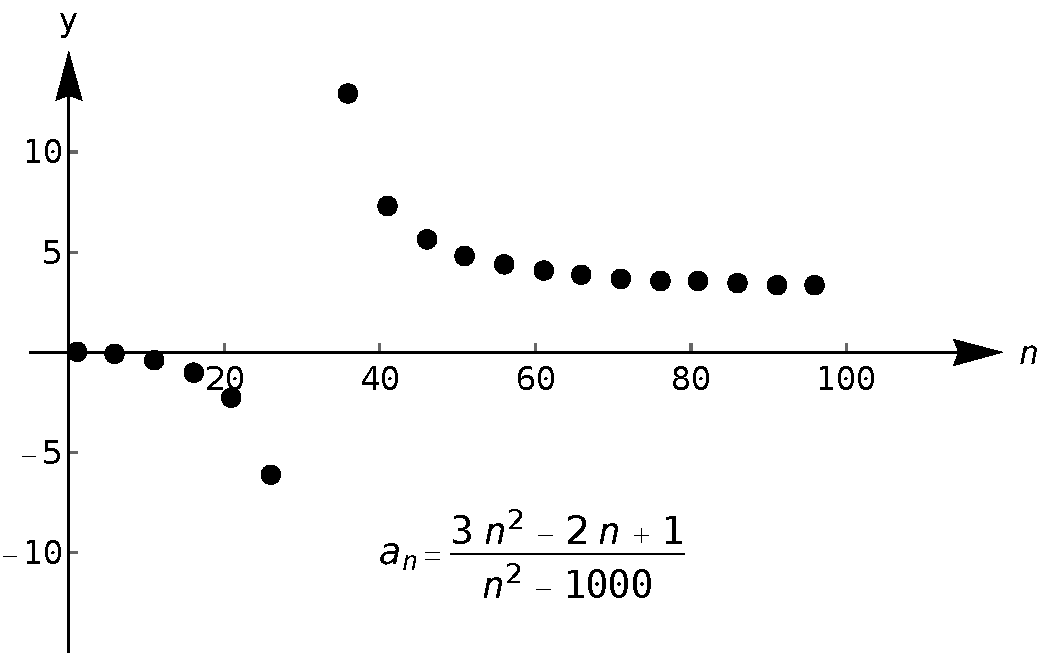
\includegraphics[width=0.45\textwidth]{fig_series_1a}}
\qquad
\subfigure[\label{fig_series_1b}]{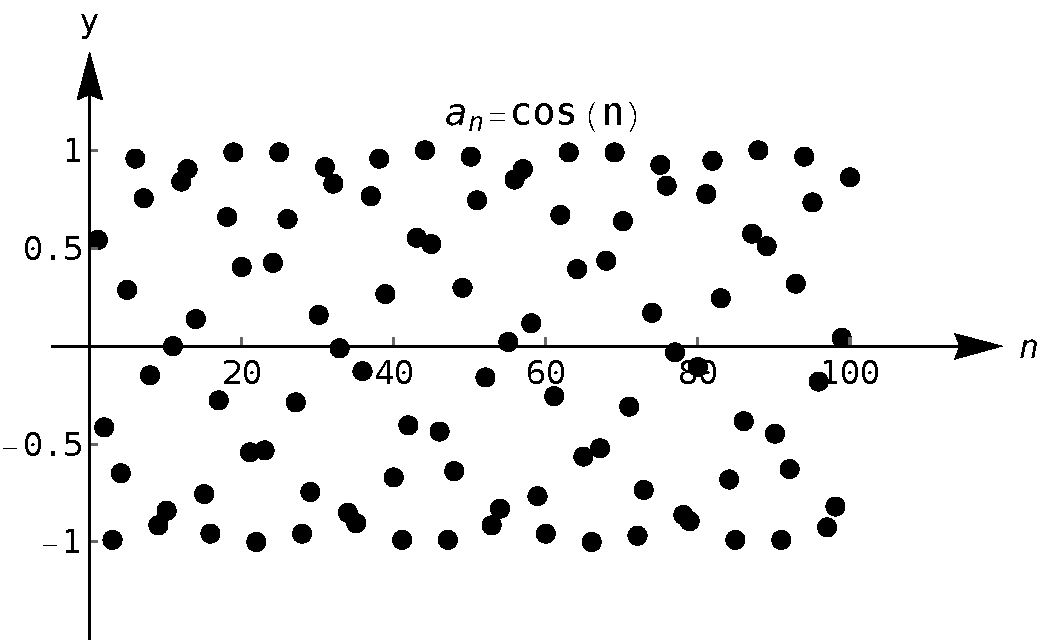
\includegraphics[width=0.45\textwidth]{fig_series_1b} }
\qquad
\subfigure[\label{fig_series_1c}]{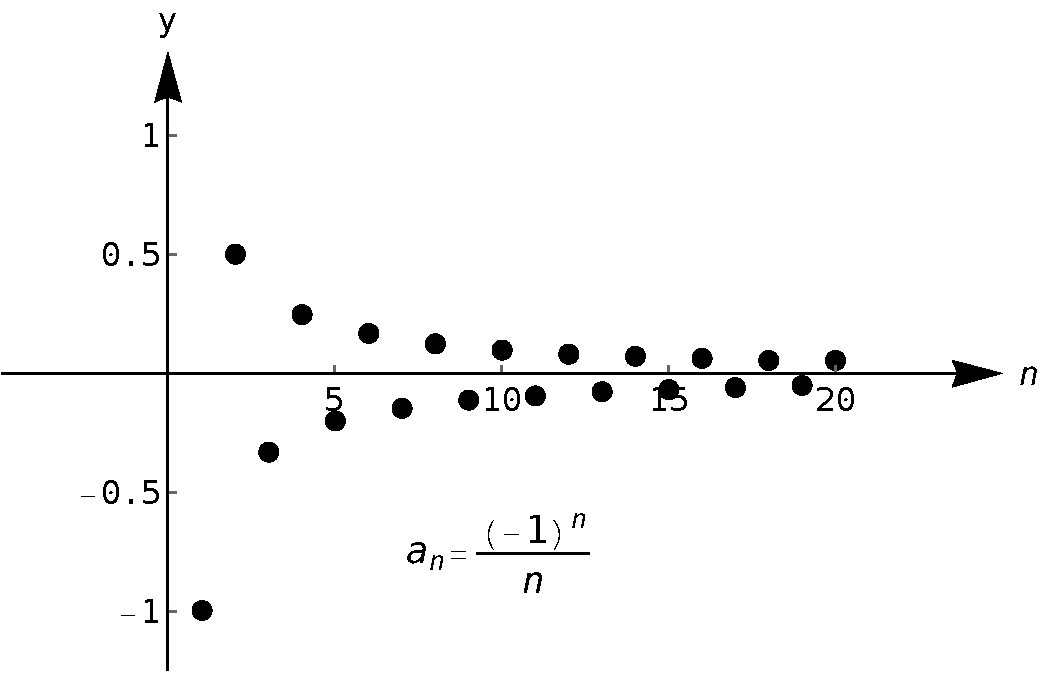
\includegraphics[width=0.45\textwidth]{fig_series_1c} }
\caption{Scatter plots of the sequences in Example \ref{ex_seq4}.}
\end{figure}

In the previous example we used the definition of the limit of a sequence to determine the convergence of a sequence as we could not apply Theorem \ref{thm:seq_limit}. In general, we like to avoid invoking the definition of a limit, and the following theorem gives us tool that we could use in that example instead.


\begin{theorem}[Absolute value theorem]\label{thm:abs_val_seq}
Let $\{a_n\}$ be a sequence. If $\ds \lim_{n\to+\infty} |a_n| = 0$, then $\ds \lim_{n\to+\infty} a_n = 0.$\index{absolute value theorem}\index{limit!absolute value theorem}\index{sequence!absolute value theorem}
\end{theorem}
\ifanalysis

\begin{proof}
The main thing to this proof is to note that
$$
- \left| {{a_n}} \right| \le {a_n} \le \left| {{a_n}} \right|
$$
and
$$
 \ds\lim \limits_{n \to +\infty } \left( { - \left| {{a_n}} \right|} \right) =  -  \lim \limits_{n \to +\infty } \left| {{a_n}} \right| = 0\,.
$$
We then have  $\ds\lim\limits_{n \to +\infty }(-|a_n|)=\lim\limits_{n \to +\infty }(|a_n|)=0$ and so by the squeeze theorem for sequences we must also have that $\ds\lim \limits_{n \to +\infty } {a_n} = 0$.
\end{proof}

\fi
\begin{example}\label{ex_seq5}
Determine the convergence or divergence of the following sequences.
\begin{multicols}{2}
\begin{enumerate}
\item $\ds \{a_n\} = \left\{\frac{(-1)^n}{n}\right\}$ 
\item $\ds \{a_n\} = \left\{\frac{(-1)^n(n+1)}{n}\right\}$ 
\end{enumerate}
\end{multicols}

\xhrulefill{gray}{2.5pt}Solution \xhrulefill{gray}{2.5pt}

\begin{enumerate}
\item		This appeared in Example \ref{ex_seq4}. We want to apply Theorem \ref{thm:abs_val_seq}, so consider the limit of $\{|a_n|\}$:
\begin{align*}
\lim_{n\to+\infty} |a_n| &= \lim_{n\to+\infty} \left|\frac{(-1)^n}{n}\right| \\[0.2cm]
					&= \lim_{n\to+\infty} \frac{1}{n} \\
					&= 0.
\end{align*}
Since this limit is 0, we can apply Theorem \ref{thm:abs_val_seq} and state that $\ds\lim_{n\to+\infty} a_n=0$.

\item Because of the alternating nature of this sequence, we cannot simply look at the limit 
$$\ds \lim_{x\to+\infty} \frac{(-1)^x(x+1)}{x}.$$
We can try to apply the techniques of Theorem \ref{thm:abs_val_seq}:
\begin{align*}
\lim_{n\to+\infty} |a_n| &= \lim_{n\to+\infty} \left|\frac{(-1)^n(n+1)}{n}\right| \\[0.2cm]
							&= \lim_{n\to+\infty} \frac{n+1}{n}=1\,.
							\end{align*}
We have concluded that when we ignore the alternating sign, the sequence approaches 1. This means we cannot apply Theorem \ref{thm:abs_val_seq}; it states the the limit must be 0 in order to conclude anything.

Since we know that the signs of the terms alternate and we know that the limit of $|a_n|$ is 1, we know that as $n$ approaches infinity, the terms will alternate between values close to 1 and $-1$, meaning the sequence diverges. A plot of this sequence is given in Figure \ref{fig_series_2}.
\end{enumerate}

\begin{figure}[H]
	\begin{center}
			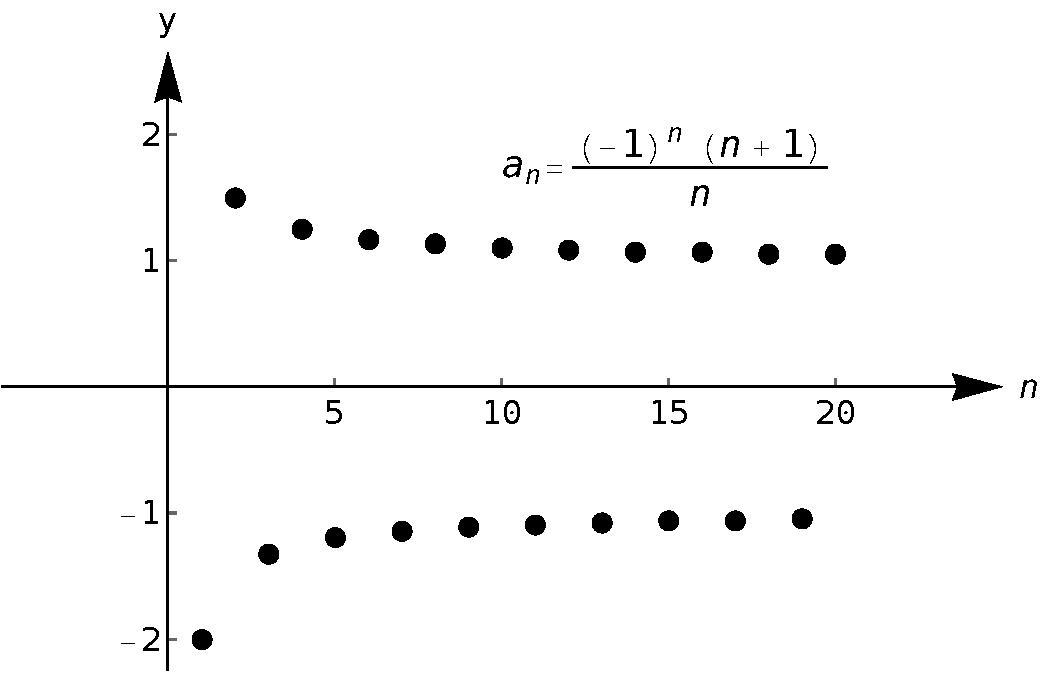
\includegraphics[width=0.5\textwidth]{fig_series_2}
	\caption{A plot of a sequence in Example \ref{ex_seq5}, part 2.}
	\label{fig_series_2}
	\end{center}
\end{figure}


\end{example}

\subsubsection{Properties}
We continue our study of the limits of sequences by considering some of the properties of these limits. These follow easily from the properties of limits of functions discussed in Chapter~\ref{chap_limits}.


Let $\{a_n\}$ and $\{b_n\}$ be sequences such that $\ds \lim_{n\to+\infty} a_n = L$, $\ds \lim_{n\to+\infty} b_n = K$, and let $c$ be a real number. The following properties hold


\begin{enumerate}
\item		$\ds \lim_{n\to+\infty} (a_n\pm b_n) = L\pm K$
\index{sequences!limit properties}
\item		$\ds \lim_{n\to+\infty} (a_n\cdot b_n) = L\cdot K$
\item		$\ds \lim_{n\to+\infty} \left(\dfrac{a_n}{b_n}\right) = \dfrac{L}{K}$, $K\neq 0$
\item		$\ds \lim_{n\to+\infty} c\cdot a_n = c\cdot L$
\end{enumerate}

For instance, let
	$$\ds \{a_n\} = \left\{\frac{n+1}{n^2}\right\},$$
	and
	$$\ds \{b_n\} = \left\{\left(1+\frac1n\right)^{n}\right\},$$
with $\ds \lim_{n\to+\infty} a_n = 0$ and $\ds \lim_{n\to+\infty} b_n = e$, respectively.  Then, $\ds \lim_{n\to+\infty} (a_n+b_n)=e$. Similarly, \\ $\ds \lim_{n\to+\infty} 1000a_n =1000\cdot 0 = 0$. 

\subsubsection{Behaviour}
Let us start with some definitions describing properties of the range of a sequence.

\begin{definition}[Bounded and unbounded sequences]\label{def:bounded}
A sequence $\{a_n\}$ is said to be \textbf{bounded} (\textit{begrensd}) if there exist real numbers $m$ and $M$ such that $m \leq a_n \leq M$ for all $n$ in $\mathbb{N}_0$.\\
A sequence $\{a_n\}$ is said to be \textbf{unbounded} (\textit{onbegrensd}) if it is not bounded.\\
A sequence $\{a_n\}$ is said to be \textbf{bounded above} (\textit{naar boven begrensd}) if there exists an $M$ such that $a_n \leq  M$ for all $n$ in $\mathbb{N}_0$; it is \textbf{bounded below} (\textit{naar beneden begrensd}) if there exists an $m$ such that $m\leq a_n$ for all $n$ in $\mathbb{N}_0$.
\index{sequence!boundedness}\index{bounded sequence}\index{unbounded sequence}\index[aut]{rij ! begrensd}\index[aut]{rij ! onbegrensd}\index[aut]{rij ! naar boven begrends}\index[aut]{rij ! naar beneden begrensd}
\end{definition}

%\enlargethispage{2\baselineskip}
It follows from this definition that an unbounded sequence may be bounded above or bounded below; a sequence that is both bounded above and below is simply a bounded sequence. Alternatively, using absolute values, one may also say that a sequence $\{a_n\}$ is bounded if there exists $M\geq0$ such that $\left|a_n\right|\leq M$ for all $n\in\mathbb{N}_0$. 


\begin{example}\label{ex_seq3}
Determine the boundedness of the following sequences.
\begin{multicols}{2}
\begin{enumerate}
\item $\ds\{a_n\}  = \left\{\frac1n\right\}$ 
\columnbreak
\vspace*{0.01cm}
\item $\{a_n\} = \{2^n\}$ 
\vspace*{0.2cm}
 \end{enumerate}
 \end{multicols}
 
 
\xhrulefill{gray}{2.5pt}Solution \xhrulefill{gray}{2.5pt}

\begin{enumerate}
\item		The terms of this sequence are always positive but are decreasing, so we have $0<a_n<2$ for all $n$. Thus this sequence is bounded. Figure \ref{fig_series_3a} illustrates this.

\item		The terms of this sequence obviously grow without bound. However, it is also true that these terms are all positive, meaning $0<a_n$. Thus we can say the sequence is unbounded, but also bounded below. Figure \ref{fig_series_3b} illustrates this.

\end{enumerate}
\begin{figure}[H]
\centering
%\raisebox{0.5cm}{
\subfigure[\label{fig_series_3a}]{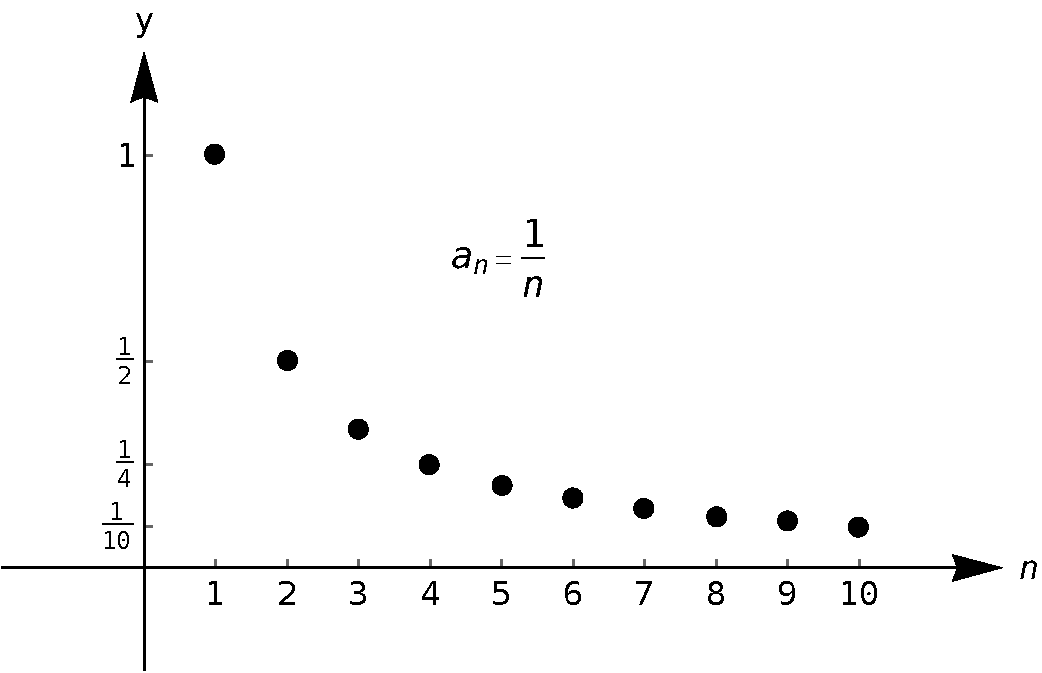
\includegraphics[width=0.45\textwidth]{fig_series_3a}}
\qquad
\subfigure[\label{fig_series_3b}]{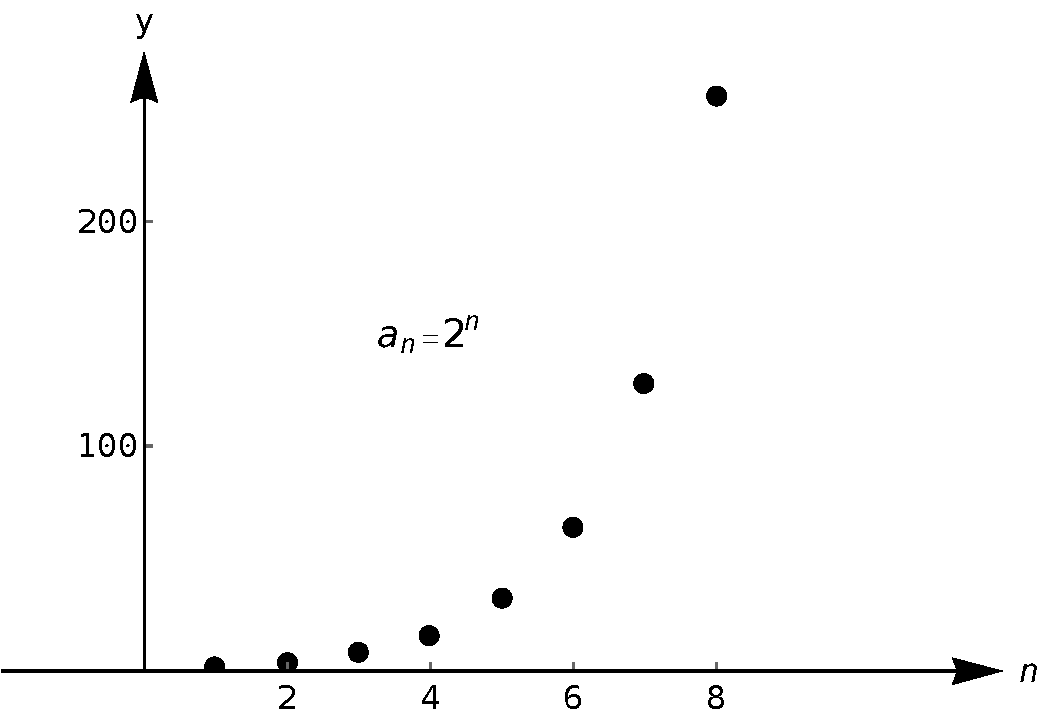
\includegraphics[width=0.45\textwidth]{fig_series_3b} }
\caption{A plot of $\{a_n\} = \{1/n\}$ and $\{a_n\} = \{2^n\}$ from Example \ref{ex_seq3}.}
\end{figure}

\end{example}

The previous example produces some interesting concepts. First, we can recognize that the sequence $\ds\left\{1/n\right\}$ converges to 0. This says, informally, that most of the terms of the sequence are really close to 0. This implies that the sequence is bounded, using the following logic. First, most terms are near 0, so we could find some sort of bound on these terms (using Definition \ref{def:seq_limit}, the bound is $\varepsilon$). That leaves a few terms that are not near 0 (i.e., a finite number of terms). A finite list of numbers is always bounded. 

This logic implies that if a sequence converges, it must be bounded. This is indeed true, as stated by the following theorem.

\begin{theorem}[Convergent sequences are bounded]\label{thm:converge_bounded}
Let $\ds \left\{a_n\right\}$ be a convergent sequence. Then $\{a_n\}$ is bounded.
\index{convergence! sequence}\index{sequence !convergent}\index[aut]{rij ! convergent}
\end{theorem}

Note that this theorem does not say that bounded sequences must converge, nor does it say that if a sequence does not converge, it is not bounded.

\ifanalysis

\begin{proof}
To prove this theorem, let $\left\{a_n\right\}$ be a convergent sequence and let $L=\lim_{n\to+\infty}a_n$. From Definition~\ref{def:seq_limit} with $\varepsilon=1$, there exists an $N\in\mathbb{N}$ such that $\left|a_n-L\right|<1$ whenever $n>N$. Thus for $n>N$ the triangle equality implies that $\left|a_n\right|<1+\left|L\right|$. Now, let $M=\max\left\{\left|a_1\right|,\left|a_2\right|,\ldots,\left|a_N\right|,\left|L\right|+1\right\}$. Then, we have $\left|s_n\right|\leq M$ for all $n\in\mathbb{N}_0$. Consequently, $\left\{a_n\right\}$ is bounded. 
\end{proof}

\fi

We saw already  the sequence $\ds \{b_n\} = \left\{\left(1+1/n\right)^{n}\right\}$, for it was stated that $\ds \lim_{n\to+\infty} b_n = e$. Even though it may be difficult to intuitively grasp the behaviour of this sequence, we now know immediately that it is bounded.

Another interesting concept to come out of Example \ref{ex_seq3} involves the sequence $\{1/n\}$. The terms of the sequence are decreasing. That is, that $a_{n+1} < a_n$ for all $n$. This is easy to show as follows. Clearly $n < n+1$. Taking reciprocals flips the inequality: $1/n > 1/(n+1)$. This is the same as $a_n > a_{n+1}$. Sequences that either steadily increase or decrease are important, so we give this property a name.

\begin{definition}[Monotonic sequence]\label{def:monotonic}
\begin{enumerate}
\item		A sequence $\{a_n\}$ is \textbf{monotonically increasing} (\textit{monotoon stijgend}) if $a_n \leq a_{n+1}$ for all $n$, i.e.,
 $$a_1 \leq a_2 \leq a_3 \leq \cdots\leq a_n \leq a_{n+1} \cdots$$
 \item	A sequence $\{a_n\}$ is \textbf{monotonically decreasing} (\textit{monotoon dalend}) if $a_n \geq a_{n+1}$ for all $n$, i.e.,
 $$a_1 \geq a_2 \geq a_3 \geq \cdots \geq a_n \geq a_{n+1} \cdots$$
 \item	A sequence is \textbf{monotonic} (\textit{monotoon}) if it is monotonically increasing or monotonically decreasing.
\index{sequences!monotonic}\index{monotonic sequence}\index[aut]{rij ! monotoon}\index[aut]{rij ! monotoon dalend}\index[aut]{rij ! monotoon stijgend}
 \end{enumerate}
\end{definition}


It is sometimes useful to call a monotonically increasing sequence strictly increasing if $a_n < a_{n+1}$ for all $n$. A similar statement holds for strictly decreasing.


\begin{example}\label{ex_seq7}
Determine the monotonicity of the following sequences.
\begin{multicols}{2}
\begin{enumerate}
\item $\ds \{a_n\} = \left\{\frac{n+1}n\right\}$
%\item $\ds \{a_n\} = \left\{\frac{n^2-9}{n^2-10n+26}\right\}$
\item $\ds \{a_n\} = \left\{\frac{n^2}{n!}\right\}$	
\end{enumerate}
\end{multicols}
\xhrulefill{gray}{2.5pt}Solution \xhrulefill{gray}{2.5pt}

In each of the following, we will examine $a_{n+1}-a_n$. If $a_{n+1}-a_n \geq 0$, we conclude that $a_n\leq a_{n+1}$ and hence the sequence is increasing. If $a_{n+1}-a_n\leq 0$, we conclude that $a_n\geq a_{n+1}$ and the sequence is decreasing.

\begin{enumerate}
\item	\hfill	$\ds\begin{aligned}[t] a_{n+1}-a_n &= \frac{n+2}{n+1} - \frac{n+1}{n} \\[0.2cm]		
					&= \frac{(n+2)(n)-(n+1)^2}{(n+1)n} \\
					&=	\frac{-1}{n(n+1)}  < 0 \quad\text{ for all $n$.}
				\end{aligned}$ \hfill\null
				
Since $a_{n+1}-a_n<0$ for all $n$, we conclude that the sequence is strictly  decreasing. A scatter plot of this sequence is shown in Figure~\ref{fig_series_4a}. 


%\item		We can clearly see in Figure \ref{fig_series_4b},  that this sequence is not monotonic. However, it does seem that after the first 4 terms it is decreasing. To understand why, consider:

						%\hfill $\ds \begin{aligned}[t]	
						%a_{n+1}-a_n &= \frac{(n+1)^2-9}{(n+1)^2-10(n+1)+26} - \frac{n^2-9}{n^2-10n+26} \\[0.2cm]		
						%		&= \frac{n^2+2n-8}{n^2-8n+17}-\frac{n^2-9}{n^2-10n+26}\\[0.2cm]
						%		&= \frac{(n^2+2n-8)(n^2-10n+26)-(n^2-9)(n^2-8n+17)}{(n^2-8n+17)(n^2-10n+26)}\\[0.2cm]
						%		&= \frac{-10n^2+60n-55}{(n^2-8n+17)(n^2-10n+26)}.\\[0.2cm]
						%		\end{aligned}$\hfill \null		

%We want to know when this is greater than, or less than, 0. The denominator is always positive, therefore we are only concerned with the numerator. For small values of $n$, the numerator is positive. As $n$ grows large, the numerator is dominated by $-10n^2$, meaning the entire fraction will be negative; i.e., for large enough $n$, $a_{n+1}-a_n < 0$. Using the quadratic formula we can determine that the numerator is  negative for $n\geq 5$. In short, the sequence is simply not monotonic, though it is useful to note that for $n\geq 5$, the sequence is monotonically decreasing. 

\item		The plot in Figure \ref{fig_series_4b} shows that the sequence is not monotonic, but it suggests that it is monotonically decreasing after the first term. We perform the usual analysis to confirm this.

					\hfill $\ds \begin{aligned}[t]	
						a_{n+1}-a_n &= \frac{(n+1)^2}{(n+1)!} - \frac{n^2}{n!} \\
								&= \frac{(n+1)^2-n^2(n+1)}{(n+1)!} \\
								&=	\frac{-n^3+2n+1}{(n+1)!}
					\end{aligned}$\hfill \null
					
When $n=1$, the above expression is greater than zero; for $n\geq 2$, the above expression is lower than zero. Thus this sequence is not monotonic, but it is strictly decreasing after the first term.
\end{enumerate}

\begin{figure}[H]
\centering
%\raisebox{0.5cm}{
\subfigure[\label{fig_series_4a}]{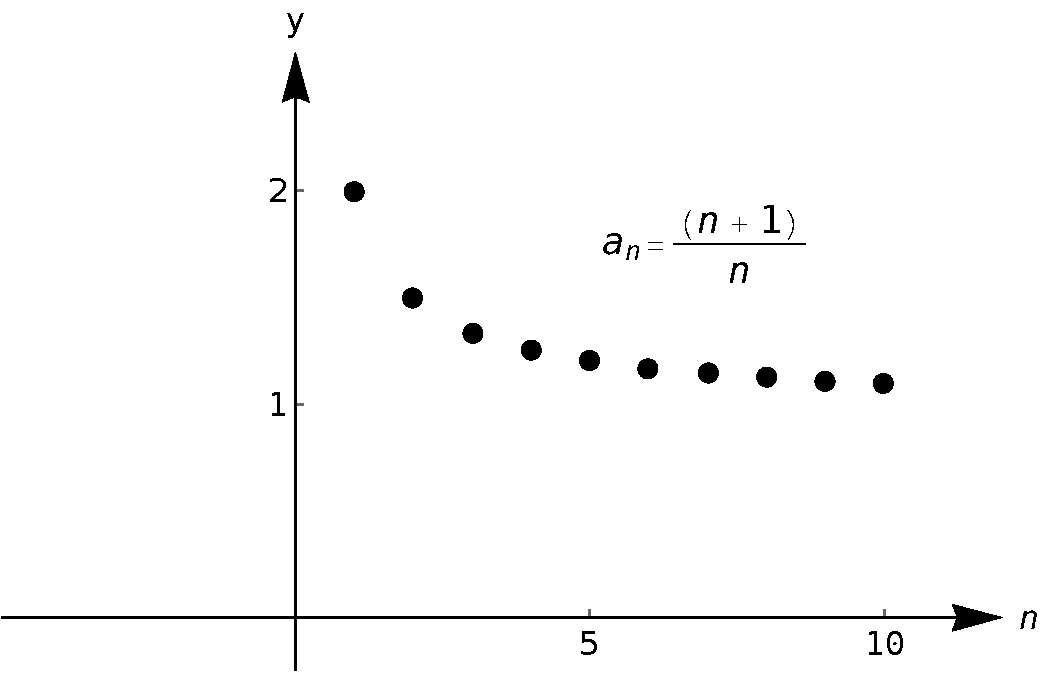
\includegraphics[width=0.45\textwidth]{fig_series_4a}}
\qquad
%\subfigure[\label{fig_series_4b}]{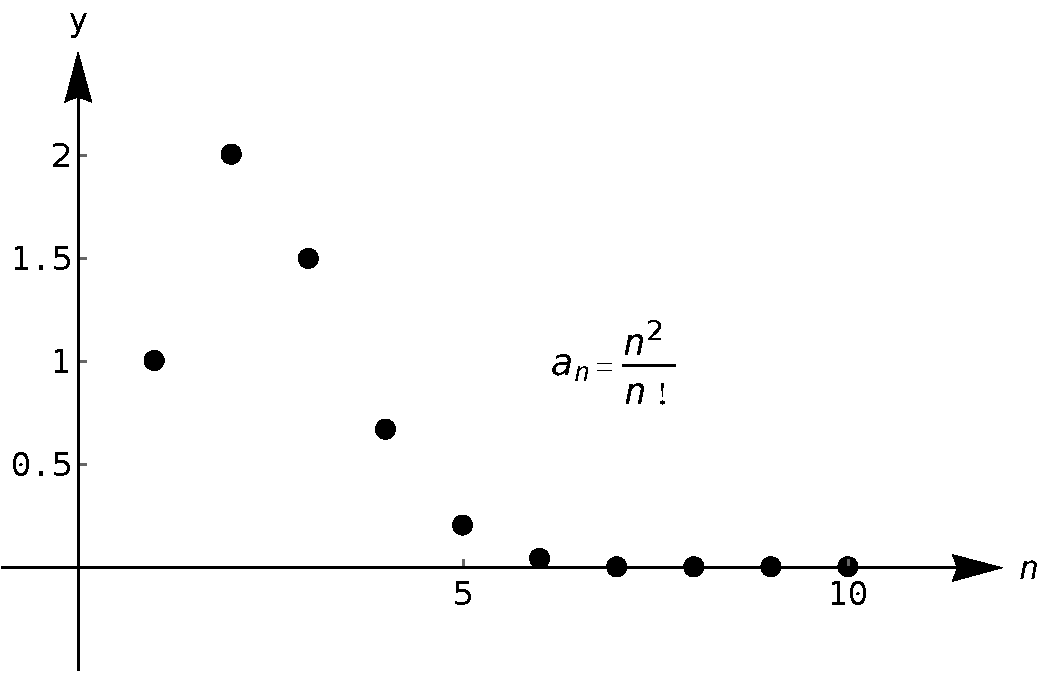
\includegraphics[width=0.45\textwidth]{fig_series_4b} }
%\qquad
\subfigure[\label{fig_series_4b}]{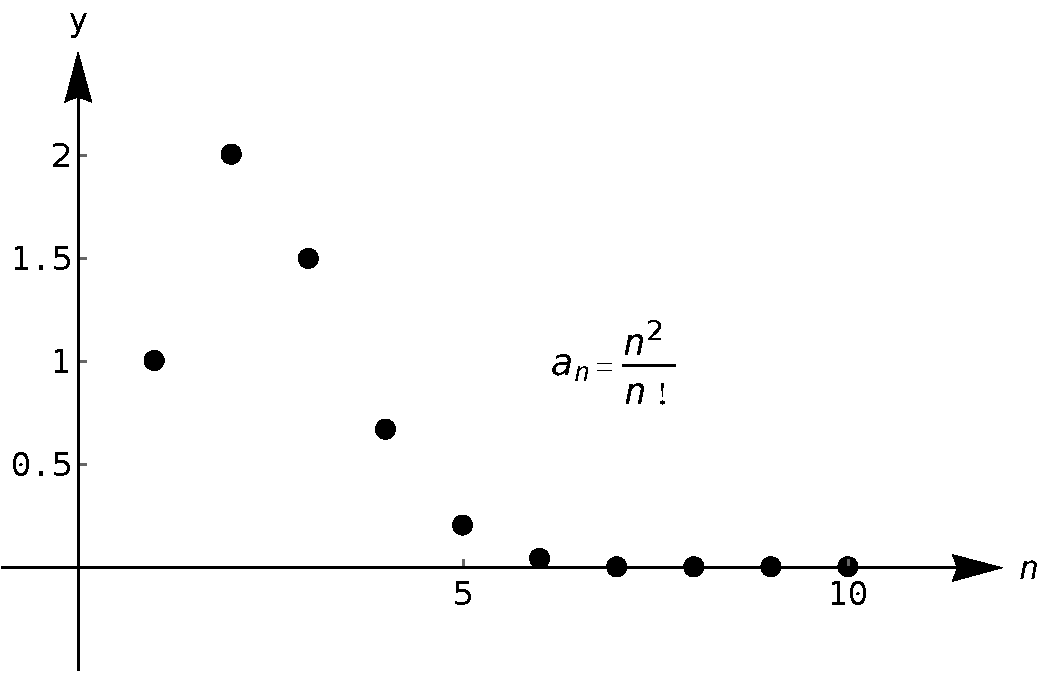
\includegraphics[width=0.45\textwidth]{fig_series_4b} }
\caption{Plots of sequences in Example \ref{ex_seq7}.}
\end{figure}
\end{example}



Knowing that a sequence is monotonic can be useful. Consider, for example, a sequence that is monotonically decreasing and is bounded below. We know the sequence is always getting smaller, but that there is a bound to how small it can become. This is enough to prove that the sequence will converge, as stated in the following theorem.
%\enlargethispage{4\baselineskip}

\begin{theorem}[Monotone convergence theorem]\label{thm:monotonic_converge}
A monotone sequence of real numbers $\left\{a_n\right\}$ converges if and only if it is bounded.
\index{Monotone convergence theorem}
\end{theorem}

\ifanalysis

	\checkoddpage
\marginpar{\ifoddpage\hspace*{-1.5cm}\else\hspace*{0.25cm}\fi
\includegraphics[width=0.075\textwidth]{youtube}\\
\ifoddpage\hspace*{-1.75cm}\else\hspace*{0.1cm}\fi
\qrcode[height=1.75cm]{https://youtu.be/stfRT1If3Ro}
%\includegraphics[width=0.1\textwidth]{monotone_convergentie}
}
\begin{proof}
We already know that a convergent sequence is bounded. Hence we just need to show that a monotone and bounded sequence of real numbers is convergent. Let $\{a_{n}\}$  be such an increasing sequence bounded above. By assumption, $\displaystyle \{a_{n}\}$ is non-empty and bounded above. By the least-upper-bound property of real numbers, the supremum $c=\sup _{n}\{a_{n}\}$ exists and is finite. Now, for every $\varepsilon >0$, $c-\varepsilon$ is not an upper bound. Thus there exists an integer $N$ such that $a_{N}>c-\varepsilon$, 
since otherwise $c-\varepsilon$ is an upper bound of $\{a_{n}\}$, which contradicts to the definition of $c$. Then since $\{a_{n}\}$ is increasing, and $c$ is its upper bound, we have 
$$c-\varepsilon<a_N\leq a_n\leq c<c+\varepsilon $$
or equivalently
$$
\left|a_n-c\right|<\varepsilon
$$
for all $n\geq N$.
Hence, by definition, the limit of $\{a_{n}\}$ is $ \sup _{n}\{a_{n}\}$. 

In the case when the sequence is decreasing, let $c=\inf _{n}\{a_{n}\}$ and proceed in a similar manner.
\end{proof}

\fi

Consider once again the sequence $\{a_n\} = \{1/n\}$. It is easy to show it is monotonically decreasing and that it is always positive (i.e., bounded below by 0). Therefore we can conclude by Theorem \ref{thm:monotonic_converge} that the sequence converges.

Sequences are a great source of mathematical inquiry. The On-Line Encyclopedia of Integer Sequences (OEIS) contains thousands of sequences and their formulae. Perusing this database quickly demonstrates that a single sequence can represent several different real life phenomena. 

Interesting as this is, our interest actually lies elsewhere. We are more interested in the sum of a sequence. That is, given a sequence $\{a_n\}$, we are very interested in $a_1+a_2+a_3+\cdots$. Of course, one might immediately think that thus adds up to infinity?". Many times, yes, but there are many important cases where the answer is no. This is the topic of series, which we begin to investigate in the next section.

\begin{remark}[Fibonacci numbers]
The Fibonacci numbers make up an integer sequence, called the Fibonacci sequence, which is characterized by the fact that every number after the first two is the sum of the two preceding ones:
$$
{\displaystyle 1,\;1,\;2,\;3,\;5,\;8,\;13,\;21,\;34,\;55,\;89,\;144,\;\ldots }
$$
Fibonacci sequences appear in biological settings, such as branching in trees, arrangement of leaves on a stem, the fruitlets of a pineapple, the flowering of artichoke, an uncurling fern and the arrangement of a pine cone, but there are also numerous poorly substantiated claims of Fibonacci numbers, relating to the breeding of rabbits, the seeds on a sunflower, the spirals of shells, and the curve of waves.
\end{remark}

\section{Infinite series}\label{sec:series}
\subsection{Definition}
Given the sequence $\{a_n\} = \{1/2^n\} = 1/2,\ 1/4,\ 1/8,\ \ldots$, consider the following sums:

$$\begin{array}{ccccc}
a_1				&=& 1/2					 &=& 1/2\\
a_1+a_2		&=& 1/2+1/4			 &=& 3/4\\
a_1+a_2+a_3 &=& 1/2+1/4+1/8  &=& 7/8\\
a_1+a_2+a_3+a_4 &=& 1/2+1/4+1/8+1/16 & =& 15/16
\end{array}$$
In general, we can show that $$a_1+a_2+a_3+\cdots +a_n = \frac{2^n-1}{2^n} = 1-\frac{1}{2^n}.$$
Let $S_n$ be the sum of the first $n$ terms of the sequence $\{1/2^n\}$. From the above, we see that $S_1=1/2$, $S_2 = 3/4$, etc. Our formula at the end shows that $S_n = 1-1/2^n$. 

Now consider the following limit: $\ds \lim_{n\to+\infty}S_n = \lim_{n\to+\infty}\big(1-1/2^n\big) = 1$. This limit can be interpreted as saying something amazing: the sum of all the terms of the sequence $\{1/2^n\}$ is 1. This example illustrates some interesting concepts that we explore in this section. We begin this exploration with some definitions.

%\setboxwidth{50pt}
\begin{definition}[Infinite series and partial sums]\label{def:series}
Let $\{a_n\}$ be a sequence.
\begin{enumerate}
\item		The sum $\ds \sum_{n=1}^{+\infty} a_n$ is an \textbf{infinite series} (\textit{oneindige reeks}) (or, simply series).
\item		Let $\ds S_n = \sum_{i=1}^n a_i$\,; the sequence $\{S_n\}$ is the \textbf{sequence of $n^\text{th}$ partial sums of $\{a_n\}$} (\textit{partieelsom}).
\item		If the sequence $\{S_n\}$ converges to $L$, we say the series $\ds \sum_{n=1}^{+\infty} a_n$ \textbf{converges} (\textit{convergeert}) to $L$, and we write $\ds \sum_{n=1}^{+\infty} a_n = L$.
\item		If the sequence $\{S_n\}$ \textbf{diverges} (\textit{divergeert}), the series $\ds \sum_{n=1}^{+\infty} a_n$ diverges.
\index{series!definition}\index{series!partial sums}\index{series!convergent}\index{series!divergent}\index[aut]{reeks ! convergent}
\index[aut]{reeks ! divergent}\index[aut]{reeks ! partieelsom}
\end{enumerate}
\end{definition}



We will explore a variety of series in this section. We start with two series that diverge, showing how we might discern divergence.

\begin{example}\label{ex_series1}
\begin{enumerate}
\item		Let $\{a_n\} = \{n^2\}$. Show $\ds \sum_{n=1}^{+\infty} a_n$ diverges.
\item		Let $\{b_n\} = \{(-1)^{n+1}\}$. Show $\ds \sum_{n=1}^{+\infty} b_n$ diverges.
\end{enumerate}

\xhrulefill{gray}{2.5pt}Solution \xhrulefill{gray}{2.5pt}


\begin{enumerate}
\item	Consider $S_n$, the $n^\text{th}$ partial sum.
\begin{align*} S_n &= a_1+a_2+a_3+\cdots+a_n \\		
						&= 1^2+2^2+3^2\cdots + n^2.
\intertext{By Theorem \ref{thm:summation}, this is}
					S_n &= \frac{n(n+1)(2n+1)}{6}.
\end{align*}
Since $\ds \lim_{n\to+\infty}S_n = +\infty$, we conclude that the series $\ds \sum_{n=1}^{+\infty} n^2$ diverges. It is instructive to write $$\ds \sum_{n=1}^{+\infty} n^2=+\infty$$ for this tells us how the series diverges: it grows without bound. A scatter plot of the sequences $\{a_n\}$ and $\{S_n\}$ is given in Figure \ref{fig_series_5a}. The terms of $\{a_n\}$ are growing, so the terms of the partial sums $\{S_n\}$ are growing even faster, illustrating that the series diverges.

%\mfigure{.5}{Scatter plots relating to the series of Example \ref{ex_series1} part 1.}{fig:series1a}{figures/figseries1a}

\item		The sequence $\{b_n\}$ starts with 1, $-1$, 1, $-1$, $\ldots$. Consider some of the partial sums $S_n$ of $\{b_n\}$:
\begin{align*}
S_1 &= 1\\
S_2 &= 0\\
S_3 &= 1\\
S_4 &= 0
\end{align*}
This pattern repeats; we find that $S_n = 1$ if $n$ is odd and $S_n=0$ if $n$ is even. As $\{S_n\}$ oscillates, repeating 1, 0, 1, 0, $\ldots$, we conclude that $\ds\lim_{n\to+\infty}S_n$ does not exist, hence the series under study diverges.	A scatter plot of the sequence $\{b_n\}$ and the partial sums $\{S_n\}$ is given in Figure \ref{fig_series_5b}. When $n$ is odd, $b_n = S_n$ so the marks for $b_n$ are drawn oversized to show they coincide.	
																			
\end{enumerate}

\begin{figure}[H]
\centering
%\raisebox{0.5cm}{
\subfigure[\label{fig_series_5a}]{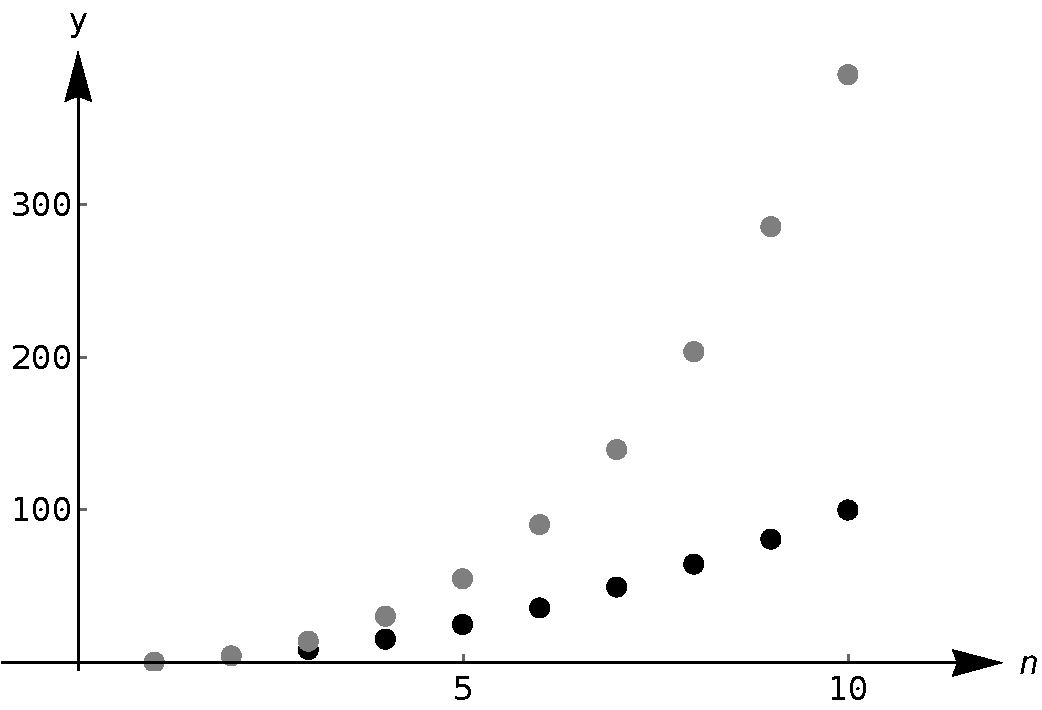
\includegraphics[width=0.45\textwidth]{fig_series_5a}}
\qquad
\subfigure[\label{fig_series_5b}]{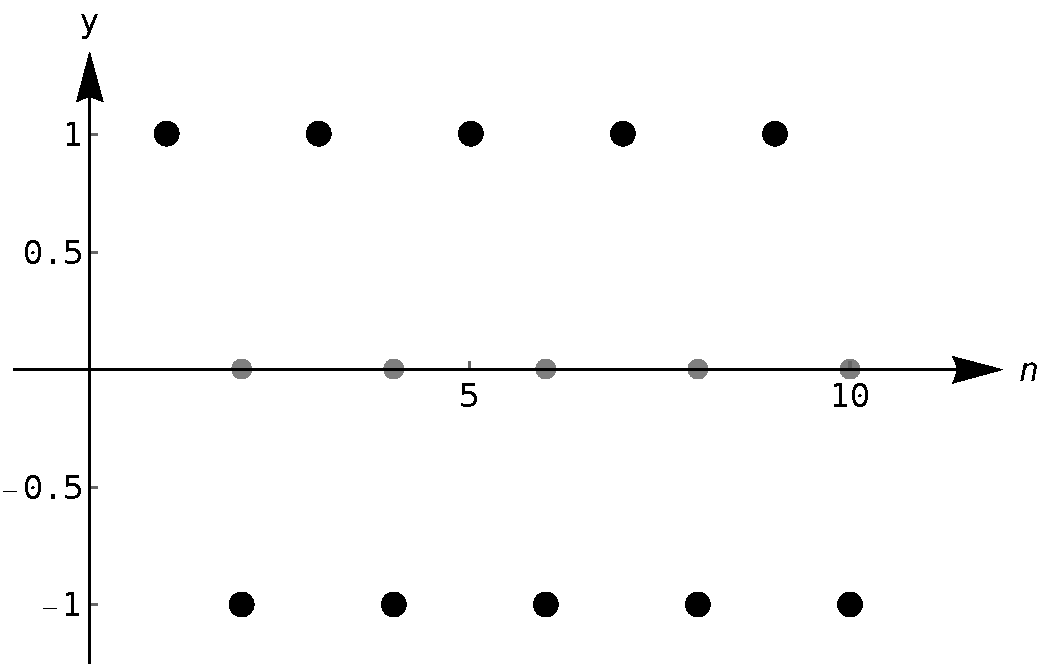
\includegraphics[width=0.45\textwidth]{fig_series_5b} }
\caption{Scatter plots of $a_n$ (black) and $S_n$ (grey) relating to Example \ref{ex_series1}.}
\end{figure}

\end{example}

While it is important to recognize when a series diverges, we are generally more interested in series that  converge. In this section we will only demonstrate a few general techniques for determining convergence; later sections will delve deeper into this topic. 


\subsection{Geometric and $p$-series}
One important type of series is a geometric series.

\begin{definition}[Geometric series]\label{def:geom_series}
A \textbf{geometric series} (\textit{meetkundige reeks}) is a series of the form 
$$\sum_{n=0}^{+\infty} r^n = 1+r+r^2+r^3+\cdots+r^n+\cdots$$
Note that the index starts at $n=0$, not $n=1$.%
\index{series!geometric}\index{geometric series}\index[aut]{reeks ! meetkundige}\index[aut]{meetkundige reeeks}
\end{definition}

 One reason geometric series are important is that they have nice convergence properties, as stated in the following theorem

\begin{theorem}[Geometric series test]\label{thm:geom_series}
Consider the geometric series $$\ds \sum_{n=0}^{+\infty} r^n.$$
\begin{enumerate}
\item		The $n^\text{th}$ partial sum is: $\ds S_n = \frac{1-r\,^{n}}{1-r}$, $r\neq 1$.
\item		The series converges if and only if $|r| < 1$. When $|r|<1$, 
\index{series!geometric}\index{geometric series}\index{convergence!of geometric series}\index{divergence!of geometric series}
$$\sum_{n=0}^{+\infty} r^n = \frac{1}{1-r}.$$
\end{enumerate}
\end{theorem}

\ifanalysis

\begin{proof}
Let us first of all construct the formula for the $n$-th partial sum. For $r\neq 1$, the sum of the first $n$ terms of a geometric series is 
$$
\displaystyle{\begin{array}{rrcl}
& S_n & =& 1+r+r^{2}+r^{3}+\cdots+r^{n-1},\\
\Rightarrow & rS_n & = & r+r^{2}+r^{3}+r^{4}+\cdots +r^{n},\\
\Rightarrow & S_n-rS_n & = & 1-r^{n},\\
\Rightarrow &  S_n(1-r)& = &1-r^{n},\end{array} }
$$
so,
$$
\displaystyle S_n=\frac {1-r^{n}}{1-r}
$$
if $r\neq 1$.

Clearly, as $n$ goes to infinity, the absolute value of $r$ must be less than one for the series to converge. The sum then becomes
$$
1+r+r^{2}+r^{3}+r^{4}+\cdots =\sum _{n=0}^{+\infty }r^{n}={\frac {a}{1-r}}\,,
$$
for $\left|r\right|<1$	because $\lim\limits_{n\to+\infty} r^n=0$ for $\left|r\right|<1$. 
\end{proof}

\fi

According to Theorem \ref{thm:geom_series}, the series of the introductory example, i.e.
$$\ds\sum_{n=0}^{+\infty} \frac{1}{2^n} =\sum_{n=0}^{+\infty} \left(\frac 12\right)^n= 1+\frac12+\frac14+\cdots$$ converges as $r=1/2$, and $$\ds \sum_{n=0}^{+\infty} \frac{1}{2^n} = \frac{1}{1-1/2} = 2.$$ This concurs with our findings in the introductory example; while there we got a sum of 1, we skipped the first term of 1.

\begin{example}\label{ex_series2}
Check the convergence of 
$$\ds \sum_{n=2}^{+\infty} \left(\frac34\right)^n\,.$$
 If it converges, find its sum.


\xhrulefill{gray}{2.5pt}Solution \xhrulefill{gray}{2.5pt}


Since $r=3/4<1$, this series converges. By Theorem \ref{thm:geom_series}, we have that
$$\sum_{n=0}^{+\infty} \left(\frac34\right)^n = \frac{1}{1-3/4} = 4.$$ However, note the subscript of the summation in the given series: we are to start with $n=2$. Therefore we subtract the first two terms, giving:
$$\sum_{n=2}^{+\infty} \left(\frac34\right)^n = 4 - 1 - \frac34 = \frac94.$$
This is illustrated in Figure \ref{fig_series_6}.


\begin{figure}[H]
	\begin{center}
			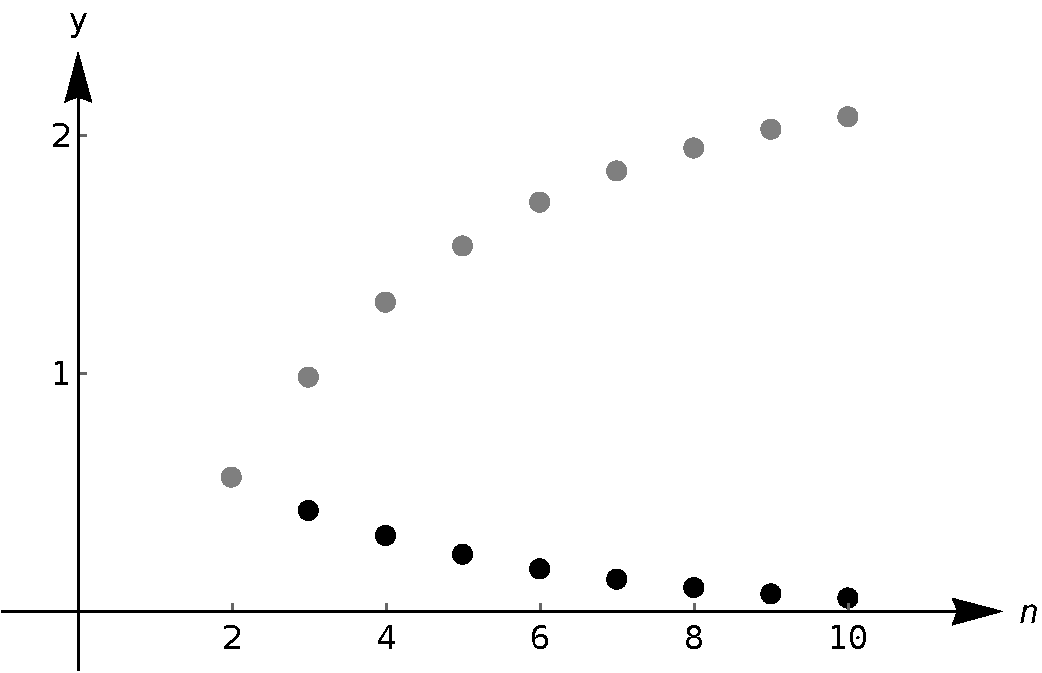
\includegraphics[width=0.5\textwidth]{fig_series_6}
	\caption{Scatter plots of $a_n$ (black) and $S_n$ (gray) relating to the series in Example \ref{ex_series2}.}
	\label{fig_series_6}
	\end{center}
\end{figure}
\end{example}

Another important type of series is the p-series.

\begin{definition}[$p$-series]\label{def:pseries}
\begin{enumerate}
\item	A \textbf{$p$--series} (\textit{$p$-reeks}) is a series of the form $$\sum_{n=1}^{+\infty} \frac{1}{n^p},$$\\
\qquad \text{where $p>0$.}

\item	A \textbf{general $p$--series} is a series of the form 
\index{series!p@$p$-series}\index{p@$p$-series}
$$\sum_{n=1}^{+\infty} \frac{1}{(an+b)^p},$$\\
\qquad \text{where $p>0$ and $a$, $b$ are real numbers.}
\end{enumerate}
\end{definition}
\index{$p$--series}\index[aut]{reeks ! harmonische}\index[aut]{harmonische reeks}

Like geometric series, one of the nice things about $p$--series is that they have easy to determine convergence properties.



\begin{theorem}[$p$--series test]\label{thm:pseries}
A general $p$--series 
$$\ds\sum_{n=1}^{+\infty} \frac{1}{(an+b)^p}$$
 will converge if, and only if, $p>1$.
\end{theorem}
Note that Theorem \ref{thm:pseries} assumes that $an+b\neq 0$ for all $n$. If $an+b=0$ for some $n$, then of course the series does not converge regardless of $p$ as not all of the terms of the sequence are defined. This can be proofed using the integral test (Theorem~\ref{thm:integral_test}), which we will introduce in the next section. 


\begin{example}\label{ex_series6}
Determine the convergence of the following series.\\
\begin{multicols}{4}
\begin{enumerate}
\item		$\ds\sum_{n=1}^{+\infty} \frac{1}{n}$
\item		$\ds\sum_{n=1}^{+\infty} \frac{1}{n^2}$
\item		$\ds\sum_{n=1}^{+\infty} \frac{1}{\sqrt{n}}$
\item		$\ds\sum_{n=1}^{+\infty} \frac{(-1)^n}{n}$
\end{enumerate}
\end{multicols}

\xhrulefill{gray}{2.5pt}Solution \xhrulefill{gray}{2.5pt}


\begin{enumerate}
\item		This is a $p$--series with $p=1$. By Theorem \ref{thm:pseries}, this series diverges. 

This series is a famous series, called the \textbf{harmonic series} (\textit{harmonische reeks}), so named because of its relationship to harmonics in the study of music and sound. \index{harmonic series} \index[aut]{reeks ! harmonische}\index[aut]{harmonische reeks}

\item		This is a $p$--series with $p=2$. By Theorem \ref{thm:pseries}, it converges. Note that the theorem does not give a formula by which we can determine what the series converges to; we just know it converges. A famous, unexpected result is that this series converges to $\ds{\pi^2}/{6}$.

\item		This is a $p$--series with $p=1/2$; the theorem states that it diverges.

\item		This is not a $p$--series, it is a so-called \textbf{alternating harmonic series} (\textit{alternerende harmonische reeks}); the definition does not allow for alternating signs. Therefore we cannot apply Theorem \ref{thm:pseries}. Another famous result states that it  converges to $\ln(2)$. \index{alternating harmonic series} \index[aut]{reeks ! alternerende harmonische}\index[aut]{alternerende harmonische reeks}

\end{enumerate}
\end{example}

\ifanalysis

Later sections will provide tests by which we can determine whether or not a given series converges. This, in general, is much easier than determining what a given series converges to. There are many cases, though, where the sum can be determined. 


\begin{example}\label{ex_series3}
Evaluate the sum

$$
\ds \sum_{n=1}^{+\infty} \left(\frac1n-\frac1{n+1}\right).$$

\index{series!telescoping}\index{telescoping series}


It will help to write down some of the first few partial sums of this series.
\begin{align*}
S_1 &=	\frac11-\frac12 & & = 1-\frac12\\
S_2 &=	\left(\frac11-\frac12\right) + \left(\frac12-\frac13\right) & & = 1-\frac13\\
S_3 &=	\left(\frac11-\frac12\right) + \left(\frac12-\frac13\right)+\left(\frac13-\frac14\right) & &= 1-\frac14\\
S_4 &=	\left(\frac11-\frac12\right) + \left(\frac12-\frac13\right)+\left(\frac13-\frac14\right) +\left(\frac14-\frac15\right)& &= 1-\frac15
\end{align*}
Note how most of the terms in each partial sum are cancelled out! In general, we see that $\ds S_n = 1-\frac{1}{n+1}$. The sequence $\{S_n\}$ converges,  as $\ds \lim_{n\to+\infty}S_n = \lim_{n\to+\infty}\left(1-\frac1{n+1}\right) = 1$, and so we conclude that $$\ds \sum_{n=1}^{+\infty} \left(\frac1n-\frac1{n+1}\right) = 1.$$ Partial sums of the series are plotted in Figure \ref{fig_series_7}.

\begin{figure}[H]
	\begin{center}
			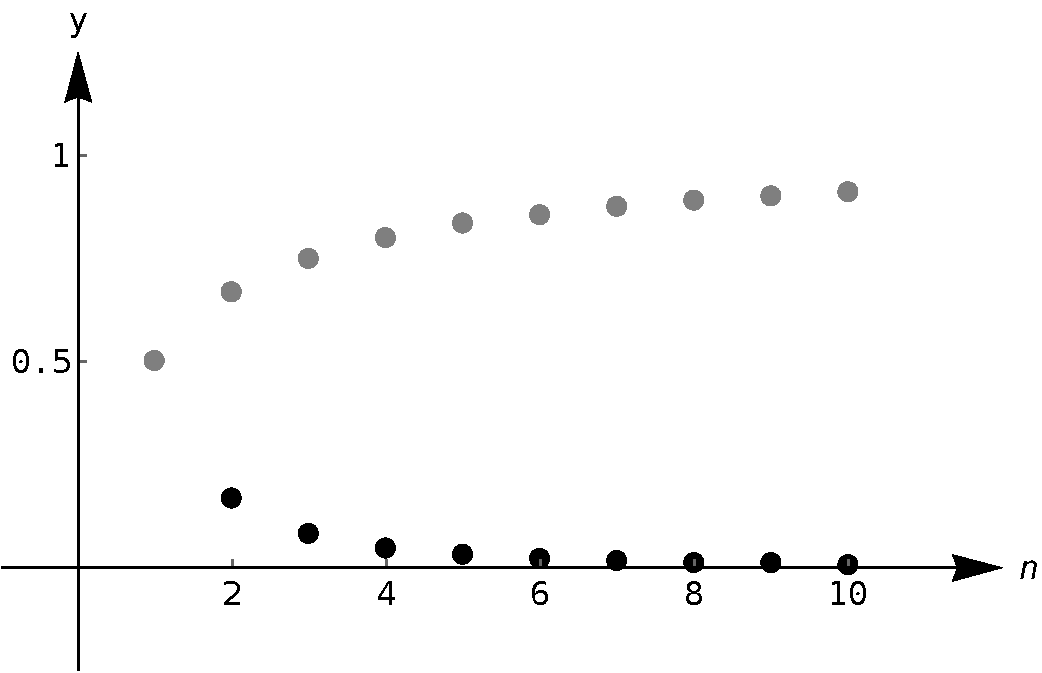
\includegraphics[width=0.5\textwidth]{fig_series_7}
	\caption{Scatter plots of $a_n$ (black) and $S_n$ (gray) relating to the series of Example \ref{ex_series3}.}
	\label{fig_series_7}
	\end{center}
\end{figure}


\end{example}

The series in Example \ref{ex_series3} is an example of a telescoping series. Informally, a telescoping series is one in which most terms cancel with preceding or following terms, reducing the number of terms in each partial sum. The partial sum $S_n$ did not contain $n$ terms, but rather just two: 1 and $1/(n+1)$.\index{series!telescoping}\index{telescoping series}

When possible, seek a way to write an explicit formula for the $n^\text{th}$ partial sum $S_n$. This makes evaluating the limit $\ds\lim_{n\to+\infty} S_n$ much more approachable. We do so in the next example.


\fi


\ifcalculus
Later sections will provide tests by which we can determine whether or not a given series converges. This, in general, is much easier than determining what a given series converges to. There are many cases, though, where the sum can be determined. When possible, seek a way to write an explicit formula for the $n^\text{th}$ partial sum $S_n$. This makes evaluating the limit $\ds\lim_{n\to+\infty} S_n$ much more approachable. We do so in the next example.
\fi



\begin{example}\label{ex_series4}
Evaluate each of the following infinite series.
\begin{multicols}{2}
\begin{enumerate}
\item$\ds \sum_{n=1}^{+\infty}\frac{2}{n^2+2n}$ 
\item $\ds \sum_{n=1}^{+\infty} \ln\left(\frac{n+1}{n}\right)$
\end{enumerate}
\end{multicols}

\xhrulefill{gray}{2.5pt}Solution \xhrulefill{gray}{2.5pt}

\begin{enumerate}
\item		We can decompose the general term as $$\frac2{n^2+2n} = \frac1n-\frac1{n+2}.$$ (See Section \ref{sec:partial_fraction})

Expressing the terms of $\{S_n\}$ is now more instructive.
\begin{align*}
S_1 &= 1-\frac13 &= 1-\frac13\\
S_2 &= \left(1-\frac13\right) + \left(\frac12-\frac14\right) &= 1+\frac12-\frac13-\frac14\\
S_3 &= \left(1-\frac13\right) + \left(\frac12-\frac14\right)+\left(\frac13-\frac15\right) &= 1+\frac12-\frac14-\frac15\\
S_4 &= \left(1-\frac13\right) + \left(\frac12-\frac14\right)+\left(\frac13-\frac15\right)+\left(\frac14-\frac16\right) &= 1+\frac12-\frac15-\frac16\\
\end{align*}
\normalsize


\ifanalysis We again have a telescoping series. \fi In each partial sum, most of the terms cancel and we obtain the formula
$$\ds S_n = 1+\frac12-\frac1{n+1}-\frac1{n+2}.$$
Taking limits allows us to determine the convergence of the series:
$$\lim_{n\to+\infty}S_n = \lim_{n\to+\infty} \left(1+\frac12-\frac1{n+1}-\frac1{n+2}\right) = \frac32,$$
so
$$
\sum_{n=1}^{+\infty} \frac1{n^2+2n} = \frac32.$$

This is illustrated in Figure \ref{fig_series_8a}.

\item		We begin by writing the first few partial sums of the series.

\begin{align*}
S_1 &= \ln\left(2\right) \\
S_2 &= \ln\left(2\right)+\ln\left(\frac32\right) \\
S_3 &= \ln\left(2\right)+\ln\left(\frac32\right)+\ln\left(\frac43\right) \\
S_4 &= \ln\left(2\right)+\ln\left(\frac32\right)+\ln\left(\frac43\right)+\ln\left(\frac54\right) 
\end{align*}
At first, this does not seem helpful, but recall the logarithmic identity: $\ln (x)+\ln (y) = \ln (xy).$ Applying this to $S_4$ gives:
$$S_4 = \ln\left(2\right)+\ln\left(\frac32\right)+\ln\left(\frac43\right)+\ln\left(\frac54\right) = \ln\left(\frac21\cdot\frac32\cdot\frac43\cdot\frac54\right) = \ln\left(5\right).$$

We can conclude that $\{S_n\} = \big\{\ln (n+1)\big\}$. This sequence  does not converge, as \\ $\ds \lim_{n\to+\infty}S_n=+\infty$. Therefore, we have that  
$$\ds\sum_{n=1}^{+\infty}  \ln\left(\frac{n+1}{n}\right)=+\infty,$$ which indicates that
 the series diverges. Note in Figure \ref{fig_series_8b} how the sequence of partial sums grows slowly; after 100 terms, it is not yet over 5. Graphically we may be fooled into thinking the series converges, but our analysis above shows that it does not.
%\mfigure{.35}{Scatter plots relating to the series of Example \ref{ex_series4} part 2.}{fig:series4b}{figures/figseries4b}
\end{enumerate}
\begin{figure}[H]
\centering
%\raisebox{0.5cm}{
\subfigure[\label{fig_series_8a}]{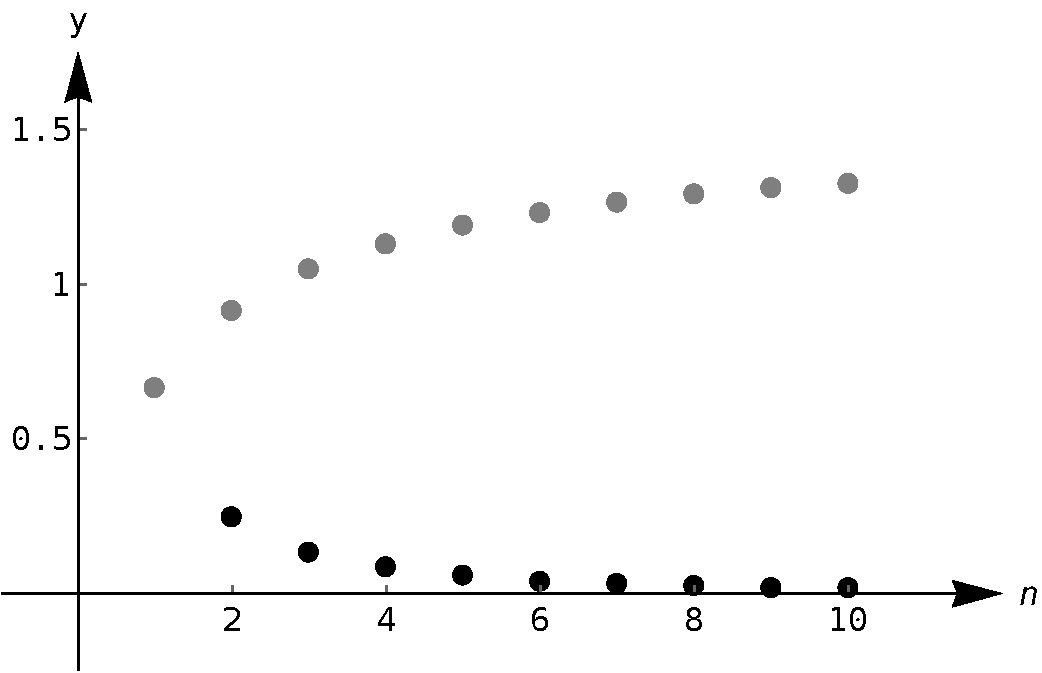
\includegraphics[width=0.45\textwidth]{fig_series_8a}}
\qquad
\subfigure[\label{fig_series_8b}]{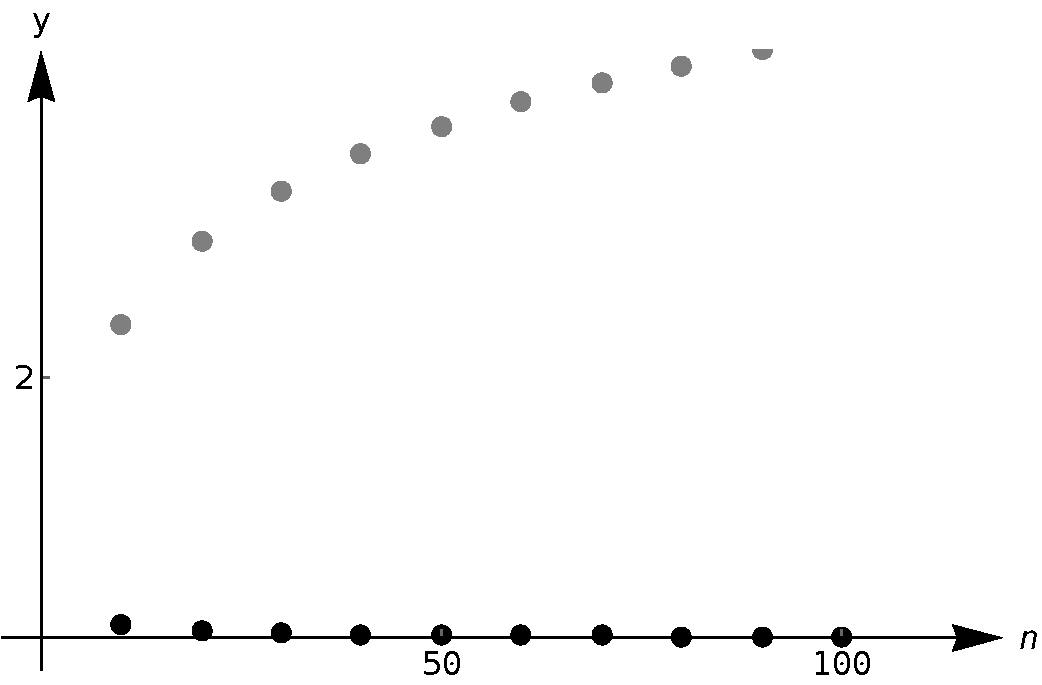
\includegraphics[width=0.45\textwidth]{fig_series_8b} }
\caption{Scatter plots of $a_n$ and $S_n$ relating to Example \ref{ex_series4}.}
\end{figure}

\end{example}

In addition to the geometric, $p$-, harmonic and alternating harmonic series, there are a few more famous series that we will encounter from time to time later on. They are listed below for comprehenseveness.
\begin{equation}
    \ds\sum_{n=0}^{+\infty} \frac1{n!} = e\end{equation}
\begin{equation}\ds\sum_{n=1}^{+\infty} \frac1{n^2} = \frac{\pi^2}{6}\end{equation}
\begin{equation}\ds\sum_{n=1}^{+\infty} \frac{(-1)^{n+1}}{n^2} = \frac{\pi^2}{12}\end{equation}
\begin{equation}\ds\sum_{n=0}^{+\infty} \frac{(-1)^{n}}{2n+1} = \frac{\pi}{4}\end{equation}



\subsection{Properties}

Let \quad$\ds \sum_{n=1}^{+\infty} a_n = L$,\quad  $\ds\sum_{n=1}^{+\infty} b_n = K$, and let $c$ be a constant. Then, the following properties follow easily after some algebra. 
\begin{enumerate}
\item  Constant multiple rule: 
$$\ds\sum_{n=1}^{+\infty} c\cdot a_n = c\cdot\sum_{n=1}^{+\infty} a_n = c\cdot L.$$
\item		Sum/difference rule: 
$$\ds\sum_{n=1}^{+\infty} \big(a_n\pm b_n\big) = \sum_{n=1}^{+\infty} a_n \pm \sum_{n=1}^{+\infty} b_n = L \pm K.$$
\end{enumerate} 

\begin{example}\label{ex_series5}
Evaluate the given series.
\begin{multicols}{2}
\begin{enumerate}
\item $\ds\sum_{n=1}^{+\infty} \frac{(-1)^{n+1}\big(n^2-n\big)}{n^3}$
\item $\ds\sum_{n=1}^{+\infty} \frac{1000}{n!}$
\end{enumerate}
\end{multicols}

\xhrulefill{gray}{2.5pt}Solution \xhrulefill{gray}{2.5pt}

\begin{enumerate}
\item	We start by using algebra to break the series apart:
\begin{align*}
\sum_{n=1}^{+\infty} \frac{(-1)^{n+1}\big(n^2-n\big)}{n^3} &= \sum_{n=1}^{+\infty}\left(\frac{(-1)^{n+1}n^2}{n^3}-\frac{(-1)^{n+1}n}{n^3}\right) \\[0.2cm]
						&= \sum_{n=1}^{+\infty}\frac{(-1)^{n+1}}{n}-\sum_{n=1}^{+\infty}\frac{(-1)^{n+1}}{n^2} \\[0.2cm]
						&= \ln(2) - \frac{\pi^2}{12}	\approx	-0.1293.\\[0.2cm]
\end{align*}
This is illustrated in Figure \ref{fig_series_9a}.
%\mfigure{.75}{Scatter plots relating to the series of Example \ref{ex_series5} part 1.}{fig:series5a}{figures/figseries5a}

\item		This looks very similar to the series that involves $e$ in the list above. Note, however, that the series given in this example starts with $n=1$ and not $n=0$. The first term of the series in the list above is $1/0! = 1$, so we will subtract this from our result below:
\begin{align*}
		\sum_{n=1}^{+\infty} \frac{1000}{n!} &= 1000\cdot\sum_{n=1}^{+\infty} \frac{1}{n!} \\
							&= 1000\cdot (e-1) \approx  1718.28.
\end{align*}
This is illustrated in Figure \ref{fig_series_9b}. The graph shows how this particular series converges very rapidly.
%\mfigure{.45}{Scatter plots relating to the series of Example \ref{ex_series5} part 2.}{fig:series5b}{figures/figseries5b}

\end{enumerate}
\begin{figure}[H]
\centering
%\raisebox{0.5cm}{
\subfigure[\label{fig_series_9a}]{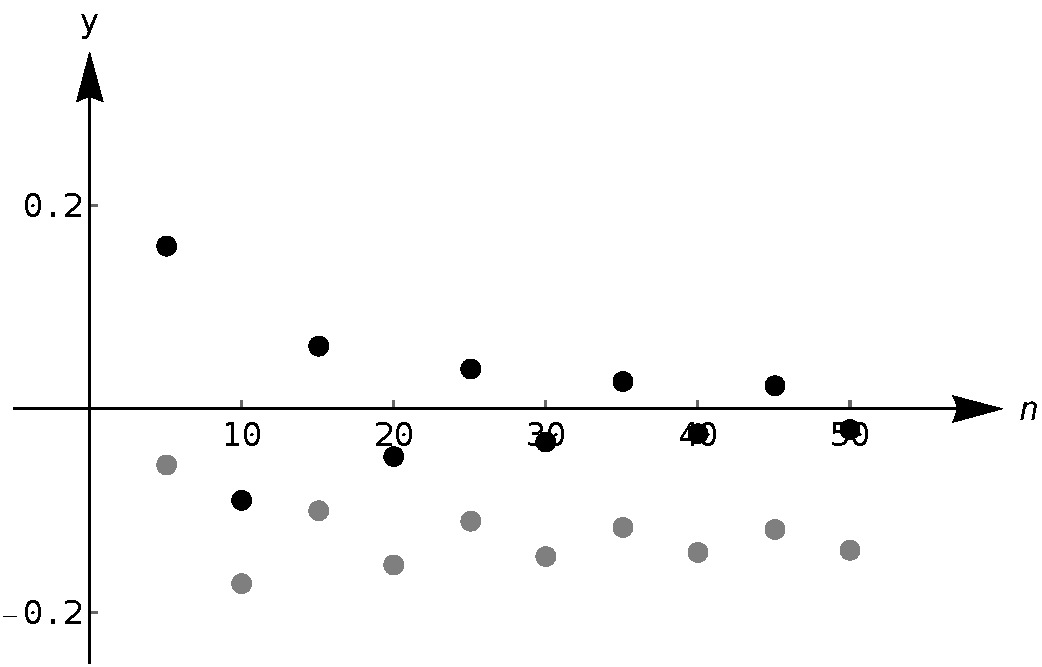
\includegraphics[width=0.45\textwidth]{fig_series_9a}}
\qquad
\subfigure[\label{fig_series_9b}]{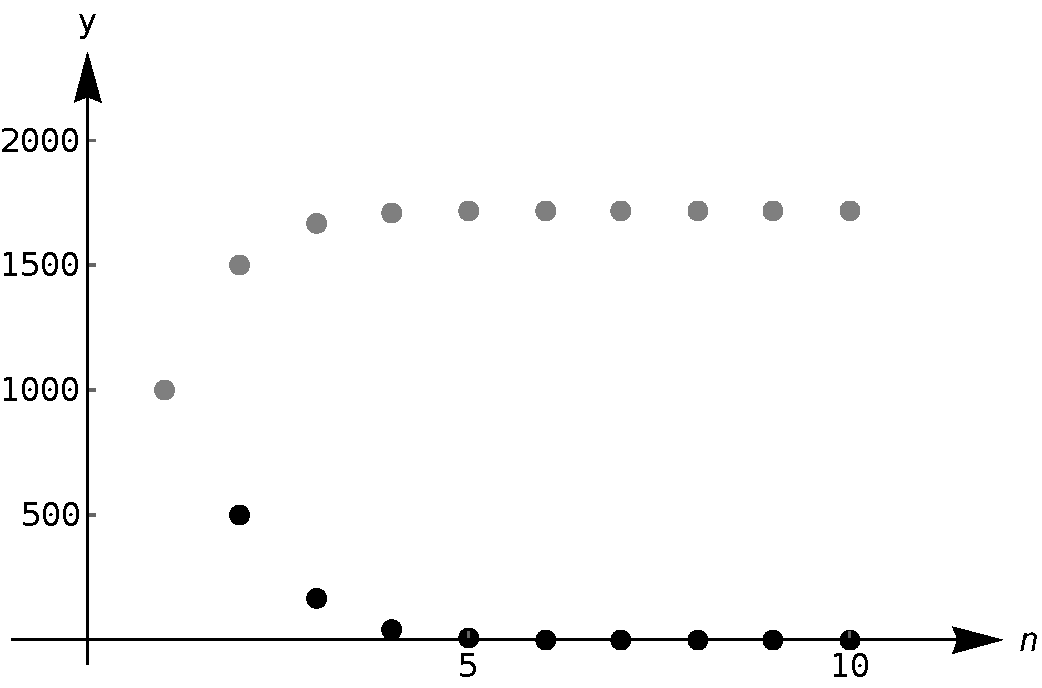
\includegraphics[width=0.45\textwidth]{fig_series_9b} }
\caption{Scatter plots of $a_n$ (black) and $S_n$ (gray) relating to Example \ref{ex_series5}.}
\end{figure}
\end{example}

\subsection{Divergence test}
As one contemplates the behavior of series, a few facts become clear. 
\begin{enumerate}
\item		In order to add an infinite list of nonzero numbers and get a finite result, most of those numbers must be very near 0. 
\item		If a series diverges, it means that the sum of an infinite list of numbers is not finite (it may approach $\pm \infty$ or it may oscillate), and:
		\begin{enumerate}
		\item		The series will still diverge if the first term is removed.
		\item		The series will still diverge if the first 10 terms are removed.
		\item		The series will still diverge if the first $1000000$ terms are removed.
		\item		The series will still diverge if any finite number of terms from anywhere in the series are removed.
		\end{enumerate}
\end{enumerate}

These concepts are very important and lie at the heart of the next two theorems.

\begin{theorem}[$n^\text{th}$--term test for divergence]\label{thm:series_nth_term}
Consider the series $$\ds\sum_{n=1}^{+\infty} a_n.$$ If $\ds \lim_{n\to+\infty}a_n \neq 0$ or if the limit does not exist, then this series diverges.
\index{series!nth@$n^\text{th}$--term test}
%\begin{enumerate}
%\item		If $\ds\sum_{n=1}^{+\infty} a_n$ converges, then $\ds \lim_{n\to\infty}a_n =0$.
%\item		If $\ds \lim_{n\to+\infty}a_n \neq 0$, then $\ds\sum_{n=1}^\infty a_n$ diverges.
%\end{enumerate}
\end{theorem}

\ifanalysis

	\checkoddpage
\marginpar{\ifoddpage\hspace*{-1.5cm}\else\hspace*{0.25cm}\fi
\includegraphics[width=0.075\textwidth]{youtube}\\
\ifoddpage\hspace*{-1.75cm}\else\hspace*{0.1cm}\fi
\qrcode[height=1.75cm]{https://youtu.be/1yInzfzDDKY}
%\includegraphics[width=0.1\textwidth]{divergentiestelling}
}
\begin{proof}
The theorem is typically proved in contrapositive form:
$$
\displaystyle \sum _{n=1}^{+\infty}a_{n}
$$
 converges, then $\ds \lim _{n\to+\infty }a_{n}=0.$

If $S_n$ are the partial sums of the series, then the assumption that the series converges means that
$$
\displaystyle \lim _{n\to+\infty }S_{n}=L
$$
for some number S. Then
$$
\displaystyle \lim _{n\to+\infty }a_{n}=\lim _{n\to+\infty }(S_{n}-S_{n-1})=\lim _{n\to+\infty }S_{n}-\lim _{n\to+\infty }S_{n-1}=L-L=0.
$$


\end{proof}



\fi

It is important to underline that this theorem does not state that if $\ds \lim_{n\to+\infty} a_n = 0$ then the corresponding series converges. The standard example of this is the harmonic series. The harmonic sequence, $\{1/n\}$, converges to 0, whereas the harmonic series, $\ds \sum_{n=1}^{+\infty} \frac1n$, diverges.

%Note that the two statements in Theorem \ref{thm:series_nth_term} are really the same. In order to converge, the limit of the terms of the sequence must approach 0; if they do not, the series will not converge. 

Looking back, we can apply this theorem to the series in Example \ref{ex_series1}. In that example, the $n^\text{th}$ terms of both sequences do not converge to 0, therefore we can quickly conclude that each series diverges.

The following theorem tells us something about what we may expect for what concerns the impact on a series' convergence or divergence when adding finite number of terms or subtracting a finite number of terms. 

\begin{theorem}[Infinite nature of series]\label{thm:series_behavior}
The convergence or divergence of an infinite series remains unchanged by the addition or subtraction of any finite number of terms. That is:
	\begin{enumerate}
	\item		A divergent series will remain divergent with the addition or subtraction of any finite number of terms.
	\item		A convergent series will remain convergent with the addition or subtraction of any finite number of terms.
	\end{enumerate}
\end{theorem}


Consider once more the harmonic series that diverges; that is, the sequence of partial sums $\{S_n\}$ grows (very, very slowly) without bound. One might think that by removing the large terms of the sequence that perhaps the series will converge. This is simply not the case. For instance, the sum of the first 10 million terms of the harmonic series is about 16.7. Removing the first 10 million terms from the harmonic series changes the $n^\text{th}$ partial sums,  effectively subtracting 16.7 from the sum. However, a sequence that is growing without bound will still grow without bound when 16.7 is subtracted from it. 

The equations below illustrate this. The first line shows the infinite sum of the harmonic series split into the sum of the first 10 million terms plus the sum of everything else. The next equation shows us subtracting these first 10 million terms from both sides. The final equation indicates that this still leaves one in the end with infinity.
\begin{align*}
 \parbox{50pt}{\centering$\ds\sum_{n=1}^{+\infty} \frac1n$} &= \parbox{50pt}{\centering$\ds\sum_{n=1}^{10000000}\frac1n$}\quad + \parbox{50pt}{\centering$\ds\sum_{n=10000001}^{+\infty} \frac1n$} \rule[-20pt]{0pt}{1pt} \\[0.2cm]
 \parbox{50pt}{\centering$\ds\sum_{n=1}^{+\infty} \frac1n$} - \parbox{55pt}{\centering$\ds\sum_{n=1}^{10000000}\frac1n \,\,$}&= \parbox{50pt}{\centering$\ds\sum_{n=10000001}^{+\infty} \frac1n$} \rule[-20pt]{0pt}{1pt}\\
\parbox{50pt}{\centering	$+\infty$} - \parbox{50pt}{\centering $16.7$} &=  \parbox{50pt}{\centering$+\infty.$}
\end{align*}				

This section introduced us to series and defined a few special types of series whose convergence properties are well known: we know when a $p$-series or a geometric series converges or diverges. Most series that we encounter are not one of these types, but we are still interested in knowing whether or not they converge. The next sections introduce tests that help us determine whether or not a given series converges. 

\section{Convergence tests}\label{sec:series_conv}




\subsection{Integral and comparison tests}\label{sec:int_comp_tests}

Knowing whether or not a series converges is very important, especially when we discuss power series in Section \ref{sec:power_series}. Theorems \ref{thm:geom_series} and \ref{thm:pseries} give criteria for when geometric and $p$-series converge, and Theorem \ref{thm:series_nth_term} gives a quick test to determine if a series diverges. There are many important series whose convergence cannot be determined by these theorems, though, so we introduce a set of tests that allow us to handle a broad range of series. We start with the direct comparison test.


\subsubsection{Direct comparison test}
First n that a sequence $\{a_n\}$ is a positive sequence if $a_n>0$ for all $n$.
\begin{theorem}[Direct comparison test]\label{thm:series_direct_compare}
Let $\{a_n\}$ and $\{b_n\}$ be positive sequences where $a_n\leq b_n$ for all $n\geq N$, for some $N\geq 1$. 
\index{series!direct comparison test}\index{convergence!direct comparison test}\index{divergence!direct comparison test}
	\begin{enumerate}
		\item If $\ds \sum_{n=1}^{+\infty} b_n$ converges, then $\ds \sum_{n=1}^{+\infty} a_n$ converges.
		\item	If $\ds \sum_{n=1}^{+\infty} a_n$ diverges, then $\ds \sum_{n=1}^{+\infty} b_n$ diverges.
	\end{enumerate}
\end{theorem}

 Besides, because of Theorem \ref{thm:series_behavior}, any theorem that relies on a positive sequence still holds true when $a_n>0$ for all but a finite number of values of $n$.

\ifanalysis

\begin{proof}
We will start off with the partial sums of each series, being
$$
S_n=\ds \sum_{i=1}^n a_i \qquad\text{ and }\qquad T_n=\ds \sum_{i=1}^n b_i\,.
$$
Since $a_n,b_n\geq0$ we know that $S_{n+1}\geq S_n$ and $T_{n+1}\geq T_n$. So, both partial sums are increasing sequences. Also, because $a_n\leq b_n$, we know that $S_n\leq T_n$ for all $n$. 

Let us now assume that
$$\ds \sum_{n=1}^{+\infty} b_n$$
converges. Since $b_n\geq0$, we know that
$$
T_n=\ds \sum_{i=1}^n b_i\leq\ds \sum_{i=1}^{+\infty} b_i\,.
$$
Yet, we also established that $s_n\leq t_n$ for all $n$, so we have
$$
S_n\leq\ds \sum_{i=1}^n b_i\,.
$$
Finally since $\ds \sum_{n=1}^{+\infty} b_n$ is a convergent series it must have a finite value and so the partial sums $S_n$, are bounded above. We know that a monotonic and bounded sequence is also convergent (Theorem~\ref{thm:monotonic_converge}), so the sequence  $\left\{S_n\right\}_{n=1}^{+\infty}$ is a convergent sequence  and hence $\ds \sum_{n=1}^{+\infty} a_n$ must converge. 

The proof of the other statement in Theorem~\ref{thm:series_direct_compare} is similar.
\end{proof}

\fi


\begin{example}\label{ex_dct1}
Determine the convergence of 
\begin{multicols}{2}
\begin{enumerate}
\item $\ds\sum_{n=1}^{+\infty} \frac1{3^n+n^2}$,
\item $\ds\sum_{n=1}^{+\infty} \frac{1}{n-\ln(n)}$.
\end{enumerate}
\end{multicols}

\xhrulefill{gray}{2.5pt}Solution \xhrulefill{gray}{2.5pt}

\begin{enumerate}
\item This series is neither a geometric or $p$-series, but seems related. We predict it will converge, so we look for a series with larger terms that converges.\\Since $3^n < 3^n+n^2$, it holds that 
$$\ds \frac1{3^n}> \frac1{3^n+n^2},$$
for all $n\geq1$. The series $\ds\sum_{n=1}^{+\infty} \frac{1}{3^n}$ is a convergent geometric series; by Theorem \ref{thm:series_direct_compare}, the considered series converges.
\item We know the harmonic series diverges, and it seems that the given series is closely related to it, hence we predict it will diverge. Since $n\geq n-\ln (n)$ for all \newline $n\geq 1$, 
$$\ds \frac1n \leq \frac1{n-\ln(n)},$$ 
for all $n\geq 1$. 

The harmonic series diverges, so we conclude that the studied series diverges as well.

\end{enumerate}
\end{example}

The concept of direct comparison is powerful and often relatively easy to apply. Practice helps one develop the necessary intuition to quickly pick a proper series with which to compare. However, it is easy to construct a series for which it is difficult to apply the direct comparison test. 

For instance, consider $$\ds\sum_{n=1}^{+\infty} \frac1{n+\ln(n)}.$$ It is very similar to the divergent series given in Example \ref{ex_dct1}. We suspect that it also diverges, as $\ds\frac 1n \approx \frac1{n+\ln(n)}$ for large $n$. However, the inequality that we naturally want to use goes the wrong way: since $n\leq n+\ln(n)$ for all $n\geq 1$, we have that 
$$\ds\frac1n \geq \frac{1}{n+\ln(n)},$$
for all $n\geq 1$. The given series has terms less than the terms of a divergent series, and we cannot conclude anything from this.

Fortunately, we can apply other tests to such problematic series to determine its convergence.


\subsubsection{Integral test}
We stated in Section \ref{sec:sequences} that a sequence $\{a_n\}$ is a function $a(n)$ whose domain is $\mathbb{N}_0$. If we can extend $a(n)$ to $\mathbb{R}$, the real numbers, and it is both positive and decreasing on $[1,+\infty\left[\right.$, then the convergence of 
$$\ds \sum_{n=1}^{+\infty} a_n$$
 is the same as 
$$\displaystyle\int\limits_1^{+\infty} a(x)\ dx.$$ 

\begin{theorem}[Integral test]\label{thm:integral_test}
Let a sequence $\{a_n\}$ be defined by $a_n=a(n)$, where $a(n)$ is continuous, positive and decreasing on $[1,+\infty[$. Then $\ds \sum_{n=1}^{+\infty} a_n$ converges if and only if $\ds\int_1^{+\infty} a(x)\ dx$ converges.
\index{series!integral test}\index{integral test}\index{convergence!integral test}\index{divergence!integral test}
\end{theorem}

Note that Theorem \ref{thm:integral_test} does not state that the integral and the summation have the same value. Moreover, Theorem \ref{thm:series_behavior} allows us to extend this theorem to series where $a(n)$ is positive and decreasing on $[b,+\infty\left[\right.$ for some $b>1$.

\ifanalysis

\begin{proof}
Let's start off the proof of this theorem and estimate the area under the curve on the interval  using the right-hand rule with rectangles of width 1 (Figure~\ref{fig_series_10a}). So, we have $f(2)=a_2$, $f(3)=a_3$, and so on. Clearly,  we will underestimate the area defined by $$\ds\int\limits_1^{+\infty} a(x)\ dx.$$

\begin{figure}
	\begin{center}
			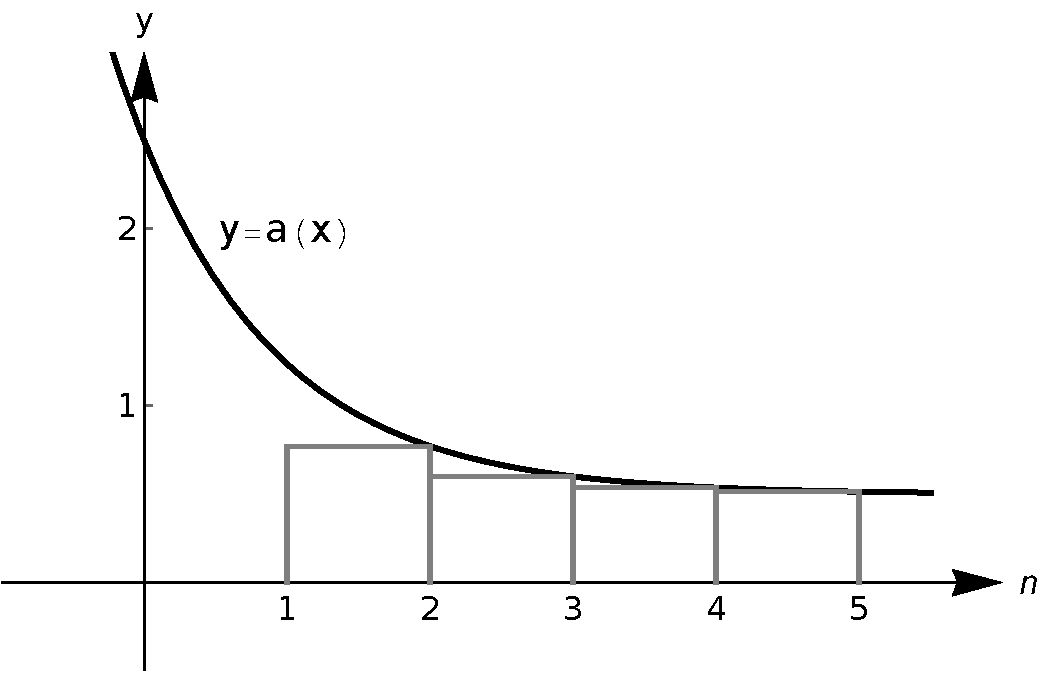
\includegraphics[width=0.5\textwidth]{fig_series_10b}
	\caption{Proving the integral test.}
	\label{fig_series_10a}
	\end{center}
\end{figure}

Consequently, it holds for the approximate area that
$$\ds \sum_{i=2}^n a_i<\ds\int\limits_1^n a(x)\ dx.$$
Now, let us suppose that
$$
\ds\int\limits_1^{+\infty} a(x)\ dx
$$
is convergent, so it must have a finite value. Also, because $a(x)$ is positive we know that
$$
\ds\int_1^n a(x)\ dx<\ds\int\limits_1^{+\infty} a(x)\ dx\,,
$$
from which we infer that
$$
\ds \sum_{i=2}^n a_i<\ds\int\limits_1^n a(x)\ dx<\ds\int\limits_1^{+\infty} a(x)\ dx.
$$
Our series of interest, however, starts at $n=1$, so we manipulate the last result to get
$$
\ds \sum_{i=1}^n a_i=a_1+\ds \sum_{i=2}^n a_i<a_1+\ds\int\limits_1^{+\infty} a(x)\ dx=M\,.
$$
This tells us that the sequence of partial sums $\ds \sum_{i=1}^n a_n$ is bounded above by $M$. Moreover, as the terms are positive we also know that,
$$
S_n\leq S_{n+1},
$$
i.e. the sequence $\left\{S_n\right\}_{n=1}^{+\infty}$ is also increasing and bounded above. Consequently, from Theorem~\ref{thm:monotonic_converge} this sequence of partial sums $\left\{S_n\right\}_{n=1}^{+\infty}$ is convergent, and hence is the considered series.
\end{proof}
%Bron: http://tutorial.math.lamar.edu/Classes/CalcII/IntegralTest.aspx#Series_IntTest_Proof


\fi

\ifcalculus
We can demonstrate the truth of this theorem with two simple graphs. In Figure \ref{fig_series_10a}, the height of each rectangle is $a(n)=a_n$ for $n=1,2,\ldots$, and clearly the rectangles enclose more area than the area under $y=a(x)$. Therefore we can conclude that \
\begin{equation}
\ds\int\limits_1^{+\infty} a(x)\ dx < \sum_{n=1}^{+\infty} a_n.
\label{eq:integral_testa}
\end{equation}


\begin{figure}
\centering
%\raisebox{0.5cm}{
\subfigure[\label{fig_series_10a}]{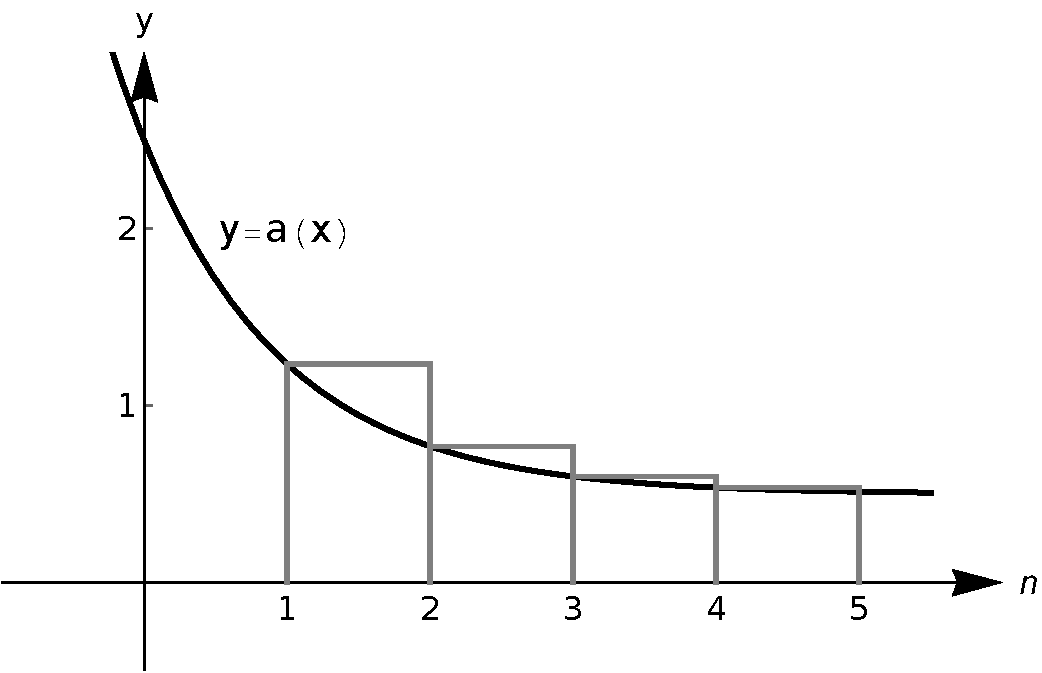
\includegraphics[width=0.45\textwidth]{fig_series_10a}}
\qquad
\subfigure[\label{fig_series_10b}]{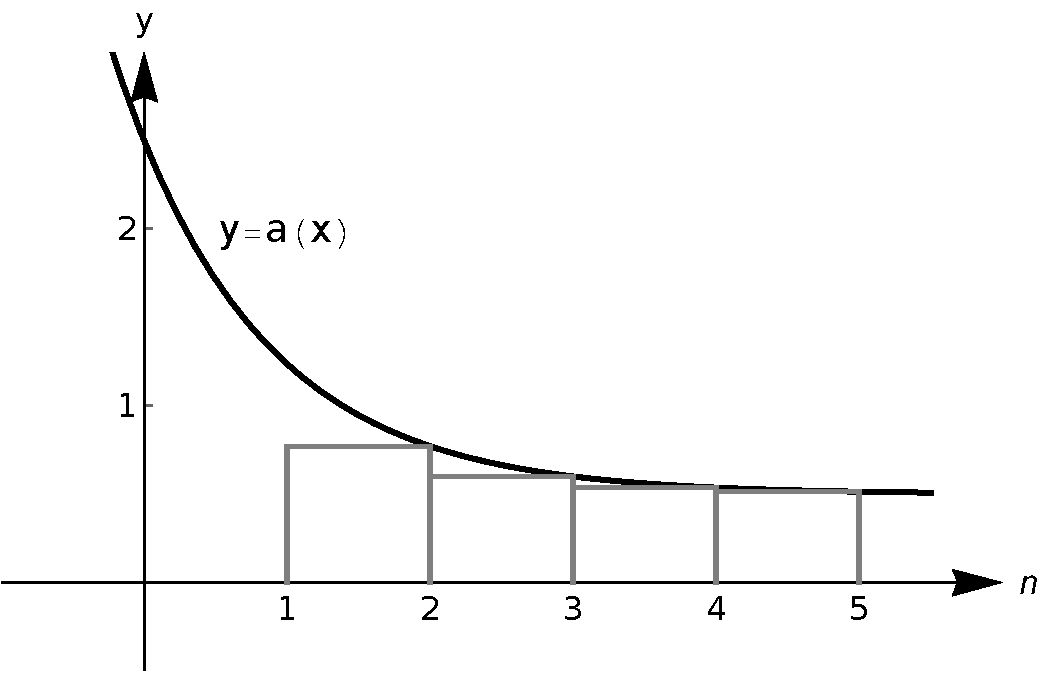
\includegraphics[width=0.45\textwidth]{fig_series_10b} }
\caption{Illustrating the truth of the integral test.}
\end{figure}


In Figure \ref{fig_series_10b}, we draw rectangles under $y=a(x)$ with the right-hand rule, starting with $n=2$. This time, the area of the rectangles is less than the area under $y=a(x)$, so
$$\ds\sum_{n=2}^{+\infty} a_n < \int\limits_1^{+\infty} a(x)\ dx.$$ Note how this summation starts with $n=2$; adding $a_1$ to both sides lets us rewrite the summation starting with $n=1$:
\begin{equation}\sum_{n=1}^{+\infty} a_n < a_1 +\int\limits_1^{+\infty} a(x)\ dx.\label{eq:integral_testb}
\end{equation} 

Combining Equations \eqref{eq:integral_testa} and \eqref{eq:integral_testb}, we have
\begin{equation}\sum_{n=1}^{+\infty} a_n< a_1 +\int\limits_1^{+\infty} a(x)\ dx < a_1 + \sum_{n=1}^{+\infty} a_n.\label{eq:integral_testc}\end{equation}
From Equation \eqref{eq:integral_testc} we can make the following two statements:
\begin{enumerate}
	\item If $\ds \sum_{n=1}^{+\infty} a_n$ diverges, so does $\ds\int\limits_1^{+\infty} a(x)\ dx$ because 
	$$\ds \sum_{n=1}^{+\infty} a_n < a_1 +\int\limits_1^{+\infty} a(x)\ dx.$$
	\item	If $\ds \sum_{n=1}^{+\infty} a_n$ converges, so does $\ds\int\limits_1^{+\infty} a(x)\ dx$ because 
	$$\ds \ds \int\limits_1^{+\infty} a(x)\ dx < \sum_{n=1}^{+\infty} a_n.$$
\end{enumerate}
\fi

\begin{example}\label{ex_itest1}
Determine the convergence of 
$$\ds\sum_{n=1}^{+\infty} \frac{\ln(n)}{n^2}.$$
The terms of the sequence $\{a_n\} = \{\ln(n)/n^2\}$ and the n$^{\text{th}}$ partial sums are given in Figure \ref{fig_series_11}.

\begin{figure}[H]
	\begin{center}
			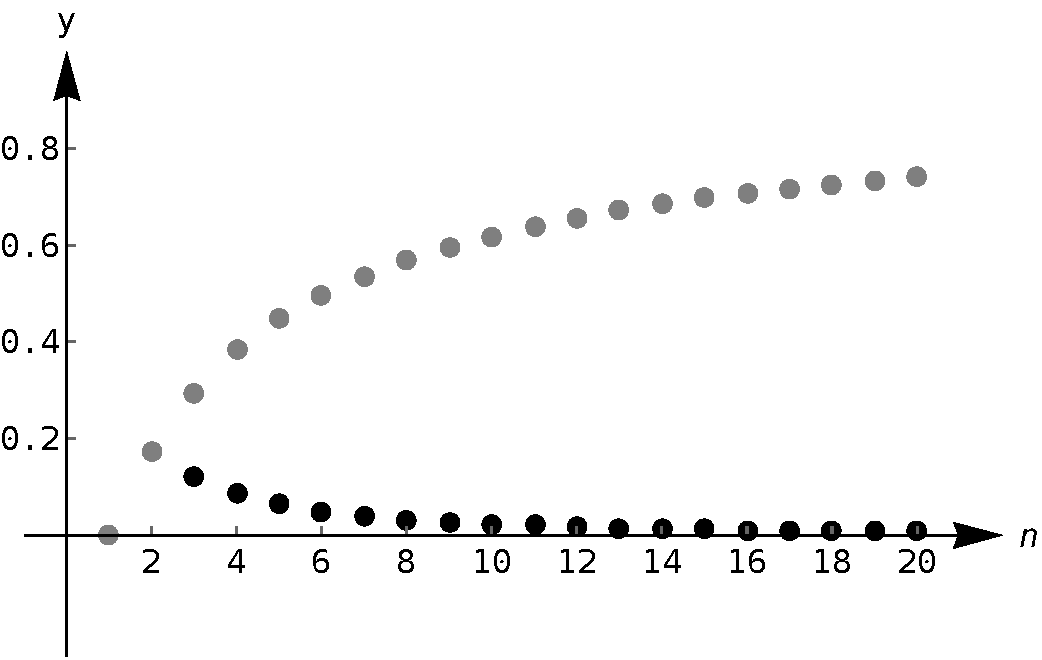
\includegraphics[width=0.5\textwidth]{fig_series_11}
	\caption{Plotting the terms (black) and partial series (gray) in Example \ref{ex_itest1}.}
	\label{fig_series_11}
	\end{center}
\end{figure}


\xhrulefill{gray}{2.5pt}Solution \xhrulefill{gray}{2.5pt}

Figure \ref{fig_series_11} implies that $a(n) = \ln(n)/n^2$ is positive and decreasing on $[2,+\infty\left[\right.$. We can determine this analytically, too. We know $a(n)$ is positive as both $\ln (n)$ and $n^2$ are positive on $[2,+\infty\left[\right.$. To determine that $a(n)$ is decreasing, consider the derivative of $a(n)$, i.e.\ $a'(n) = (1-2\ln(n))/n^3$, which is negative for $n\geq 2$. Since $a'(n)$ is negative, $a(n)$ is decreasing.


Applying the integral test, we test the convergence of $$\ds \int\limits_1^{+\infty} \frac{\ln(x)}{x^2}\ dx.$$ Integrating this improper integral requires the use of integration by parts, with $u = \ln(x)$ and $dv = 1/x^2\ dx$. 
\allowdisplaybreaks
\begin{align*}
\int\limits_1^{+\infty} \frac{\ln(x)}{x^2}\ dx &= \lim_{b\to+\infty} \int\limits_1^b \frac{\ln(x)}{x^2}\ dx\\[0.2cm]
				&= \lim_{b\to+\infty} \left[ -\frac1x\ln(x)\Bigg|_1^b + \int\limits_1^b\frac1{x^2}\ dx \right] \\[0.2cm]
%\end{align*}
%\begin{align*}
				&= \lim_{b\to+\infty} \left[-\frac1x\ln(x) -\frac 1x \right]\Bigg|_1^b\\[0.2cm]
				&= \lim_{b\to+\infty}\left[1-\frac1b-\frac{\ln(b)}{b}\right]\qquad \text{(Apply L'H\^opital's rule.)}\\
				&= 1.
\end{align*}
Since this improper integral converges, so does the studied series.
\end{example}

\ifanalysis

Theorem \ref{thm:pseries} was given without justification, stating that the general $p$-series 
$$\ds \sum_{n=1}^{+\infty} \frac 1{(an+b)^p}$$
converges if, and only if, $p>1$. Using the integral test, we can now prove this. 

\begin{proof}[of Theorem~\ref{thm:pseries}]
For that purpose, consider the following integral; assuming $p\neq 1$,
\begin{align*}
\int\limits_1^{+\infty} \frac1{(ax+b)^p}\ dx &= \lim_{c\to+\infty} \int\limits_1^c \frac1{(ax+b)^p}\ dx \\
		&= \lim_{c\to+\infty} \frac{1}{a(1-p)}(ax+b)^{1-p}\Big|_1^c\\
		&= \lim_{c\to+\infty} \frac{1}{a(1-p)}\big((ac+b)^{1-p}-(a+b)^{1-p}\big).
\end{align*}
This limit converges if, and only if, $p>1$. It is easy to show that the integral also diverges in the case of $p=1$. 

Therefore the general $p$-series converges if, and only if, $p>1$.
\end{proof}

\fi

\subsubsection{Limit comparison test}
We study one more convergence test, the so called limit comparison test. 

\begin{theorem}[Limit comparison test]\label{thm:series_limit_compare}
Let $\{a_n\}$ and $\{b_n\}$ be positive sequences. Then, the following holds.
\index{series!limit comparison test}\index{series!limit comparison test}\index{series!limit comparison test}
	\begin{enumerate}
		\item If $\ds\lim_{n\to+\infty} \frac{a_n}{b_n} = L$, where $L\in\mathbb{R}_0^+$, then $\ds \sum_{n=1}^{+\infty} a_n$ and $\ds \sum_{n=1}^{+\infty} b_n$ either both converge or both diverge.
		\item	If $\ds\lim_{n\to+\infty} \frac{a_n}{b_n} = 0$, then if $\ds \sum_{n=1}^{+\infty} b_n$ converges,  so does $\ds \sum_{n=1}^{+\infty} a_n$.
		\item	If $\ds\lim_{n\to+\infty} \frac{a_n}{b_n} = +\infty$, then if $\ds \sum_{n=1}^{+\infty} b_n$ diverges,  so does $\ds \sum_{n=1}^{+\infty} a_n$.
	\end{enumerate}
	\end{theorem}
	
	\checkoddpage
\marginpar{\ifoddpage\hspace*{-1.5cm}\else\hspace*{0.25cm}\fi
\includegraphics[width=0.075\textwidth]{youtube}\\
\ifoddpage\hspace*{-1.75cm}\else\hspace*{0.1cm}\fi
\qrcode[height=1.75cm]{https://youtu.be/AtbZZiSLemQ}
%\includegraphics[width=0.1\textwidth]{limit_comparison}
}

Theorem \ref{thm:series_limit_compare} is most useful when the convergence of the series from $\{b_n\}$ is known and we are trying to determine the convergence of the series from $\{a_n\}$. 

\ifanalysis

\begin{proof}
We prove the first statement of Theorem \ref{thm:series_limit_compare}.

Because $ \lim\limits _{n\to+\infty }{\frac {a_{n}}{b_{n}}}=L$  we know that for all $\varepsilon >0$ there is a positive integer $n_{0}$ such that for all $n\geq n_{0}$ we have that $\left|{\frac {a_{n}}{b_{n}}}-L\right|<\varepsilon$, or equivalently
$$
\displaystyle -\varepsilon <{\frac {a_{n}}{b_{n}}}-L<\varepsilon\,.
$$
From this, we infer that
$$
\displaystyle L-\varepsilon <{\frac {a_{n}}{b_{n}}}<L+\varepsilon \,,
$$
or
$$
\displaystyle (L-\varepsilon )b_{n}<a_{n}<(L+\varepsilon )b_{n}\,.
$$
As $L>0$ we can choose $\varepsilon$ to be sufficiently small such that $L-\varepsilon$  is positive. So $ b_{n}<{\frac {1}{L-\varepsilon }}a_{n}$ and by the direct comparison test, if $\ds \sum _{n}a_{n}$ converges then so does $\ds \sum _{n}b_{n}$. Similarly $a_{n}<(L+\varepsilon )b_{n}$, so if $\ds \sum _{n}b_{n}$ converges, again by the direct comparison test, so does $\ds \sum _{n}a_{n}$.

That is both series converge or both series diverge. 
\end{proof}

\fi

\begin{example}\label{ex_lct1}
Determine the convergence of
\begin{multicols}{2}
\begin{enumerate}
\item $\ds\sum_{n=1}^{+\infty} \frac1{n+\ln(n)}$
\item $\ds\sum_{n=1}^{+\infty} \frac{\sqrt{n}+3}{n^2-n+1}$
\end{enumerate}
\end{multicols}

\xhrulefill{gray}{2.5pt}Solution \xhrulefill{gray}{2.5pt}

\begin{enumerate}
\item We compare the terms of the studied series to the terms of the harmonic sequence:
\begin{align*}
\lim_{n\to+\infty}\frac{1/(n+\ln(n))}{1/n} &= \lim_{n\to+\infty} \frac{n}{n+\ln(n)} \\[0.2cm]
			&= 1\qquad \text{(after applying L'H\^opital's rule)}.
\end{align*}
Since the harmonic series diverges, we conclude that the investigated series diverges as well.
\item  We note that the dominant term in the expression of the series is $1/n^2$. Knowing that $\ds \sum_{n=1}^{+\infty} \frac1{n^2}$ converges, we attempt to apply the limit comparison test:
\begin{align*}
\lim_{n\to+\infty}\frac{(\sqrt{n}+3)/(n^2-n+1)}{1/n^2} &= \lim_{n\to+\infty}\frac{n^2(\sqrt n+3)}{n^2-n+1}\\[0.2cm]
		&= +\infty \qquad \text{(Apply L'H\^opital's rule)}.
\end{align*}

Theorem \ref{thm:series_limit_compare} part (3) only applies when $\ds\sum_{n=1}^{+\infty} b_n$ diverges; in our case, it converges. Ultimately, our test has not revealed anything about the convergence of our series.

The problem is that we chose a poor series with which to compare. Since the numerator and denominator of the terms of the series are both algebraic functions, we should have compared our series  to the dominant term of the numerator divided by the dominant term of the denominator. The dominant term of the numerator is $n^{1/2}$ and the dominant term of the denominator is $n^2$. Thus we should compare the terms of the given series to $n^{1/2}/n^2 = 1/n^{3/2}$:
\begin{align*}
\lim_{n\to+\infty}\frac{(\sqrt{n}+3)/(n^2-n+1)}{1/n^{3/2}} &= \lim_{n\to+\infty} \frac{n^{3/2}(\sqrt n+3)}{n^2-n+1} \\[0.2cm]
		&= 1\qquad \text{(Apply L'H\^opital's rule)}.
\end{align*}
Since the  $p$-series $\ds\sum_{n=1}^{+\infty} \frac1{n^{3/2}}$ converges, we conclude that the investigated series converges as well.
\end{enumerate}
\end{example}

The integral test does not work well with series containing factorial terms. The next section introduces the ratio test, which does handle such series well. We also introduce the root test, which is good for series where each term is raised to a power.

\subsection{Ratio and root tests}\label{sec:ratio_root_tests}


 This section introduces the ratio and root tests, which determine convergence by analysing the terms of a series to see if they approach 0 fast enough.

\subsubsection{Ratio test}

\begin{theorem}[Ratio test]\label{thm:ratio_test}
Let $\{a_n\}$ be a positive sequence where $\ds \lim_{n\to+\infty}\frac{a_{n+1}}{a_n} = L$.
\index{series!ratio comparison test}\index{convergence!ratio comparison test}\index{divergence!ratio comparison test}
		\begin{enumerate}
			\item If $L<1$, then $\ds\sum_{n=1}^{+\infty} a_n$ converges.
			\item	If $L>1$ or $L=+\infty$, then $\ds\sum_{n=1}^{+\infty} a_n$ diverges.
			\item If $L=1$, the ratio test is inconclusive.
		\end{enumerate}
\end{theorem}

Recall that Theorem \ref{thm:series_behavior} allows us to apply the ratio test to series where $\{a_n\}$ is positive for all but a finite number of terms. The principle of the ratio test is this: if  $L<1$, then for large $n$, each term of $\{a_n\}$ is significantly smaller than its previous term which is enough to ensure convergence.

\ifanalysis

\begin{proof}
Suppose first that 
$$\displaystyle L=\lim _{n\to+\infty }{\frac {a_{n+1}}{a_{n}}}<1.$$ Consider $r$ such that $L<r<1$ and it consequently for sufficiently large $n$ (say $N$) holds that 
$$
\dfrac{a_{n+1}}{a_n}\leq r\,.
$$
Equivalently, for $n\geq N$, we have that 
$$
a_{n+1}\leq r\,a_n\,.
$$
This implies that
$$ 
\begin{array}{rrcl}
&a_{N+1}&\leq&r\,a_N\\
\Leftrightarrow&a_{N+2}&\leq& r\,a_{N+1}\leq r^2\,a_N\\
\Leftrightarrow&a_{N+3}&\leq& r\,a_{N+2}\leq r^3\,a_N\\
&&\vdots&\\
\Leftrightarrow&a_{N+k}&\leq&r^k\,a_N
\end{array}
$$
for $k=0,1,2,\ldots$. Now, we can consider the sum of the terms in the left-hand sides of the above inequalities and hence compare 
$$
\sum\limits_{n=N}^{+\infty}a_n
$$
with the geometric series
$$
\sum\limits_{k=0}^{+\infty}r^k
$$
having $r<1$, it is clear that the former series must be convergent as the latter is and it constitutes an upper bound on the former. Finally, this leads us to conclude that the series under study
$$
\sum\limits_{n=1}^{+\infty}a_n=\sum\limits_{n=1}^{N-1}a_n+\sum\limits_{n=N}^{+\infty}a_n
$$
is convergent as well. 

Suppose now that 
$$\displaystyle L=\lim _{n\to+\infty }{\frac {a_{n+1}}{a_{n}}}>1.$$ Consider $r$ such that $1<r<L$ and it consequently for sufficiently large $n$ (say $N$) holds that 
$$
\dfrac{a_{n+1}}{a_n}\geq r\,.
$$
Is $N$ chosen such that $a_N>0$, then
$$
a_{N+k}\geq r^ka_N
$$
for $k=0,1,2,\ldots$. Since $r>1$, it is immediately clear that $\lim\limits_{n\to+\infty}a_n=+\infty$, from which we may conclude that the series under study is divergent. 

Suppose finally that $L=1$, then we can easily find an example that demonstrates the inconclusiveness of the ratio test for those cases. For instance, the harmonic series is known to be divergent, whereas a $p$-series with $p=2$ is convergent (Theorem~\ref{thm:pseries}).
\end{proof}

%Suppose that 
%$$\displaystyle L=\lim _{n\to+\infty }{\frac {a_{n+1}}{a_{n}}}<1.$$ We can then show that the series converges by showing that its terms will eventually become less than those of a certain convergent geometric series. 
%
%To do this, let $r={\frac {L+1}{2}}$. Then $r$ is strictly between $L$ and 1, and $\displaystyle a_{n+1}<ra_{n}$ for sufficiently large $n$ (say, $n$ greater than $N$). Hence $a_{n+i}<r^{i}a_{n}$ for each $n > N$ and $i > 0$, and so 
%$$
%{\displaystyle \sum _{i=N+1}^{+\infty }a_{i}=\sum _{i=1}^{+\infty }a_{N+i}<\sum _{i=1}^{+\infty }r^{i}a_{N+1}=a_{N+1}\sum _{i=1}^{+\infty }r^{i}=a_{N+1}{\frac {r}{1-r}}<+\infty .} $$
%That is, the series converges.
%
%On the other hand, if $L > 1$, then $\displaystyle a_{n+1}>a_{n}$ for sufficiently large n, so that the limit of the summands is non-zero because the terms are getting larger and guaranteed to not be negative. Hence the series diverges. 


\fi


\begin{example}\label{ex_ratio1}
Determine the convergence of the following series:
\begin{multicols}{3}
\begin{enumerate}
    \item $\ds 1.\ \sum_{n=1}^{+\infty} \frac{2^n}{n!}$
    \item $\ds\sum_{n=1}^{+\infty} \frac{3^n}{n^3} $
    \item $\ds\sum_{n=1}^{+\infty} \frac{1}{n^2+1}.$
    \end{enumerate}
\end{multicols}


\xhrulefill{gray}{2.5pt}Solution \xhrulefill{gray}{2.5pt}

\begin{enumerate}
	\item $\ds \sum_{n=1}^{+\infty} \frac{2^n}{n!}$
	\begin{align*}
	\lim_{n\to+\infty}\frac{2^{n+1}/(n+1)!}{2^n/n!} &= \lim_{n\to+\infty} \frac{2^{n+1}n!}{2^n(n+1)!}\\
				&= \lim_{n\to+\infty} \frac{2}{n+1}\\
				&=0.
	\end{align*}
	Since the limit is $0<1$, by the ratio test the considered series converges.
	
	\item	$\ds\sum_{n=1}^{+\infty} \frac{3^n}{n^3}$
	\begin{align*}
	\lim_{n\to+\infty} \frac{3^{n+1}/(n+1)^3}{3^n/n^3} &= \lim_{n\to+\infty}\frac{3^{n+1}n^3}{3^n(n+1)^3}\\
				&= \lim_{n\to+\infty} \frac{3n^3}{(n+1)^3}\\
				&= 3.
	\end{align*}
	Since the limit is $3>1$, by the ratio test the considered series diverges.
	
	\item  $\ds\sum_{n=1}^{+\infty} \frac{1}{n^2+1}$
	\begin{align*}
	\lim_{n\to+\infty} \frac{1/\big((n+1)^2+1\big)}{1/(n^2+1)} &= \lim_{n\to+\infty} \frac{n^2+1}{(n+1)^2+1}\\
				&= 1.
	\end{align*}
	Since the limit is 1, the ratio test is inconclusive. We can easily show this series converges using the direct or limit comparison tests, with each comparing to the series $$\ds \sum_{n=1}^{+\infty} \frac{1}{n^2}.$$
\end{enumerate}
\end{example}

The ratio test is not effective when the terms of a series only contain algebraic functions (e.g.\, polynomials). It is most effective when the terms contain some factorials or exponentials. The previous example also reinforces our developing intuition: factorials dominate exponentials, which dominate algebraic functions, which dominate logarithmic functions. In Part 1 of the example, the factorial in the denominator dominated the exponential in the numerator, causing the series to converge. In Part 2, the exponential in the numerator dominated the algebraic function in the denominator, causing the series to diverge.

\subsubsection{Root test}
The final test we introduce is the root test, which works particularly well on series where each term is raised to a power, and does not work well with terms containing factorials. %(but not those that include factorials). 

\begin{theorem}[Root test]\label{thm:root_test}
Let $\{a_n\}$ be a positive sequence, %such that there is an $N\geq 1$ where for all $n\geq N$, $a_n\geq 0$, 
and let $\ds \lim_{n\to+\infty} a_n^{1/n}= \lim_{n\to+\infty} \sqrt[n]{a_n} = L$.
\index{series!root comparison test}\index{convergence!root comparison test}\index{divergence!root comparison test}
		\begin{enumerate}
			\item If $L<1$, then $\ds\sum_{n=1}^{+\infty} a_n$ converges.
			\item	If $L>1$ or $L=+\infty$, then $\ds\sum_{n=1}^{+\infty} a_n$ diverges.
			\item If $L=1$, the root test is inconclusive.
		\end{enumerate}
\end{theorem}

\ifanalysis

\begin{proof}
This proof of the convergence is an application of the comparison test. If for all $n \geq N$ ($N$ some fixed natural number) we have $\displaystyle {\sqrt[{n}]{a_{n}}}\leq k<1$, then $a_{n}\leq k^{n}<1$. Since the geometric series $$\displaystyle \sum _{n=N}^{+\infty }k^{n}$$
converges so does 
$$\displaystyle \sum _{n=N}^{+\infty} a_{n}$$
by the comparison test.
\end{proof}


\fi

\begin{example}\label{ex_root1}
Determine the convergence of the following series:\\

\begin{multicols}{2}
\begin{enumerate}
    \item $\ds\sum_{n=1}^{+\infty} \left(\frac{3n+1}{5n-2}\right)^n$
    \item $\ds\sum_{n=1}^{+\infty} \frac{2^n}{n^2}.$
\end{enumerate}
\end{multicols}

\pagebreak
\xhrulefill{gray}{2.5pt}Solution \xhrulefill{gray}{2.5pt}

\begin{enumerate}
	\item We have that 
	$$\ds\lim_{n\to+\infty} \left(\left(\frac{3n+1}{5n-2}\right)^n\right)^{1/n} = \lim_{n\to+\infty} \frac{3n+1}{5n-2} = \frac 35.$$ 
	
	Since the limit is less than 1, we conclude the series converges. 
	
	
	\item	We see that
	$$\ds \lim_{n\to+\infty} \left(\frac{2^n}{n^2}\right)^{1/n} = \lim_{n\to+\infty} \frac{2}{\big(n^{1/n}\big)^2} = 2.$$ 
	
	Since this is greater than 1, we conclude the series diverges.
\end{enumerate}
\end{example}

 The next section considers alternating series, where the underlying sequence has terms that alternate between being positive and negative.


\section{Alternating series}\label{sec:alt_series}


All of the series convergence tests we have used require that the underlying sequence $\{a_n\}$ is a positive sequence. We can relax this with Theorem \ref{thm:series_behavior} and state that there must be an $N>0$ such that $a_n>0$ for all $n>N$; that is, $\{a_n\}$ is positive for all but a finite number of values of $n$. Here, we explore series whose summation includes negative terms. We start with a very specific form of series, where the terms of the summation alternate between being positive and negative.

\begin{definition}[Alternating series]\label{def:alt_series}
Let $\{a_n\}$ be a positive sequence. An \textbf{alternating series} (\textit{alternerende reeks}) is a series of either the form
\index{series!alternating}\index[aut]{reeks ! alternerend}
$$\sum_{n=1}^{+\infty} (-1)^na_n\qquad \text{or}\qquad \sum_{n=1}^{+\infty} (-1)^{n+1}a_n.$$
\end{definition}

Recall the terms of harmonic series come from the harmonic sequence $\{a_n\} = \{1/n\}$. An important alternating series is the alternating harmonic series:
$$\sum_{n=1}^{+\infty} (-1)^{n+1}\frac1n = 1-\frac12+\frac13-\frac14+\frac15-\frac16+\cdots\,.$$
\index{alternating harmonic series}\index[aut]{reeks ! alternerende harmonische}
\index{series ! alternating harmonic}

Geometric series can also be alternating series when $r<0$. For instance, if $r=-1/2$, the geometric series is
$$\sum_{n=0}^{+\infty} \left(\frac{-1}{2}\right)^n = 1-\frac12+\frac14-\frac18+\frac1{16}-\frac1{32}+\cdots\,.$$ 

Here, we have $r=-1/2$, so from Theorem \ref{thm:geom_series} we get
$$\sum_{n=0}^{+\infty} \left(\frac{-1}{2}\right)^n = \frac1{1-(-1/2)} = \frac 1{3/2} = \frac23.$$

A powerful convergence theorem exists for other alternating series that meet a few conditions.

\begin{theorem}[Alternating series test]\label{thm:alt_series_test}
Let $\{a_n\}$ be a monotonically decreasing, positive sequence with $a_n$ where $\ds \lim_{n\to+\infty}a_n=0$. Then
\index{series!Alternating Series Test}\index{alternating series test}\index{convergence!alternating series test}\index{divergence!alternating series test}
$$\sum_{n=1}^{+\infty} (-1)^{n}a_n \qquad \text{and}\qquad \sum_{n=1}^{+\infty} (-1)^{n+1}a_n$$ converge.
\end{theorem}

\ifanalysis

\begin{proof}
Suppose we are given a series of the form $\displaystyle \sum _{n=1}^{+\infty }(-1)^{n+1}a_{n}$, where $\displaystyle \lim _{n\rightarrow+\infty }a_{n}=0$ and $a_{n}\geq a_{n+1}$ for all natural numbers $n$. 

We will prove that both the partial sums 
$$
\displaystyle S_{2m+1}=\sum _{n=1}^{2m+1}(-1)^{n-1}a_{n}
$$
 with odd number of terms, and 
$$
\displaystyle S_{2m}=\sum _{n=1}^{2m}(-1)^{n-1}a_{n}
$$
 with even number of terms, converge to the same number $L$. Thus the usual partial sum 
$$
\displaystyle S_{k}=\sum _{n=1}^{k}(-1)^{n-1}a_{n}
$$
 also converges to $L$. 

We observe that the odd partial sums decrease monotonically:
$$
\displaystyle S_{2(m+1)+1}=S_{2m+1}-a_{2m+2}+a_{2m+3}\leq S_{2m+1}\,,
$$
 while the even partial sums increase monotonically:
$$
\displaystyle S_{2(m+1)}=S_{2m}+a_{2m+1}-a_{2m+2}\geq S_{2m}\,,
$$
because $a_{n}\geq a_{n+1}$.
Moreover, since $a_n$ are positive, $\displaystyle S_{2m+1}-S_{2m}=a_{2m+1}\geq 0$. Thus we can collect these facts to form the following inequality: 
$$
\displaystyle a_{1}-a_{2}=S_{2}\leq S_{2m}<S_{2m+1}\leq S_{1}=a_{1}.
$$
Now, note that $a_1 - a_2$ is a lower bound of the monotonically decreasing sequence $\left\{S_{2m+1}\right\}_{m=1}^{+\infty}$, the monotone convergence theorem (Theorem~\ref{thm:monotonic_converge}) then implies that this sequence converges as $m$ approaches infinity. Similarly, the sequence of even partial sum converges too. 

Finally, they must converge to the same number because
$$
\displaystyle \lim _{m\to+\infty }(S_{2m+1}-S_{2m})=\lim _{m\to+\infty }a_{2m+1}=0.
$$
This is illustrated in Figure~\ref{fig_series_12}. Since $\left\{S_{2m+1}\right\}_{m=1}^{+\infty}$ and $\left\{S_{2m}\right\}_{m=1}^{+\infty}$ converge, also $\left\{S_{m}\right\}_{m=1}^{+\infty}$ converges, and hence the studied alternating sequence also must converge. 
\end{proof}

\begin{figure}[h]
	\begin{center}
			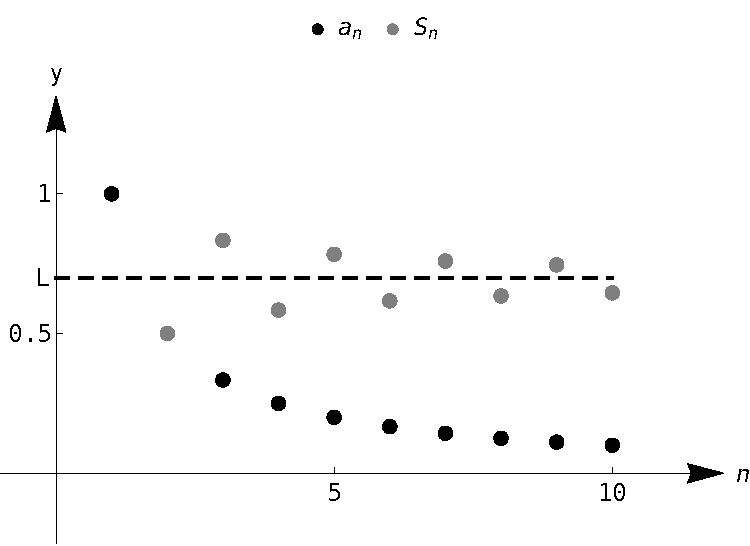
\includegraphics[width=0.5\textwidth]{fig_series_12}
	\caption{Illustrating convergence with the alternating series test.}
	\label{fig_series_12}
	\end{center}
\end{figure}




\fi

\ifcalculus
The basic idea behind Theorem \ref{thm:alt_series_test} is illustrated in Figure \ref{fig_series_12}. A positive, decreasing sequence $\{a_n\}$ is shown along with the partial sums
$$S_n = \sum_{i=1}^n(-1)^{i+1}a_i =a_1-a_2+a_3-a_4+\cdots+(-1)^{n+1}a_n.$$ 
Because $\{a_n\}$ is decreasing, the amount by which $S_n$ bounces up/down decreases. Moreover, the odd terms of $S_n$ form a decreasing, bounded sequence, while the even terms of $S_n$ form an increasing, bounded sequence. Since bounded, monotonic sequences converge (see Theorem \ref{thm:monotonic_converge}) and the terms of $\{a_n\}$ approach 0, one can show the odd and even terms of $S_n$ converge to the same common limit $L$, the sum of the series.


\begin{figure}
	\begin{center}
			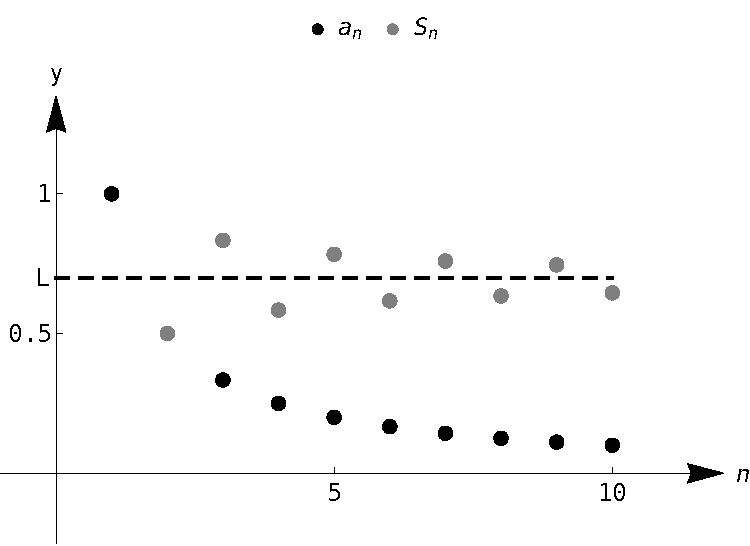
\includegraphics[width=0.5\textwidth]{fig_series_12}
	\caption{Illustrating convergence with the alternating series test.}
	\label{fig_series_12}
	\end{center}
\end{figure}


\fi

\begin{example}\label{ex_alt1}
Determine if the alternating series test applies to each of the following series.
\begin{multicols}{3}
\begin{enumerate}
    \item $\ds \sum_{n=1}^{+\infty} (-1)^{n+1}\frac1n$
    \item $\ds\sum_{n=1}^{+\infty} (-1)^n\frac{\ln(n)}{n}$ 
    \item $\ds\sum_{n=1}^{+\infty} (-1)^{n+1}\frac{|\sin(n)|}{n^2}$
\end{enumerate}
\end{multicols}


\xhrulefill{gray}{2.5pt}Solution \xhrulefill{gray}{2.5pt}

\begin{enumerate}
	\item This is the alternating harmonic series. The underlying sequence is $\{a_n\} = \{1/n\}$, which is positive, decreasing, and approaches 0 as $n\to+\infty$. Therefore we can apply the alternating series test and conclude this series converges. 
	
	
	\item		The underlying sequence is $\{a_n\} = \{\ln(n)/n\}$. This is positive and approaches 0 as $n\to+\infty$ (use L'H\^opital's rule). However, the sequence is not decreasing for all $n$. It is straightforward to compute $a_1=0$, $a_2\approx0.347$, $a_3\approx 0.366$, and $a_4\approx 0.347$: the sequence is increasing for at least the first 3 terms. 
	
	We do not immediately conclude that we cannot apply the alternating series test. Rather, consider the long--term behaviour of $\{a_n\}$. Treating $a_n=a(n)$ as a continuous function of $n$ defined on $[1,+\infty\left[\right.$, we can take its derivative:
	$$a'(n) = \frac{1-\ln(n)}{n^2}.$$
	The derivative is negative for all $n\geq 3$ (actually, for all $n\geq e$), meaning $a(n)=a_n$ is decreasing on $[3,+\infty[$. We can apply the alternating series test to the series when we start with $n=3$ and conclude that the investigated series converges; adding the terms with $n=1$ and $n=2$ do not change the convergence (i.e., we apply Theorem \ref{thm:series_behavior}). The important lesson here is that as before, if a series fails to meet the criteria of the alternating series test on only a finite number of terms, we can still apply the test.
	
	\item  The underlying sequence is $\{a_n\} = |\sin(n)|/n^2$. This sequence is positive and approaches $0$ as $n\to+\infty$. However, it is not a decreasing sequence; the value of $|\sin(n)|$ oscillates between $0$ and $1$ as $n\to+\infty$. We cannot remove a finite number of terms to make $\{a_n\}$ decreasing, therefore we cannot apply the alternating series test. Keep in mind that this does not mean we conclude the series diverges; in fact, it does converge. We are just unable to conclude this based on Theorem \ref{thm:alt_series_test}.
\end{enumerate}
\end{example}


While there are many factors involved when studying rates of convergence, the alternating structure of an alternating series gives us a powerful tool when approximating the sum of a convergent series. 

\begin{theorem}[The alternating series approximation theorem]\label{thm:alt_series_approx}
Let $\{a_n\}$ be a sequence that satisfies the hypotheses of the alternating series test, and let $S_n$ and $L$ be the $n^\text{th}$ partial sums and sum, respectively, of either $\ds \sum_{n=1}^{+\infty} (-1)^{n}a_n$ or $\ds \sum_{n=1}^{+\infty} (-1)^{n+1}a_n$. Then
\begin{enumerate}
	\item $|S_n-L| < a_{n+1}$, and
	\item	$L$ is between $S_n$ and $S_{n+1}$.
\end{enumerate}
\end{theorem}

\ifanalysis

\begin{proof}
Essentially, the limit of the converging sequences $\left\{S_{2m+1}\right\}_{m=1}^{+\infty}$ and $\left\{S_{2m}\right\}_{m=1}^{+\infty}$  in the proof of Theorem~\ref{thm:alt_series_test} is the sum $L$. So, the monotone convergence theorem also tells us that
\begin{equation}
\displaystyle S_{2m}\leq L\leq S_{2m+1}
\label{alteq}
\end{equation}
for any $m$. This means the partial sums of an alternating series also alternates above and below the final limit. More precisely, when there are odd (even) number of terms, i.e. the last term is a plus (minus) term, then the partial sum is above (below) the final limit. 

Now, we would like to show $\displaystyle \left|S_{n}-L\right|\leq a_{n+1}$ by splitting into two cases.

When $n = 2m+1$, i.e. odd, then 
$$
\displaystyle \left|S_{2m+1}-L\right|=S_{2m+1}-L\leq S_{2m+1}-S_{2m+2}=a_{(2m+1)+1}
$$

When $n = 2m$, i.e. even, then
$$
\displaystyle \left|S_{2m}-L\right|=L-S_{2m}\leq S_{2m+1}-S_{2m}=a_{2m+1}
$$
as desired. Both statements from Inequality~\eqref{alteq}. 
\end{proof}

\fi

Part 1 of Theorem \ref{thm:alt_series_approx} states that the $n^\text{th}$ partial sum of a convergent alternating series will be within $a_{n+1}$ of its total sum. Consider the alternating series 
$$\ds \sum_{n=1}^{+\infty} \frac{(-1)^{n+1}}{n^2}.$$
 Since $a_{14} = 1/14^2 \approx 0.0051$, we know that $S_{13}$ is within $0.0051$ of the total sum. %That is, we know $S_{13}$ is accurate to at least 1 place after the decimal. (The ``5'' in the third place after the decimal could cause a carry meaning $S_{13}$ isn't accurate to two places after the decimal; in this particular case, that doesn't happen.) 

Moreover, Part 2 of the theorem states that since $S_{13} \approx 0.8252$ and $S_{14}\approx 0.8201$, we know the sum $L$ lies between $0.8201$ and $0.8252$. One use of this is the knowledge that $S_{14}$ is accurate to two places after the decimal.

Some alternating series converge slowly. In Example \ref{ex_alt1} we determined that  series $$\ds\sum_{n=1}^{+\infty} (-1)^{n+1}\frac{\ln(n)}{n}$$ converged. With $n=1001$, we find $\ln(n)/n \approx 0.0069$, meaning that $S_{1000} \approx 0.1633$ is accurate to one, maybe two, places after the decimal. Since $S_{1001} \approx 0.1564$, we know the sum $L$ is $0.1564\leq L\leq0.1633$.


Sometimes, the signs of the terms in a series can have a significant impact on the convergence of a series. This leads us to the following definitions. 

\begin{definition}[Absolute and conditional convergence] \label{def:abs_converge}
{\footnotesize $\,$}\\
\vspace*{-1.25cm}
\begin{enumerate}
	\item  A series $\ds \sum_{n=1}^{+\infty} a_n$ converges \textbf{absolutely} (\textit{absoluut}) if $\ds \sum_{n=1}^{+\infty} |a_n|$ converges.
	\index{convergence!absolute}\index{convergence!conditional}\index{series!absolute convergence}\index{series!conditional convergence}
	\item A series $\ds \sum_{n=1}^{+\infty} a_n$ converges \textbf{conditionally} (\textit{voorwaardelijk}) if $\ds \sum_{n=1}^{+\infty} a_n$ converges but $\ds \sum_{n=1}^{+\infty} |a_n|$ diverges.\index[aut]{reeks ! absolute convergentie}\index[aut]{reeks ! voorwaardelijke convergentie}
\end{enumerate}
\end{definition}

\begin{example}\label{ex_alt_series2}
Determine if the following series converge absolutely, conditionally, or diverge.
\begin{multicols}{2}
\begin{enumerate}
    \item  $\ds  \sum_{n=1}^{+\infty} (-1)^n\frac{n+3}{n^2+2n+5}$
    \item $\ds \sum_{n=1}^{+\infty} (-1)^n\frac{n^2+2n+5}{2^n}$
\end{enumerate}
\end{multicols}


\xhrulefill{gray}{2.5pt}Solution \xhrulefill{gray}{2.5pt}

\begin{enumerate}
	\item We can show the series $$\ds \sum_{n=1}^{+\infty} \left|(-1)^n\frac{n+3}{n^2+2n+5}\right|= \sum_{n=1}^{+\infty} \frac{n+3}{n^2+2n+5}$$ diverges using the limit comparison test, comparing with $1/n$. 
	
	The investigated series  converges using the alternating series test; we conclude it converges conditionally.
	
	\item	We can show the series $$\ds \sum_{n=1}^{+\infty} \left|(-1)^n\frac{n^2+2n+5}{2^n}\right|=\sum_{n=1}^{+\infty} \frac{n^2+2n+5}{2^n}$$  converges using the ratio test. 
	
	Therefore we conclude that the studied series converges absolutely.
	
\end{enumerate}
\end{example}

Knowing that a series converges absolutely allows us to make two important statements, given in the following theorem.


	\checkoddpage
\marginpar{\ifoddpage\hspace*{-1.5cm}\else\hspace*{0.25cm}\fi
\includegraphics[width=0.075\textwidth]{youtube}\\
\ifoddpage\hspace*{-1.75cm}\else\hspace*{0.1cm}\fi
\qrcode[height=1.75cm]{https://youtu.be/ORTI4kk1okM}
%\includegraphics[width=0.1\textwidth]{abs_conv}
}


\begin{theorem}[Absolute convergence theorem]\label{thm:abs_convergence}
{\footnotesize $\,$}\vspace*{-0.75cm}

Let $\ds \sum_{n=1}^{+\infty} a_n$ be a series that converges absolutely.
\index{convergence!absolute}\index{absolute convergence theorem}\index{series!absolute convergence theorem}\index{rearrangements of series}\index{series!rearrangements}
\begin{enumerate}
	\item $\ds \sum_{n=1}^{+\infty} a_n$ converges.
	
	\item	Let $\{b_n\}$ be any rearrangement of the sequence $\{a_n\}$. Then 
	$$ \sum_{n=1}^{+\infty} b_n = \sum_{n=1}^{+\infty} a_n.$$
\end{enumerate}
\end{theorem}

\ifanalysis

\begin{proof}
To prove the first statement of this theorem, first notice that $\left|a_n\right|$ is either $a_n$ or it is $-a_n$ depending on its sign.  This means that we can then say,
$$
0\leq a_n+\left|a_n\right|\leq 2\left|a_n\right|\,.
$$
Now, since we are assuming that $\ds \sum_{n=1}^{+\infty} \left|a_n\right|$ is convergent also $\ds \sum_{n=1}^{+\infty} 2\left|a_n\right|$ is convergent since we can just factor the 2 out of the series and 2 times a finite value will still be finite.  This however allows us to use the comparison test to say that
$$
\ds \sum_{n=1}^{+\infty} \left(a_n+\left|a_n\right| \right)
$$
is also a convergent series. Finally, we can write
$$
\ds \sum_{n=1}^{+\infty} a_n=\ds \sum_{n=1}^{+\infty} \left(a_n+\left|a_n\right|\right)-\ds \sum_{n=1}^{+\infty} \left|a_n\right|\,,
$$
so $\ds \sum_{n=1}^{+\infty} a_n$ is the difference of two convergent series and hence is also convergent.
\end{proof}

\fi

The first statement of Theorem~\ref{thm:abs_convergence} tells us  that absolute convergence is  stronger than regular convergence. That is, just because {\small$\ds \sum_{n=1}^{+\infty} a_n$} converges, we cannot conclude that {\small$\ds \sum_{n=1}^{+\infty} |a_n|$} will converge, but knowing a series converges absolutely tells us that {\small$\ds \sum_{n=1}^{+\infty} a_n$} will converge. For instance, in Example \ref{ex_alt_series2}, we determined the series in Part 2 converges absolutely. Theorem \ref{thm:abs_convergence} tells us the series converges

One reason this is important is that our convergence tests all require that the underlying sequence of terms be positive. By taking the absolute value of the terms of a series where not all terms are positive, we are often able to apply an appropriate test and determine absolute convergence. This, in turn, determines that the series we are given also converges.

The second statement relates to \textbf{rearrangements}\index{rearrangements of series}\index{series!rearrangements} of series. When dealing with a finite set of numbers, the sum of the numbers does not depend on the order which they are added. (So $1+2+3 = 3+1+2$.) One may be surprised to find out that when dealing with an infinite set of numbers, the same statement does not always hold true: some infinite lists of numbers may be rearranged in different orders to achieve different sums. The theorem states that the terms of an absolutely convergent series can be rearranged in any way without affecting the sum.

This implies that perhaps the sum of a conditionally convergent series can change based on the arrangement of terms. Indeed, it can. The so-called Riemann rearrangement theorem  states that any conditionally convergent series can have its terms rearranged so that the sum is any desired value, including $+\infty$.

As an example, consider the alternating harmonic series once more. We have stated that 
$$\sum_{n=1}^{+\infty} (-1)^{n+1}\frac1n = 1-\frac12+\frac13-\frac14+\frac15-\frac16+\frac17\cdots = \ln (2).$$

Consider the rearrangement where every positive term is followed by two negative terms:
$$
1-\frac12-\frac14+\frac13-\frac16-\frac18+\frac15-\frac1{10}-\frac1{12}\cdots .
$$
Now group some terms and simplify:
\begin{align*}
\left(1-\frac12\right)-\frac14+\left(\frac13-\frac16\right)-\frac18+\left(\frac15-\frac1{10}\right)-\frac1{12}+\cdots & \\
=\frac12-\frac14+\frac16-\frac18+\frac1{10}-\frac{1}{12}+\cdots & \\
=\frac12\left(1-\frac12+\frac13-\frac14+\frac15-\frac16+\cdots\right) & = \frac12\ln (2).
\end{align*}

By rearranging the terms of the series, we have arrived at a different sum! \ifanalysis One could try to argue that the Alternating Harmonic Series does not actually converge to $\ln (2)$, because rearranging the terms of the series should not change the sum. However, the Alternating Series Test proves this series converges to $L$, for some number $L$, and if the rearrangement does not change the sum, then $L = L/2$, implying $L=0$. But the alternating series approximation theorem quickly shows that $L>0$. The only conclusion is that the rearrangement did change the sum. \fi This is an incredible result.

While series are worthy of study in and of themselves, our ultimate goal within calculus is the study of power series, which we will consider in the next section. We will use power series to create functions where the output is the result of an infinite summation.

\section{Power series}\label{sec:power_series}

So far, our study of series has examined the question of ``Is the sum of these infinite terms finite?,'' i.e., ``Does the series converge?'' We now approach series from a different perspective: as a function. Given a value of $x$, we evaluate $f(x)$ by finding the sum of a particular series that depends on $x$ (assuming the series converges). We start this new approach to series with a definition.

\pagebreak

\begin{definition}[Power series]\label{def:power_series}
Let $\{a_n\}$ be a sequence, let $x$ be a variable, and let $x_0$ be a real number.
\index{power series}\index{series!power}\index[aut]{machtreeks}
	\begin{enumerate}
		\item The \textbf{power series} (\textit{machtreeks}) in $x$ is the series
		$$\sum_{n=0}^{+\infty} a_nx^n = a_0+a_1x+a_2x^2+a_3x^3+\ldots$$
		
		\item The power series in $x$ centred at $x_0$ is the series
		$$\sum_{n=0}^{+\infty} a_n(x-x_0)^n = a_0+a_1(x-x_0)+a_2(x-x_0)^2+a_3(x-x_0)^3+\ldots$$
	\end{enumerate}
\end{definition}

For instance, 
$$
\sum_{n=1}^{+\infty} (-1)^{n+1}\frac{(x+1)^n}{n}
$$
is a power series centred at $x_0=-1$.  Note how this series starts with $n=1$. We could, however, rewrite it starting at $n=0$ with the understanding that $a_0=0$, and hence the first term is $0$. Anyhow, its first five terms are given by:
	$$\sum_{n=1}^{+\infty} (-1)^{n+1}\frac{(x+1)^n}n = (x+1) - \frac{(x+1)^2}{2} + \frac{(x+1)^3}{3} - \frac{(x+1)^4}{4}+\frac{(x+1)^5}{5}\ldots$$
	
Of course, not every series converges. This makes us wonder for what values of $x$ will a given power series converge? Which  leads us to a theorem and definition.


\begin{theorem}[Convergence of power series]\label{thm:radius_converge}
{\footnotesize $\,$}\\
\vspace*{-1.25cm}

Let a power series $\ds \sum_{n=0}^{+\infty} a_n(x-x_0)^n$ be given. Then one of the following is true:
\index{power series!convergence}\index[aut]{machtreeks ! convergentie}
\begin{enumerate}
	\item The series converges only at $x=x_0$.
	\item	There is an $R>0$ such that the series converges for all $x$ in $\left.\right]x_0-R,x_0+R\left[\right.$ and diverges for all $x<x_0-R$ and $x>x_0+R$.
	\item	The series converges for all $x$.
\end{enumerate}
\end{theorem}

Note that part 2 of this theorem  makes a statement about the interval $\left.\right]x_0-R,x_0+R\left[\right.$, but not the endpoints of that interval. A series may/may not converge at these endpoints. The value of $R$ is important when understanding a power series, hence it is given a name in the following definition.


\begin{definition}[Radius and interval of convergence]\label{def:radius_converge}
 \begin{enumerate}
		\item The number $R$ given in Theorem \ref{thm:radius_converge} is the \textbf{radius of convergence} (\textit{convergentiestraal}) of a given series. When a series converges for only $x=x_0$, we say the radius of convergence is 0, i.e.,  $R=0$. When a series converges for all $x$, we say the series has an infinite radius of convergence, i.e., $R=+\infty$.
			\item	The \textbf{interval of convergence} (\textit{convergentie-interval}) is the set of all values of $x$ for which the series converges.
			\index{convergence!radius of}\index{convergence!interval of}\index{radius of convergence}\index{interval of convergence}\index{series!radius of convergence}\index{series!interval of convergence}\index[aut]{machtreeks ! convergentiestraal}\index[aut]{machtreeks ! convergentiegebied}
	\end{enumerate}
\end{definition}

\ifanalysis

The radius of convergence can be found using the following theorem.

\begin{theorem}[Cauchy-Hadamard theorem]\label{thm:cauchy}
The radius of convergence $R$ of the power series
$$\ds \sum_{n=0}^{+\infty} a_n(x-x_0)^n$$
is given by
$$
\displaystyle R={\frac {1}{\ds \limsup _{n\rightarrow +\infty }{\sqrt[{n}]{|a_{n}|}}}}\,,
$$
where $R= 0$ if the lim sup diverges to $+\infty$, and $R=+\infty$ if the lim sup is 0.
\end{theorem}

	\checkoddpage
\marginpar{\ifoddpage\hspace*{-1.5cm}\else\hspace*{0.25cm}\fi
\includegraphics[width=0.075\textwidth]{youtube}\\
\ifoddpage\hspace*{-1.75cm}\else\hspace*{0.1cm}\fi
\qrcode[height=1.75cm]{https://youtu.be/ADVZOhMDmQI}
%\includegraphics[width=0.1\textwidth]{figures/Series/limsup.png}
}

\begin{proof}
This theorem can be proved by considering the number used in the root test:
$$
\displaystyle C=\limsup _{n\rightarrow +\infty }{\sqrt[{n}]{|a_{n}(x-x_0)^{n}|}}=\limsup _{n\rightarrow +\infty }{\sqrt[{n}]{|a_{n}|}}|x-x_0|.
$$
The root test states that the series converges if $C < 1$ and diverges if $C > 1$. It follows immediately that the power series converges if the distance from $x$ to the centre $x_0$ is less than
$$
\displaystyle R={\frac {1}{\ds \limsup _{n\rightarrow +\infty }{\sqrt[{n}]{|a_{n}|}}}}
$$
and diverges if the distance exceeds that number.
\end{proof}

\fi

In practice, however, to find the values of $x$ for which a given series converges, we will use the convergence tests we studied previously. However, the tests all required that the terms of a series be positive. The following theorem gives us a work--around to this problem.

\begin{theorem}[The radius of convergence of a series and absolute convergence]\label{thm:abs_power}
{\footnotesize $\,$}\vspace*{-0.75cm}

	The series $\ds \sum_{n=0}^{+\infty} a_n(x-x_0)^n$ and $\ds \sum_{n=0}^{+\infty} \big|a_n(x-x_0)^n\big|$ have the same radius of convergence $R$.
%\end{itemize}
\end{theorem}
\ifanalysis

\begin{proof}
This theorem is an immediate consequence of the proof of the Cauchy-Hadamard theorem. 
\end{proof}

\fi

Theorem \ref{thm:abs_power} allows us to find the radius of convergence $R$ of a series by applying the ratio test (or any applicable test) to the absolute value of the terms of the series. We practice this in the following example.


\begin{example}\label{ex_ps2}
Find the radius and interval of convergence for each of the following series:
\begin{multicols}{3}
\begin{enumerate}
\item $\ds \sum_{n=1}^{+\infty} (-1)^{n+1}\frac{x^n}{n}$
\item $\ds \sum_{n=0}^{+\infty} 2^n(x-3)^n$
\item $\ds \sum_{n=0}^{+\infty} n!x^n$
\end{enumerate}
\end{multicols}

\pagebreak
\xhrulefill{gray}{2.5pt}Solution \xhrulefill{gray}{2.5pt}

\begin{enumerate}
		
	\item		We apply the ratio test to the series $$\ds \sum_{n=1}^{+\infty} \left|(-1)^{n+1}\frac{x^n}{n}\right| = \sum_{n=1}^{+\infty} \left|\frac{x^n}{n}\right|.$$ We have
	\begin{align*}
	\lim_{n\to+\infty} \frac{\big|x^{n+1}/(n+1)\big|}{\big|x^n/n\big|} &= \lim_{n\to+\infty} \left|\frac{x^{n+1}}{x^n}\cdot \frac{n}{n+1}\right| \\
			&= \lim_{n\to+\infty} |x|\frac{n}{n+1}\\
			&= |x|.
	\end{align*}
	The ratio test states a series converges if the limit of $|a_{n+1}/a_n| = L<1$. We found the limit above to be $|x|$; therefore, the studied power series converges when $|x| <1$, or when $x$ is in $\left.\right]-1,1\left[\right.$. Thus the radius of convergence is $R=1$.

	
	To determine the interval of convergence, we need to check the endpoints of $\left.\right]-1,1\left[\right.$. When $x=-1$, we have the opposite of the harmonic series:
	$$
	\sum_{n=1}^{+\infty} (-1)^{n+1}\frac{(-1)^n}{n} = \sum_{n=1}^{+\infty} \frac{-1}{n}= -\infty.$$

	This series diverges when $x=-1$.
	
	When $x=1$, we have the series $$\ds \sum_{n=1}^{+\infty} (-1)^{n+1}\frac{(1)^n}{n},$$
	which is the alternating harmonic series, which converges conditionally. Therefore the interval of convergence is $\left.\right]-1,1]$.
	
	\item		We apply the ratio test to the series $$\ds\sum_{n=0}^{+\infty} \big|2^n(x-3)^n\big|.$$
	We have
	\begin{align*}
	\lim_{n\to+\infty} \frac{\big| 2^{n+1}(x-3)^{n+1}\big|}{\big|2^n(x-3)^n\big|} &= \lim_{n\to+\infty} \left|\frac{2^{n+1}}{2^n}\cdot\frac{(x-3)^{n+1}}{(x-3)^n}\right|\\
			&=\lim_{n\to+\infty} \big|2(x-3)\big|.
	\end{align*}
	
According to the ratio test, the series converges when $\big|2(x-3)\big|<1$ so when $\big|x-3\big| < 1/2$. The series is centred at 3, and $x$ must be within $1/2$ of 3 in order for the series to converge. Therefore the radius of convergence is $R=1/2$, and we know that the series converges absolutely for all $x$ in $\left.\right]3-1/2,3+1/2\left[\right. = \left.\right]2.5, 3.5\left[\right.$.

We check for convergence at the endpoints to find the interval of convergence. When $x=2.5$, we have:
\begin{align*}
\sum_{n=0}^{+\infty} 2^n(2.5-3)^n &= \sum_{n=0}^{+\infty} 2^n\left(-\dfrac{1}{2}\right)^n \\
			&=\sum_{n=0}^{+\infty} (-1)^n,
\end{align*}
which diverges. A similar process shows that the series also diverges at $x=3.5$. Therefore the interval of convergence is $\left.\right]2.5, 3.5\left[\right.$.

\item	We apply the ratio test to $\ds \sum_{n=0}^{+\infty} \big|n!x^n\big|$. \\
We have
\begin{align*}
\lim_{n\to+\infty} \frac{\big| (n+1)!x^{n+1}\big|}{\big|n!x^n\big|} &= \lim_{n\to+\infty} \big|(n+1)x\big|\\
		&= +\infty
\end{align*}
for all $x$, except $x=0$.


The ratio test shows that the series diverges for all $x$ except $x=0$. Therefore the radius of convergence is $R=0$.
\end{enumerate}
\end{example}


We can use a power series to define a function:
$$f(x) = \sum_{n=0}^{+\infty} a_nx^n,$$
where the domain of $f$ is a subset of the interval of convergence of the power series. One can apply calculus techniques to such functions; in particular, we can find derivatives and antiderivatives. 


	\checkoddpage
\marginpar{\ifoddpage\hspace*{-1.5cm}\else\hspace*{0.25cm}\fi
\includegraphics[width=0.075\textwidth]{youtube}\\
\ifoddpage\hspace*{-1.75cm}\else\hspace*{0.1cm}\fi
\qrcode[height=1.75cm]{https://youtu.be/5ygANwfTCHc}
%\includegraphics[width=0.1\textwidth]{reeksen_afleiden}
}

\begin{theorem}[Derivatives and indefinite integrals of power series]\label{thm:calc_power_series}
{\footnotesize $\,$}\vspace*{-0.75cm}

Let $\ds f(x) = \sum_{n=0}^{+\infty} a_n(x-x_0)^n$ be a function defined by a power series, with radius of convergence $R$. Then the following hold: 
	\begin{enumerate}
		\item $f(x)$ is continuous and differentiable on $[x_0-R,x_0+R]$.
		\item	$\ds \fp(x) = \sum_{n=1}^{+\infty} a_n\cdot n\cdot (x-x_0)^{n-1}$, with radius of convergence $R$.
		\item	$\ds \int f(x)\ dx = x_0+\sum_{n=0}^{+\infty} a_n\frac{(x-x_0)^{n+1}}{n+1}$, with radius of convergence $R$.
		\index{integration!power series}\index{derivative!power series}\index{power series!derivatives and integrals}
		\index[aut]{machtreeks ! afleiden}
		\index[aut]{machtreeks ! integreren}
	\end{enumerate}
\end{theorem}

Note that this theorem states that differentiation and integration do not change the radius of convergence. It does not state anything about the interval of convergence. They are not always the same. Moreover, differentiation and integration are simply calculated term--by--term using the power rules.

\ifanalysis

\begin{proof}
We omit the proof of this theorem due to its technicality, but still its statements are relatively easy to understand by applying differentiation and integration termwise. 
\end{proof}

\fi

We can learn a great deal from taking derivatives and indefinite integrals of power series functions.  For instance, consider 
$$\ds f(x) = \sum_{n=0}^{+\infty} x^n,$$
which is a geometric series. According to Theorem \ref{thm:geom_series}, this series converges to $1/(1-x)$ when $|x|<1$. Thus we can say
$$	f(x) = \sum_{n=0}^{+\infty} x^n = \frac 1{1-x},\quad \text{ on }\quad \left.\right]-1,1\left[\right..$$

Integrating the power series, we find
\begin{equation} F(x)  = C_1+\sum_{n=0}^{+\infty} \frac{x^{n+1}}{n+1},\label{eq:ps3a}\end{equation}
while integrating the function $f(x) = 1/(1-x)$ gives
\begin{equation} F(x)  = -\ln|1-x| + C_2.\label{eq:ps3b}\end{equation}

Equating Equations \eqref{eq:ps3a} and \eqref{eq:ps3b}, we have 
$$F(x) = C_1+\sum_{n=0}^{+\infty} \frac{x^{n+1}}{n+1} = -\ln|1-x| + C_2.$$
Letting $x=0$, we have $F(0) = C_1 = C_2$. This implies that we can drop the constants and conclude
\begin{equation}
\sum_{n=0}^{+\infty} \frac{x^{n+1}}{n+1} = -\ln|1-x|.
\label{eq:ps3c}\end{equation}
At $x=-1$, we have
$$F(-1) = -1+\frac12-\frac13+\frac14-\frac15+\cdots$$
Notice that this series is an alternating series whose terms converge to 0. By the alternating series test, this series converges. In fact, we can recognize that its terms are the opposite of the alternating harmonic series. We can thus say that $F(-1) = -\ln(2)$.

Since,  the series on the left of Equation~\eqref{eq:ps3c} converges at $x=-1$; substituting $x=-1$ on both sides of the above equality gives
$$-1+\frac12-\frac13+\frac14-\frac15+\cdots = -\ln(2).$$
 We conclude that 
$$1-\frac12+\frac13-\frac14+\cdots = \ln(2).$$
This shows that the alternating harmonic series converges to $\ln (2)$. \index{alternating harmonic series}\index[aut]{alternerende harmonische reeks}


\begin{example}\label{ex_ps4}
{\footnotesize $\,$\\}
Let $\ds f(x) = \sum_{n=0}^{+\infty} \frac{x^n}{n!}$. Find $\ds \fp(x)$ and $\ds \int f(x)\ dx$, and use these to analyze the behavior of $f(x)$.

\xhrulefill{gray}{2.5pt}Solution \xhrulefill{gray}{2.5pt}

It can be verified easily that the interval of convergence of this power series is $\mathbb{R}$. Besides we will find it useful later to have a  few terms of the series written out:
\begin{equation}\sum_{n=0}^{+\infty} \frac{x^n}{n!} = 1 + x + \frac{x^2}2+\frac{x^3}{6} + \frac{x^4}{24} +\cdots\label{eq:ps4}\end{equation}

We now find the derivative:
\begin{align*}
\fp(x) &= \sum_{n=1}^{+\infty} n\frac{x^{n-1}}{n!} \\[0.2cm]
&=\sum_{n=1}^{+\infty} \frac{x^{n-1}}{(n-1)!} = 1+x+\frac{x^2}{2!}+\cdots. 
\intertext{Since the series starts at $n=1$ and each term refers to $(n-1)$, we can re-index the series starting with $n=0$:}
	\fp(x)	&= \sum_{n=0}^{+\infty} \frac{x^{n}}{n!}\\
		&= f(x).
\end{align*}
We found the derivative of $f(x)$ is $f(x)$. The only functions for which this is true are of the form $y=Ce^x$ for some constant $C$. As $f(0) = 1$ (see Equation \eqref{eq:ps4}), $C$ must be 1. Therefore we conclude that 
$$f(x) = \sum_{n=0}^{+\infty} \frac{x^n}{n!} = e^x$$% \quad\text{for all $x$}.$$
for all $x$.

We can also find $\ds \int f(x)\ dx$:
\begin{align*}
\int f(x)\ dx &= C+\sum_{n=0}^{+\infty} \frac{x^{n+1}}{n!(n+1)} \\[0.2cm]
				&= C+ \sum_{n=0}^{+\infty} \frac{x^{n+1}}{(n+1)!}.
\end{align*}
We write out a few terms of this last series:
$$C+ \sum_{n=0}^{+\infty} \frac{x^{n+1}}{(n+1)!} = C+ x+ \frac{x^2}2+\frac{x^3}{6}+\frac{x^4}{24}+\cdots\,.$$
The integral of $f(x)$ differs from $f(x)$ only by a constant, again indicating that $f(x) = e^x$.
\end{example}


This example established relationships between a power series function and regular functions that we have dealt with in the past. In general, given a power series function, it is difficult (if not impossible) to express the function in terms of elementary functions. We chose examples where things worked out nicely.

In general , it is far easier to start with a known function, expressed in terms of elementary functions, and represent it as a power series function. One may wonder why we would bother doing so, as the latter function probably seems more complicated. In the next two sections, we show both how to do this and  why such a process can be beneficial. 


\section{Taylor polynomials}\label{sec:taylor_poly}
\subsection{Definition}
Consider a function $y=f(x)$ and a point $\big(c,f(c)\big)$. The derivative, $\fp(c)$, gives the instantaneous rate of change of $f$ at $x=c$. Of all lines that pass through the point $\big(c,f(c)\big)$, the line that best approximates $f$ at this point is the tangent line; that is, the line whose slope (rate of change) is $\fp(c)$.

In Figure \ref{fig_series_13a}, we see a function $y=f(x)$ graphed, while its derivatives at $x=0$ are given in table \ref{tab_series_0}:
\begin{table}[H]
\caption{Derivatives of a function $f(x)$ evaluated at $x=0$.}
\label{tab_series_0}
%\vspace{2.5mm}
%\begin{center}
\begin{tabular}{|lll|}\hline
$f(0) = 2$ & &$\fp''(0) = -1$\\%\hline
$\fp(0) = 1$ &&	$f\,^{(4)}(0)=-12$ \\%\hline
$\fpp(0) = 2$ && $f\,^{(5)}(0)=-19$\\\hline
\end{tabular}
%\end{center}
\end{table}
%\vspace{2.5mm}

 This table shows that $f(0)=2$ and $\fp(0) = 1$; therefore, the tangent line to $f$ at $x=0$ is\linebreak $p_1(x) = 1(x-0)+2 = x+2$. The tangent line is also given in the figure. Note that near $x=0$, $p_1(x) \approx f(x)$; that is, the tangent line approximates $f$ well. One shortcoming of this approximation is that the tangent line only matches the slope of $f$; it does not, for instance, match the concavity of $f$. We can find a polynomial, $p_2(x)$, that does match the concavity without much difficulty, though. The table of derivatives gives the following information:
$$f(0) = 2 \qquad \fp(0) = 1\qquad \fp'(0) = 2.$$
Therefore, we want our polynomial $p_2(x)$ to have these same properties. That is, we need $$p_2(0) = 2 \qquad p_2'(0) = 1 \qquad p_2''(0) = 2.$$

We can solve this as follows. To keep $p_2(x)$ as simple as possible, we will assume that not only  $p_2''(0)=2$, but that $p_2''(x)=2$. That is, the second derivative of $p_2$ is  constant. If $p_2''(x) = 2$, then $p_2'(x) = 2x+C$ for some constant $C$. Since we have determined that $p_2'(0) = 1$, we find that $C=1$ and so $p_2'(x) = 2x+1$. Finally, we can compute $p_2(x) = x^2+x+C$. Using our initial values, we know $p_2(0) = 2$ so $C=2.$ We conclude that $p_2(x) = x^2+x+2.$ This function is plotted with $f$ in Figure \ref{fig_series_13b}.

\begin{figure}[t]
\centering
%\raisebox{0.5cm}{
\subfigure[\label{fig_series_13a}]{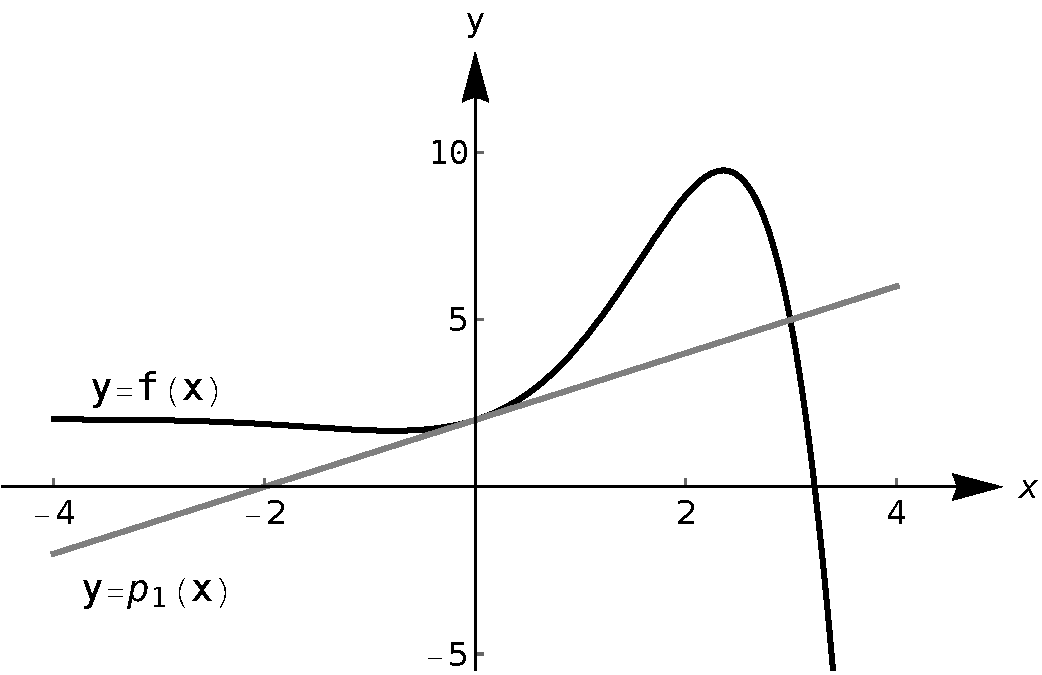
\includegraphics[width=0.45\textwidth]{fig_series_13a}}
\qquad
\subfigure[\label{fig_series_13b}]{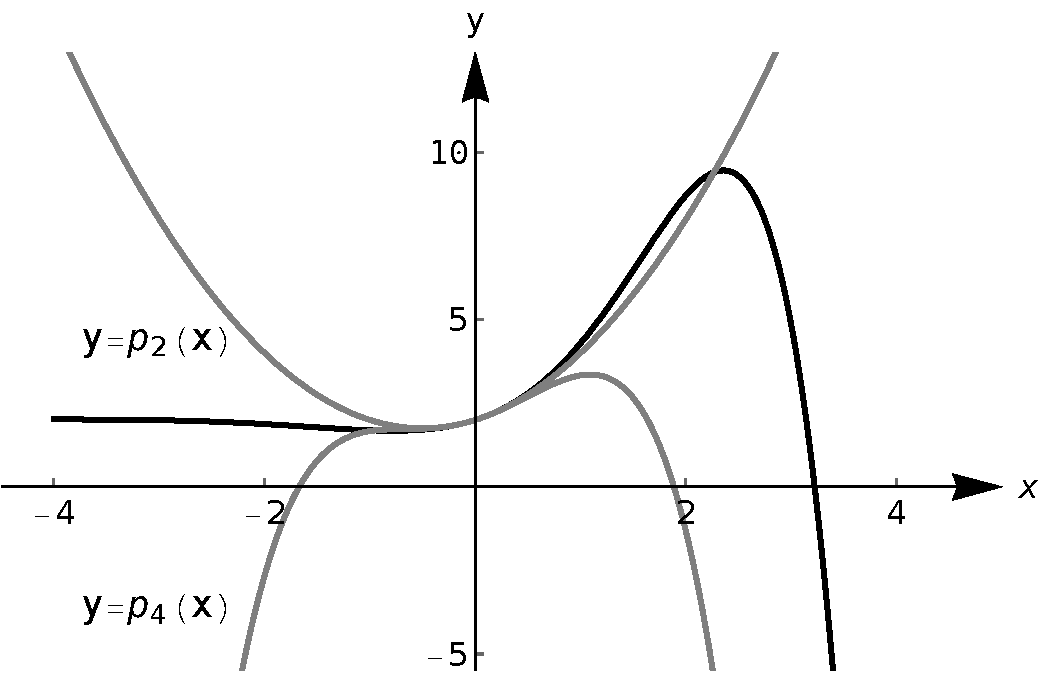
\includegraphics[width=0.45\textwidth]{fig_series_13b} }
\qquad
\subfigure[\label{fig_series_13c}]{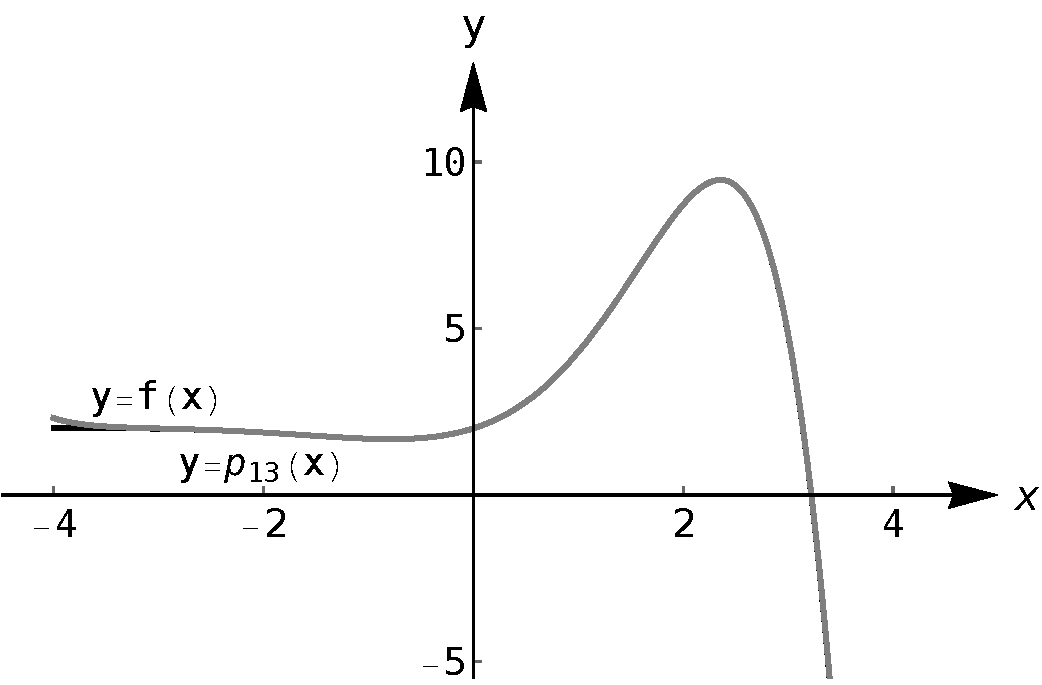
\includegraphics[width=0.45\textwidth]{fig_series_13c} }
\caption{Plotting $f$ and the tangent line at $x=0$ (a) , $f$, $p_2$ and $p_4$ (b), and $f$ and $p_{13}$ (c).}
\end{figure}

We can repeat this approximation process by creating polynomials of higher degree that match more of the derivatives of $f$ at $x=0$. In general, a polynomial of degree $n$ can be created to match the first $n$ derivatives of $f$. Figure \ref{fig_series_13b} also shows $p_4(x)= -x^4/2-x^3/6+x^2+x+2$, whose first four derivatives at 0 match those of $f$. 

As we use more and more derivatives, our polynomial approximation to $f$ gets better and better. In this example, the interval on which the approximation is good gets bigger and bigger. Figure \ref{fig_series_13c} shows $p_{13}(x)$; we can visually affirm that this polynomial approximates $f$ very well on $[-2,3]$. Note, however, that the polynomial $p_{13}(x)$ is not particularly nice. It is \begin{multline*}
p_{13}(x)= \frac{16901x^{13}}{6227020800}+\frac{13x^{12}}{1209600}-\frac{1321x^{11}}{39916800}-\frac{779x^{10}}{1814400}-\frac{359x^9}{362880}+\\
\frac{x^8}{240}+\frac{139x^7}{5040}+\frac{11 x^6}{360}-\frac{19x^5}{120}-\frac{x^4}{2}-\frac{x^3}{6}+x^2+x+2.
\end{multline*}

The polynomials we have created are examples of \textbf{Taylor polynomials} (\textit{Taylor-veelterm}), named after the British mathematician Brook Taylor who made important discoveries about such functions. It can be shown that Taylor polynomials follow a general pattern that make their formation much more direct. This is described in the following definition.

\begin{definition}[Taylor and MacLaurin polynomials]\label{def:taypoly}
Let $f$ be a function whose first $n$ derivatives exist at $x=x_0$.
\index{Taylor polynomial}\index{Maclaurin polynomial} \index[aut]{Taylor polynoom}\index[aut]{MacLaurin polynoom}
\begin{enumerate}
\item		The \textbf{Taylor polynomial of degree $n$ of $f$ at $x=x_0$} is 
				{$$p_n(x) = f(x_0) + \fp(x_0)(x-x_0) + \frac{\fpp(x_0)}{2!}(x-x_0)^2+\frac{\fp''(x_0)}{3!}(x-x_0)^3+\cdots+\frac{f\,^{(n)}(x_0)}{n!}(x-x_0)^n.$$}
\item		A special case of the Taylor polynomial is the Maclaurin polynomial, where $x_0=0$. That is, the \textbf{Maclaurin polynomial of degree $n$ of $f$} is 
{$$p_n(x) = f(0) + \fp(0)x + \frac{\fpp(0)}{2!}x^2+\frac{\fp''(0)}{3!}x^3+\cdots+\frac{f\,^{(n)}(0)}{n!}x^n.$$}
\end{enumerate}
\end{definition}

We will practice creating such polynomials in the following example.

\begin{example}\label{ex_taypoly2}
\begin{enumerate}
\item		Find the $n^\text{th}$ Taylor polynomial of $y=\ln(x)$ at $x=1$.
\item		Use $p_6(x)$ to approximate the value of $\ln(1.5)$.
\item		Use $p_6(x)$ to approximate the value of $\ln(2)$. 
\end{enumerate}

\xhrulefill{gray}{2.5pt}Solution \xhrulefill{gray}{2.5pt}

\begin{enumerate}
\item		We begin by creating a table of derivatives of $\ln (x)$ evaluated at $x=1$. While this is not as straightforward as it was in the previous example, a pattern does emerge, as shown in Table~\ref{tab_series_1}.





Using Definition \ref{def:taypoly}, we have 
\begin{align*}
	p_n(x) &=	f(x_0) + \fp(x_0)(x-x_0) + \frac{\fpp(x_0)}{2!}(x-x_0)^2+\frac{\fp''(x_0)}{3!}(x-x_0)^3+\cdots+\frac{f\,^{(n)}(x_0)}{n!}(x-x_0)^n\\[0.2cm]
					&= 0+(x-1)-\frac12(x-1)^2+\frac13(x-1)^3-\frac14(x-1)^4+\cdots+\frac{(-1)^{n+1}}{n}(x-1)^n.
\end{align*}
\normalsize
Note how the coefficients of the $(x-1)$ terms turn out to be nice.

\begin{table}[H]
\caption{Derivatives of $\ln(x)$ evaluated at $x=1$.}
\label{tab_series_1}
\renewcommand{\arraystretch}{1.5}
\begin{tabular}{c|c}
Derivative function&derivative at $x=1$\\\hline
$f(x) = \ln(x) $&$f(1) = 0$\\%\hline
$\fp(x) = 1/x $&$\fp(1) = 1$\\%\hline
$\fp'(x) = -1/x^2 $&$\fp'(1) = -1$\\%\hline
$\fp''(x) = 2/x^3 $&$\fp''(1) = 2$\\%\hline
$f\,^{(4)}(x) = -6/x^4 $&$f\,^{(4)}(1) = -6$\\%\hline
$\ \vdots $& $\ \vdots$\\%\hline
$f\,^{(n)}(x) = \dfrac{(-1)^{n+1}(n-1)!}{x^n}$ & $f\,^{(n)}(1) = (-1)^{n+1}(n-1)!$\\
%$\ds \rule{0pt}{15pt}\frac{(-1)^{n+1}(n-1)!}{x^n} $ & & $(-1)^{n+1}(n-1)!$\\\hline
\end{tabular}
\renewcommand{\arraystretch}{1}
\end{table}


\item		We can compute $p_6(x)$ using our work above:
$$p_6(x) = (x-1)-\frac12(x-1)^2+\frac13(x-1)^3-\frac14(x-1)^4+\frac15(x-1)^5-\frac16(x-1)^6.$$
Since $p_6(x)$ approximates $\ln(x)$ well near $x=1$, we approximate $\ln(1.5) \approx p_6(1.5)$:

\vspace{-0.5cm}

\begin{align*}
p_6(1.5) &= (1.5-1)-\frac12(1.5-1)^2+\frac13(1.5-1)^3-\frac14(1.5-1)^4+\cdots \\
			&\cdots +\frac15(1.5-1)^5-\frac16(1.5-1)^6\\[0.2cm]
	&=\frac{259}{640}\\[0.2cm]
	&\approx 0.404688.
\end{align*}
\normalsize
This is a good approximation as a calculator shows that $\ln(1.5) \approx 0.4055.$ Figure \ref{fig_series_14a} plots $y=\ln(x)$ with $y=p_6(x)$. We can see that $\ln(1.5)\approx p_6(1.5)$.

\item	
We approximate $\ln(2)$ with $ p_6(2)$:
\begin{align*}
p_6(2) &= (2-1)-\frac12(2-1)^2+\frac13(2-1)^3-\frac14(2-1)^4+\cdots \\
			&\cdots +\frac15(2-1)^5-\frac16(2-1)^6\\
			&=	1-\frac12+\frac13-\frac14+\frac15-\frac16 \\
			&= \frac{37}{60}\\ 
			&\approx 0.616667.
\end{align*}
This approximation is not terribly impressive: a hand held calculator shows that $\ln(2) \approx 0.693147.$ The graph in Figure \ref{fig_series_14a} shows that $p_6(x)$ provides less accurate approximations of $\ln(x)$ as $x$ gets close to 0 or 2. 

Surprisingly enough, even the 20$^\text{th}$ degree Taylor polynomial fails to approximate $\ln(x)$ for $x>2$, as shown in Figure \ref{fig_series_14b}. We will soon discuss why this is.

\end{enumerate}

\begin{figure}[H]
\centering
%\raisebox{0.5cm}{
\subfigure[\label{fig_series_14a}]{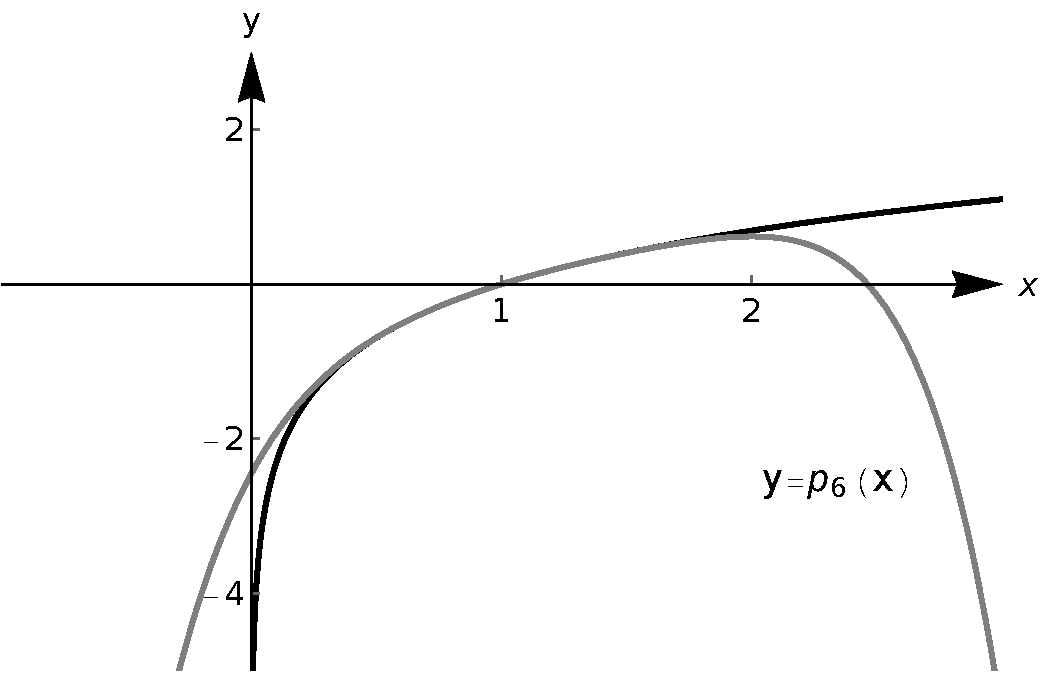
\includegraphics[width=0.45\textwidth]{fig_series_14a}}
\qquad
\subfigure[\label{fig_series_14b}]{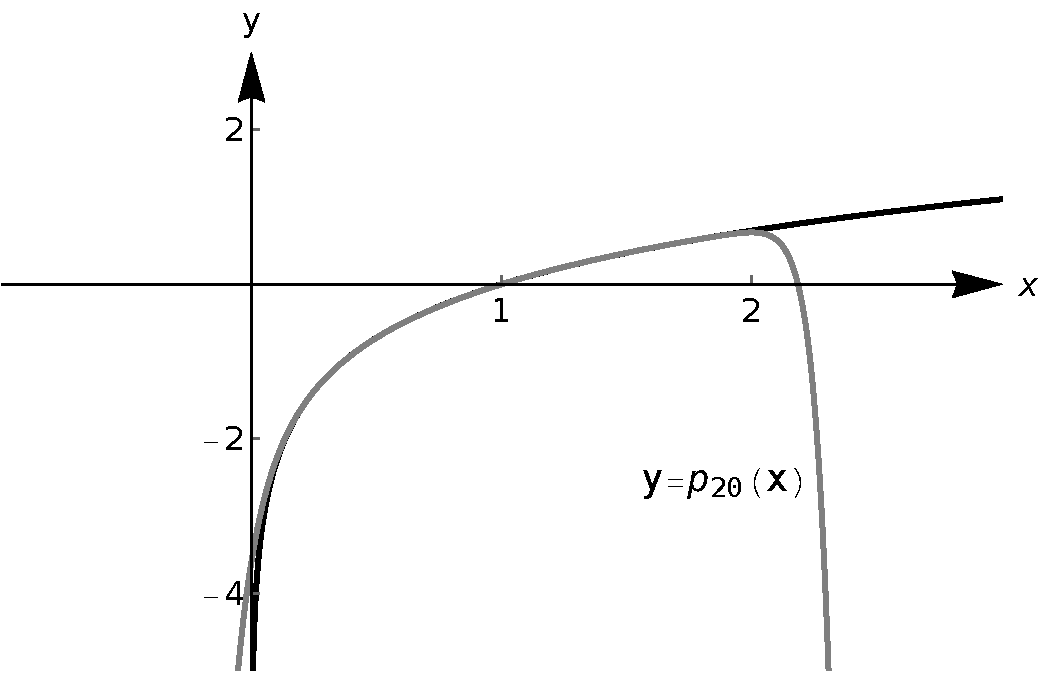
\includegraphics[width=0.45\textwidth]{fig_series_14b} }
\caption{A plot of $y=\ln(x)$ and its 6$^\text{th}$ (a) and  20$^\text{th}$ (b) degree Taylor polynomial at $x=1$.}
\end{figure}


\end{example}


\subsection{Taylor's theorem}

Taylor polynomials are used to approximate functions $f(x)$ in mainly two situations:
	\begin{enumerate}
	\item		When $f(x)$ is known, but perhaps hard to compute directly. For instance, we can define $y=\cos (x)$ as either the ratio of sides of a right triangle or with the unit circle. However, neither of these provides a convenient way of computing $\cos (2)$. A Taylor polynomial of sufficiently high degree can provide a reasonable method of computing such values using only operations usually hard--wired into a computer ($+$, $-$, $\times$ and $\div$).
	
	\item		When $f(x)$ is not known, but information about its derivatives is known. This occurs more often than one might think, especially in the study of differential equations.
	\end{enumerate}
	
In both situations, it is crucial to know how good the approximation is. If we use a Taylor polynomial to compute $\cos (2)$, how do we know how accurate the approximation is? 

 The following theorem provides this kind of information for Taylor (and hence Maclaurin) polynomials.

\begin{theorem}[Taylor's theorem]\label{thm:taylorthm}
\begin{enumerate}
\item	Let $f$ be a function whose $(n+1)^\text{th}$ derivative exists on an interval $I$ and let $x_0$ be in $I$. Then, for each $x$ in $I$, there exists $\theta_x$ between $x$ and $x_0$ such that
\begin{eqnarray*}
f(x) &=&\sum_{i=0}^n\dfrac{f^{(i)}(x_0)}{i!}(x-x_0)^i+\dfrac{f^{(n+1)}(\theta_x)}{(n+1)!}(x-x_0)^{n+1}\\
&=& f(x_0) + \fp(x_0)(x-x_0) + \frac{\fpp(x_0)}{2!}(x-x_0)^2+ \cdots +\frac{f\,^{(n)}(x_0)}{n!}(x-x_0)^n+R_n(x),
\end{eqnarray*}
where $\ds R_n(x) = \frac{f\,^{(n+1)}(\theta_x)}{(n+1)!}(x-x_0)^{(n+1)}$ is the remainder term.
\index{Taylor Polynomial!Taylor's Theorem}\index{Taylor's Theorem}

\item		$\ds \big|R_n(x)\big| \leq \frac{\max\left|\,f\,^{(n+1)}(\theta)\right|}{(n+1)!}\big|(x-x_0)^{(n+1)}\big|$, $ \quad$ where $\theta$ is in $I$.
\end{enumerate}
\end{theorem}

\ifanalysis

\begin{proof}
The proof of the first part of theorem requires some cleverness to set up, but then the details are
quite elementary. We want to define a function $F(t)$. 
Start with the equation
$$F(t)=\sum_{i=0}^n{f^{(i)}(t)\over i!}\,(x-t)^i + B(x-t)^{n+1}.$$
Here we have replaced $x_0$ by $t$ in the first $n+1$ terms of the
Taylor series, and added a carefully chosen term on the end, with $B$
to be determined. Note that
we are temporarily keeping $x$ fixed, so the only variable in this
equation is $t$, and we will be interested
only in $t$ between $x_0$ and $x$. Now substitute $t=x_0$:
$$F(x_0)=\sum_{i=0}^n{f^{(i)}(x_0)\over i!}\,(x-x_0)^i + B(x-x_0)^{n+1}.$$
Set this equal to $f(x)$:
$$f(x)=\sum_{i=0}^n{f^{(i)}(x_0)\over i!}\,(x-x_0)^i + B(x-x_0)^{n+1}.$$
Since $x\not=x_0$, we can solve this for $B$, which is a
``constant''---it depends on $x$ and $x_0$ but those are temporarily 
fixed.  Now we
have defined a function $F(t)$ with the property that
$F(x_0)=f(x)$. Consider also $F(x)$: all terms with a positive power of
$(x-t)$ become zero when we substitute $x$ for $t$, so we are left
with $\ds F(x)=f^{(0)}(x)/0!=f(x)$. So $F(t)$ is a function with the same
value on the endpoints of the interval $[x_0,x]$. 
By Rolle's theorem (\ref{thm:rolles}), we
know that there is a value $z\in(x_0,x)$ such that $F'(z)=0$. Let's look
at $F'(t)$. Each term in $F(t)$, except the first term and the extra
term involving $B$, is a product, so to take the derivative we use the
product rule on each of these terms. It will help to write out the
first few terms of the definition:
$$
  F(t)=f(t)+{f^{(1)}(t)\over 1!}(x-t)^1+{f^{(2)}(t)\over 2!}(x-t)^2+
  {f^{(3)}(t)\over 3!}(x-t)^3+\cdots
  +{f^{(n)}(t)\over n!}(x-t)^n+
  B(x-t)^{n+1}.
$$
Now take the derivative:
\allowdisplaybreaks
\begin{multline*}
  F'(t) = f'(t) + 
  \left({f^{(1)}(t)\over 1!}(x-t)^0(-1)+{f^{(2)}(t)\over
    1!}(x-t)^1\right)\\
  +\left({f^{(2)}(t)\over 1!}(x-t)^1(-1)+{f^{(3)}(t)\over
    2!}(x-t)^2\right)\\
  +\left({f^{(3)}(t)\over 2!}(x-t)^2(-1)+{f^{(4)}(t)\over
    3!}(x-t)^3\right)+\dots+\\
  +\left({f^{(n)}(t)\over (n-1)!}(x-t)^{n-1}(-1)+{f^{(n+1)}(t)\over
    n!}(x-t)^n\right)  +B(n+1)(x-t)^n(-1).
\end{multline*}
Now most of the terms in this expression cancel out,
leaving just
$$F'(t) = {f^{(n+1)}(t)\over n!}(x-t)^n+B(n+1)(x-t)^n(-1).$$
At some $\theta_x$, $F'(z_x)=0$ so
$$
  0={f^{(n+1)}(\theta_x)\over n!}(x-\theta_x)^n+B(n+1)(x-\theta_x)^n(-1)
$$
from which
$$
  B(n+1)(x-\theta_x)^n={f^{(n+1)}(\theta_x)\over n!}(x-\theta_x)^n
$$
and finally
$$
  B={f^{(n+1)}(\theta_x)\over (n+1)!}.
$$

Now we can write 
$$
  F(t)=\sum_{i=0}^n{f^{(i)}(t)\over i!}\,(x-t)^i + 
  {f^{(n+1)}(\theta_x)\over (n+1)!}(x-t)^{n+1}.
$$
Recalling that $F(x_0)=f(x)$ we get
$$
  f(x)=\sum_{i=0}^n{f^{(i)}(x_0)\over i!}\,(x-x_0)^i + 
  {f^{(n+1)}(\theta_x)\over (n+1)!}(x-x_0)^{n+1},
$$
which is what we wanted to show.

For what concerns the second part, it is clear that if you find an upper bound $M$  on the absolute value of the $(n+1)$-st derivative of $f$ between $x_0$ and $x$, then the error can be at most
$$
\ds \big|R_n(x)\big| \leq \frac{M}{(n+1)!}\big|(x-x_0)^{(n+1)}\big|
$$
\end{proof}

\fi

Basically, the first part of Taylor's theorem states that $f(x) = p_n(x) + R_n(x)$, where $p_n(x)$ is the $n^\text{th}$ order Taylor polynomial and $R_n(x)$ is the remainder, or error, in the Taylor approximation. The second part gives bounds on how big that error can be. If the $(n+1)^\text{th}$ derivative is large on $I$, the error may be large; if $x$ is far from $x_0$, the error may also be large. However, the $(n+1)!$ term in the denominator tends to ensure that the error gets smaller as $n$ increases.




%\ifanalysis
%
%Andere vormen resttermen Taylor: Bron zie code
%http://www.stewartcalculus.com/data/CALCULUS%20Early%20Transcendentals/upfiles/Formulas4RemainderTaylorSeries5ET.pdf
%VRAAG: nemen we die op of niet? 
%
%\fi

The following example computes error estimates for the approximations of $\ln(1.5)$ and $\ln(2)$ made in Example \ref{ex_taypoly2}.

\begin{example}\label{ex_taypoly3}
Find error bounds when approximating 1) $\ln(1.5)$ and 2) $\ln(2)$ with $p_6(x)$, the Taylor polynomial of degree 6 of $f(x)=\ln(x)$ at $x=1$, as calculated in Example \ref{ex_taypoly2}. 

\pagebreak
\xhrulefill{gray}{2.5pt}Solution \xhrulefill{gray}{2.5pt}

\begin{enumerate}
\item	We start with the approximation of $\ln(1.5)$ with $p_6(1.5)$. The theorem references an open interval $I$ that contains both $x$ and $x_0$. The smaller the interval we use the better; it will give us a more accurate (and smaller!) approximation of the error. We let $I = \left.\right]0.9,1.6\left[\right.$, as this interval contains both $c=1$ and $x=1.5$. 

The theorem references $\max\big|f\,^{(n+1)}(\theta)\big|$. In our situation, this is asking the question how big can the $7^\text{th}$ derivative of $y=\ln(x)$ be on the interval $]0.9,1.6[$. The seventh derivative is $y = -6!/x^7$. The largest value it attains on $I$ is about 1506. Thus we can bound the error as:
\begin{align*}
\big|R_6(1.5)\big| &\leq \frac{\max\big|f\,^{(7)}(\theta)\big|}{7!}\big|(1.5-1)^7\big|\\
					&\leq \frac{1506}{5040}\cdot\frac1{2^7}\\
					&\approx 0.0023.
\end{align*}
\noindent%\drawexampleline
We computed $p_6(1.5) = 0.404688$; using a calculator, we find $\ln(1.5) \approx 0.405465$, so the actual error is about $0.000778$, which is less than our bound of $0.0023$. This affirms Taylor's theorem.

\item		We again find an interval $I$ that contains both $c=1$ and $x=2$; we choose $I = \left.\right]0.9,2.1\left[\right.$. The maximum value of the seventh derivative of $f$ on this interval is again about 1506 (as the largest values come near $x=0.9$). Thus 
\begin{align*}
\big| R_6(2)\big| &\leq \frac{\max\big|f\,^{(7)}(\theta)\big|}{7!}\big|(2-1)^7\big|\\
					&\leq \frac{1506}{5040}\cdot1^7\\
					&\approx 0.30.
\end{align*}
This bound is not as nearly as good as before. Using the degree 6 Taylor polynomial at $x =1$ will bring us within 0.3 of the correct answer. As $p_6(2)\approx 0.61667$, our error estimate guarantees that the actual value of $\ln(2)$ is somewhere between $0.31667$ and $0.91667$. These bounds are not particularly useful.

In reality, our approximation was only off by about 0.07. However, we are approximating ostensibly because we do not know the real answer. In order to be assured that we have a good approximation, we would have to resort to using a polynomial of higher degree.
\end{enumerate}
\end{example}

We may also use Taylor's theorem to find $n$ that guarantees our approximation is within a certain amount.

\begin{example}\label{ex_taypoly4}
Find $n$ such that the $n^\text{th}$ Taylor polynomial of $f(x)=\cos(x)$ at $x=0$ approximates $\cos(2)$ to within $0.001$ of the actual answer. What is $p_n(2)$?

\xhrulefill{gray}{2.5pt}Solution \xhrulefill{gray}{2.5pt}

Following Taylor's theorem, we need bounds on the size of the derivatives of $f(x)=\cos(x)$. In the case of this trigonometric function, this is easy. All derivatives of cosine are $\pm \sin(x)$ or $\pm \cos(x)$. In all cases, these functions are never greater than 1 in absolute value. We want the error to be less than $0.001$. To find the appropriate $n$, consider the following inequalities:
\begin{align*}
\frac{\max\big|f\,^{(n+1)}(\theta)\big|}{(n+1)!}\big|(2-0)^{(n+1)}\big| &\leq 0.001 \\
\Leftrightarrow\quad\frac1{(n+1)!}\cdot2^{(n+1)} &\leq 0.001
\end{align*}
We find an $n$ that satisfies this last inequality with trial--and--error. When $n=8$, we have $\ds \frac{2^{8+1}}{(8+1)!} \approx 0.0014$; when $n=9$, we have $\ds \frac{2^{9+1}}{(9+1)!} \approx 0.000282 <0.001$. Thus we want to approximate $\cos(2)$ with $p_9(2)$.\\

We now set out to compute $p_9(x)$. We again need a table of the derivatives of $f(x)=\cos(x)$ evaluated at $x=0$ (Table~\ref{tab_series_2}).

\begin{table}[H]
\caption{The derivatives of $f(x)=\cos(x)$ evaluated at $x=0$.}
\label{tab_series_2}
\renewcommand{\arraystretch}{1.5}
\begin{tabular}{c|c}
Derivative function&derivative at $x=0$\\\hline
$f(x) = \cos (x) $&$f(0) = 1$\\
$\fp(x) = -\sin (x) $&$\fp(0) = 0$\\
$\fp'(x) = -\cos (x) $&$\fp'(0) = -1$\\
$\fp''(x) = \sin (x) $&$\fp''(0) = 0$\\
$f\,^{(4)}(x) = \cos (x) $&$f\,^{(4)}(0) = 1$\\
$f\,^{(5)}(x) = -\sin (x) $&$f\,^{(5)}(0) = 0$\\
$f\,^{(6)}(x) = -\cos (x) $&$f\,^{(6)}(0) = -1$\\
$f\,^{(7)}(x) = \sin (x) $&$f\,^{(7)}(0) = 0$\\
$f\,^{(8)}(x) = \cos (x) $&$f\,^{(8)}(0) = 1$\\
$f\,^{(9)}(x) = -\sin (x) $&$f\,^{(9)}(0) = 0$\\
\end{tabular}
\renewcommand{\arraystretch}{1}
\end{table}


Notice how the derivatives, evaluated at $x=0$, follow a certain pattern. All the odd powers of $x$ in the Taylor polynomial will disappear as their coefficient is 0. While our error bounds state that we need $p_9(x)$, our work shows that this will be the same as $p_8(x)$. 

Since we are forming our polynomial at $x=0$, we are creating a Maclaurin polynomial, and:
\begin{align*}
p_8(x) &= f(0) + \fp(0)x + \frac{\fpp(0)}{2!}x^2 + \frac{\fp''(0)}{3!}x^3 + \cdots +\frac{f\,^{(8)}(0)}{8!}x^8\\
		&=  1-\frac{1}{2!}x^2+\frac{1}{4!}x^4-\frac{1}{6!}x^6+\frac{1}{8!}x^8
\end{align*}

We finally approximate $\cos(2)$:
$$\cos(2) \approx p_8(2) = -\frac{131}{315} \approx -0.41587.$$ Our error bound guarantee that this approximation is within $0.001$ of the correct answer. Technology shows us that our approximation is actually within about $0.0003$ of the correct answer.
Figure \ref{fig_series_15} shows a graph of $y=p_8(x)$ and $y=\cos(x)$. Note how well the two functions agree on about $\left.\right]-\pi,\pi\left[\right.$.


\begin{figure}[H]
	\begin{center}
			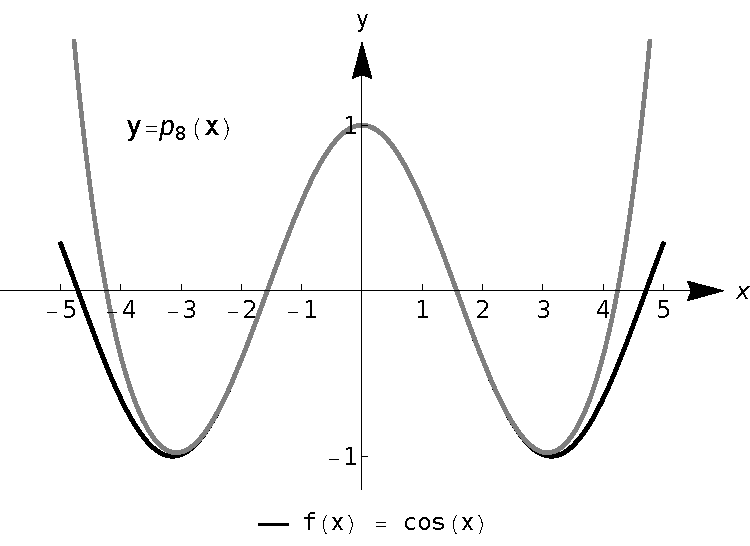
\includegraphics[width=0.5\textwidth]{fig_series_15}
	\caption{A graph of $f(x)= \cos(x)$ (black) and its degree 8 Maclaurin polynomial (gray).}
	\label{fig_series_15}
	\end{center}
\end{figure}

\end{example}


Most of this chapter has been devoted to the study of infinite series. This section has taken a step back from this study, focusing instead on finite summation of terms. In the next section, we explore Taylor series, where we represent a function with an infinite series.

\section{Taylor series}\label{sec:taylor_series}

In Section \ref{sec:power_series}, we showed how certain functions can be represented by a power series function. In Section \ref{sec:taylor_poly}, we showed how we can approximate functions with polynomials, given that enough derivative information is available. In this section we combine these concepts: if a function $f(x)$ is infinitely differentiable, we show how to represent it with a power series function.

\begin{definition}[Taylor and Maclaurin series]\label{def:taylor_series}
Let $f(x)$ have derivatives of all orders at $x=x_0$.
\index{Taylor series}\index{Maclaurin series}\index[aut]{Maclaurin reeks}\index[aut]{Taylor reeks}\index{series!Taylor}\index{series!Maclaurin}\index[aut]{reeks ! Taylor}\index[aut]{reeks ! Maclaurin}
\begin{enumerate}
	\item The \textbf{Taylor series of $f(x)$} (\textit{Taylor-reeks}), centred at $x_0$ is
	$$\sum_{n=0}^{+\infty} \frac{f\,^{(n)}(x_0)}{n!}(x-x_0)^n.$$
	\item	Setting $x_0=0$ gives the \textbf{Maclaurin series of $f(x)$} (\textit{Maclaurin-reeks}):
	$$\sum_{n=0}^{+\infty} \frac{f\,^{(n)}(0)}{n!}x^n.$$
\end{enumerate}
\end{definition}

Note that the order of a Taylor series is determined by the highest-order derivative that appears in it. So the third-order Taylor series expansion of a function $f$ contains terms up to those containing $x^3$.  If $p_n(x)$ is the $n^\text{th}$ degree Taylor polynomial for $f(x)$ centred at $x=x_0$, we saw how $f(x)$ is approximately equal to $p_n(x)$ near $x=x_0$. We also saw how increasing the degree of the polynomial generally reduced the error. We are now considering series, where we sum an infinite set of terms. Our ultimate hope is to see the error vanish and claim a function is equal to its Taylor series.\index{order}\index[aut]{orde}


When creating the Taylor polynomial of degree $n$ for a function $f(x)$ at $x=x_0$, we needed to evaluate $f$, and the first $n$ derivatives of $f$, at $x=x_0$. When creating the Taylor series of $f$, it helps to find a pattern that describes the $n^\text{th}$ derivative of $f$ at $x=x_0$. We demonstrate this in the next example.

\begin{example}\label{ex_ts2}
Find the Taylor series of $f(x) = \ln(x)$ centred at $x=1$.

\xhrulefill{gray}{2.5pt}Solution \xhrulefill{gray}{2.5pt}

Table \ref{tab_series_4} shows the $n^\text{th}$ derivative of $\ln(x)$ evaluated at $x=1$ for $n=0,\ldots,5$, along with an expression for the $n^\text{th}$ term: $$f\,^{(n)}(1) = (-1)^{n+1}(n-1)!\quad \text{for $n\geq 1$.}$$ Remember that this is what distinguishes Taylor series from Taylor polynomials; we are very interested in finding a pattern for the $n^\text{th}$ term, not just finding a finite set of coefficients for a polynomial.

\begin{table}[H]
\caption{The derivatives of $\ln(x)$ evaluated at $x=1$.}
\label{tab_series_4}
\renewcommand{\arraystretch}{1.5}
\begin{tabular}{c|c}
Derivative function&derivative at $x=1$\\\hline
$f(x) = \ln(x) $&$f(1) = 0$\\
$\fp(x) = 1/x $&$\fp(1) = 1$\\
$\fp'(x) = -1/x^2 $&$\fp'(1) = -1$\\
$\fp''(x) = 2/x^3 $&$\fp''(1) = 2$\\
$f\,^{(4)}(x) = -6/x^4 $&$f\,^{(4)}(1) = -6$\\
$f\,^{(5)}(x) = 24/x^5 $&$f\,^{(5)}(1) = 24$\\
$\ \vdots $& $\ \vdots$\\
$f\,^{(n)}(x) = \frac{(-1)^{n+1}(n-1)!}{x^n}$ & $f\,^{(n)}(1) = (-1)^{n+1}(n-1)!$\\
\end{tabular}
\renewcommand{\arraystretch}{1}
\end{table}


Since $f(1) = \ln(1) = 0$, we skip the first term and start the summation with $n=1$, giving the Taylor series for $\ln(x)$, centred at $x=1$, as 
$$\sum_{n=1}^{+\infty} (-1)^{n+1}(n-1)!\frac{1}{n!}(x-1)^n = \sum_{n=1}^{+\infty} (-1)^{n+1}\frac{(x-1)^n}{n}. $$
We now determine the interval of convergence, using the ratio test.
\begin{align*}
\lim_{n\to+\infty} \left|(-1)^{n+2}\frac{(x-1)^{n+1}}{n+1}\right|\Bigg/\left|(-1)^{n+1}\frac{(x-1)^n}{n}\right| &= \lim_{n\to+\infty} \left|\frac{(x-1)^{n+1}}{(x-1)^n}\right|\frac{n}{n+1}\\[0.2cm]
&= \big|(x-1)\big|.
\end{align*}
By the ratio test, we have convergence when $\big|(x-1)\big| <1$: the radius of convergence is 1, and we have convergence on $\left.\right]0,2\left[\right.$. We now check the endpoints.

At $x=0$, the series is 
$$\sum_{n=1}^{+\infty} (-1)^{n+1}\frac{(-1)^n}{n} = -\sum_{n=1}^{+\infty} \frac1n,$$
which diverges as it is the harmonic series times $(-1)$.

At $x=2$, the series is
$$\sum_{n=1}^{+\infty} (-1)^{n+1}\frac{(1)^n}{n} = \sum_{n=1}^{+\infty} (-1)^{n+1}\frac{1}{n},$$
the alternating harmonic series, which converges conditionally.


We have found the Taylor series of $\ln (x)$ centred at $x=1$, and have determined the series converges on $\left.\right]0,2]$. We cannot (yet) say that $\ln (x)$ is equal to this Taylor series on $\left.\right]0,2]$.
\end{example}

\ifmathematica
Also in Mathematica it is possible to determine the \textbf{series expansion} (\textit{reeks-ontwikkeling}) of a function. For instance, to get the Taylor series of $f(x) = \ln(x)$ centred at $x=1$, we can proceed as follows with the command \lstinline{Series}. 
	\begin{mdframed}[default,backgroundcolor=gray!40,roundcorner=8pt]
\begin{mmaCell}[morefunctionlocal={x}]{Input}
  Series[Log[x],\{x,1,5\}]
\end{mmaCell}

\begin{mmaCell}{Output}
  (x-1)-\mmaFrac{1}{2} \mmaSup{(x-1)}{2}+\mmaFrac{1}{3} \mmaSup{(x-1)}{3}-\mmaFrac{1}{4} \mmaSup{(x-1)}{4}+\mmaFrac{1}{5} \mmaSup{(x-1)}{5}+\mmaSup{O[x-1]}{6}
\end{mmaCell}
\end{mdframed}
The general syntax of this command is 
\begin{mmaCell}[morefunctionlocal={x}]{Input}
  Series[f[x],\{x,x0,n\},]
\end{mmaCell}
where \lstinline{f[x]} is the function at stake, \lstinline{x} the variable, \lstinline{x0} the point at which the series is centred and \lstinline{n} the order. 
\fi

\ifpython
Also in Python it is possible to determine the \textbf{series expansion} (\textit{reeks-ontwikkeling}) of a function. For instance, to get the Taylor series of $f(x) = \ln(x)$ centred at $x=1$, we can proceed as follows with the command \lstinline{series}. 
\begin{pyin}
from sympy import symbols, series, ln
x = symbols('x')
series(ln(x),x,1,6)
\end{pyin}
\begin{pyout}
-1 - \frac{(x-1)^2}{2} + \frac{(x-1)^3}{3} - \frac{(x-1)^4}{4} + \frac{(x-1)^5}{5} + x + \mathcal{O}((x-1)^6; x\rightarrow 1)
\end{pyout}
The general syntax of this command is 
\begin{pyin}
series(f(x),x,x0,n)
\end{pyin}
where \lstinline{f[x]} is the function at stake, \lstinline{x} the variable, \lstinline{x0} the point at which the series is centred and \lstinline{n} the order.
\fi

It is important to note that Definition \ref{def:taylor_series} defines a Taylor series given a function $f(x)$, but makes no claim about their equality.  We will find that most of the time they are equal, but we need to consider the conditions that allow us to conclude this.

Theorem \ref{thm:taylorthm} states that the error between a function $f(x)$ and its $n^\text{th}$--degree Taylor polynomial $p_n(x)$ is $R_n(x)$, where
$$ \big|R_n(x)\big| \leq \frac{\max\left|\,f\,^{(n+1)}(\theta)\right|}{(n+1)!}\big|(x-x_0)^{(n+1)}\big|.$$

If $R_n(x)$ goes to 0 for each $x$ in an interval $I$ as $n$ approaches infinity, we conclude that the function is equal to its Taylor series expansion. This formalized in the following theorem. 

\begin{theorem}[Function and Taylor series equality]\label{thm:function_series_equality}
Let $f(x)$ have derivatives of all orders at $x=x_0$ i.e. $f(x)$ is a smooth function, let $R_n(x)$ be as stated in Theorem \ref{thm:taylorthm}, and let $I$ be an interval on which the Taylor series of $f(x)$ converges. 
If $\ds\lim_{n\to+\infty} R_n(x) = 0$ for all $x$ in $I$, then 
$$f(x) = \sum_{n=0}^{+\infty} \frac{f\,^{(n)}(x_0)}{n!}(x-x_0)^n\;  \text{on $I$}. $$
\end{theorem}

\ifanalysis

\begin{proof}
This theorem is an immediate consequence of Theorem~\ref{thm:taylorthm}. 
\end{proof}
We demonstrate the use of this theorem in an example.\\

\begin{example}\label{ex_ts3}
Show that $f(x) = \cos(x)$ is equal to its Maclaurin series, given by
$$
\sum_{n=0}^{+\infty} (-1)^{n}\frac{x^{2n}}{(2n)!},
$$
for all $x$. 

\xhrulefill{gray}{2.5pt}Solution \xhrulefill{gray}{2.5pt}

Given a value $x$, the magnitude of the error term $R_n(x)$ is bounded by
$$ \big|R_n(x)\big| \leq \frac{\max\left|\,f\,^{(n+1)}(\theta)\right|}{(n+1)!}\big|x^{n+1}\big|.$$
Since all derivatives of $\cos x$ are $\pm \sin x$ or $\pm\cos x$, whose magnitudes are bounded by $1$, we can state
$$ \big|R_n(x)\big| \leq \frac{1}{(n+1)!}\big|x^{n+1}\big|$$
which implies
\begin{equation}
 -\frac{|x^{n+1}|}{(n+1)!} \leq R_n(x) \leq\frac{|x^{n+1}|}{(n+1)!}.\label{eq:coseqtaylor}
\end{equation}
For any $x$, $\ds\lim_{n\to+\infty} \frac{x^{n+1}}{(n+1)!} = 0$. Applying the squeeze theorem to Equation \eqref{eq:coseqtaylor}, we conclude that $\ds \lim_{n\to+\infty} R_n(x) = 0$ for all $x$, and hence
$$\cos (x) = \sum_{n=0}^{+\infty} (-1)^{n}\frac{x^{2n}}{(2n)!}\quad \text{for all $x$}.$$
\end{example}

\fi

It is natural to assume that a function is equal to its Taylor series on the series' interval of convergence, but this is not always the case. In order to properly establish equality, one must use Theorem \ref{thm:function_series_equality}. This is a bit disappointing, as we developed beautiful techniques for determining the interval of convergence of a power series, and proving that $R_n(x)\to 0$ can be difficult. For instance, it is not a simple task to show that $\ln (x)$ equals  its Taylor series on $\left.\right]0,2]$ as found in Example \ref{ex_ts2}.
%cumbersome as it deals with high order derivatives of the function. (In the Exercises, proof of equality is sometimes limited

\begin{remark}[Fourier series]
A Fourier series is another kind of series that is used to represent a function as the sum of simple sine waves. Essentially, it decomposes any periodic function  into the sum of a (possibly infinite) set of simple oscillating functions, namely sines and cosines. The Fourier series has many  applications in electrical engineering, vibration analysis, acoustics, optics, signal processing, image processing, quantum mechanics, econometrics, and so on. Figure~\ref{fig_series_16} shows the Fourier series approximation of a square wave using 5 and 15 terms. 

\begin{figure}[H]
	\begin{center}
			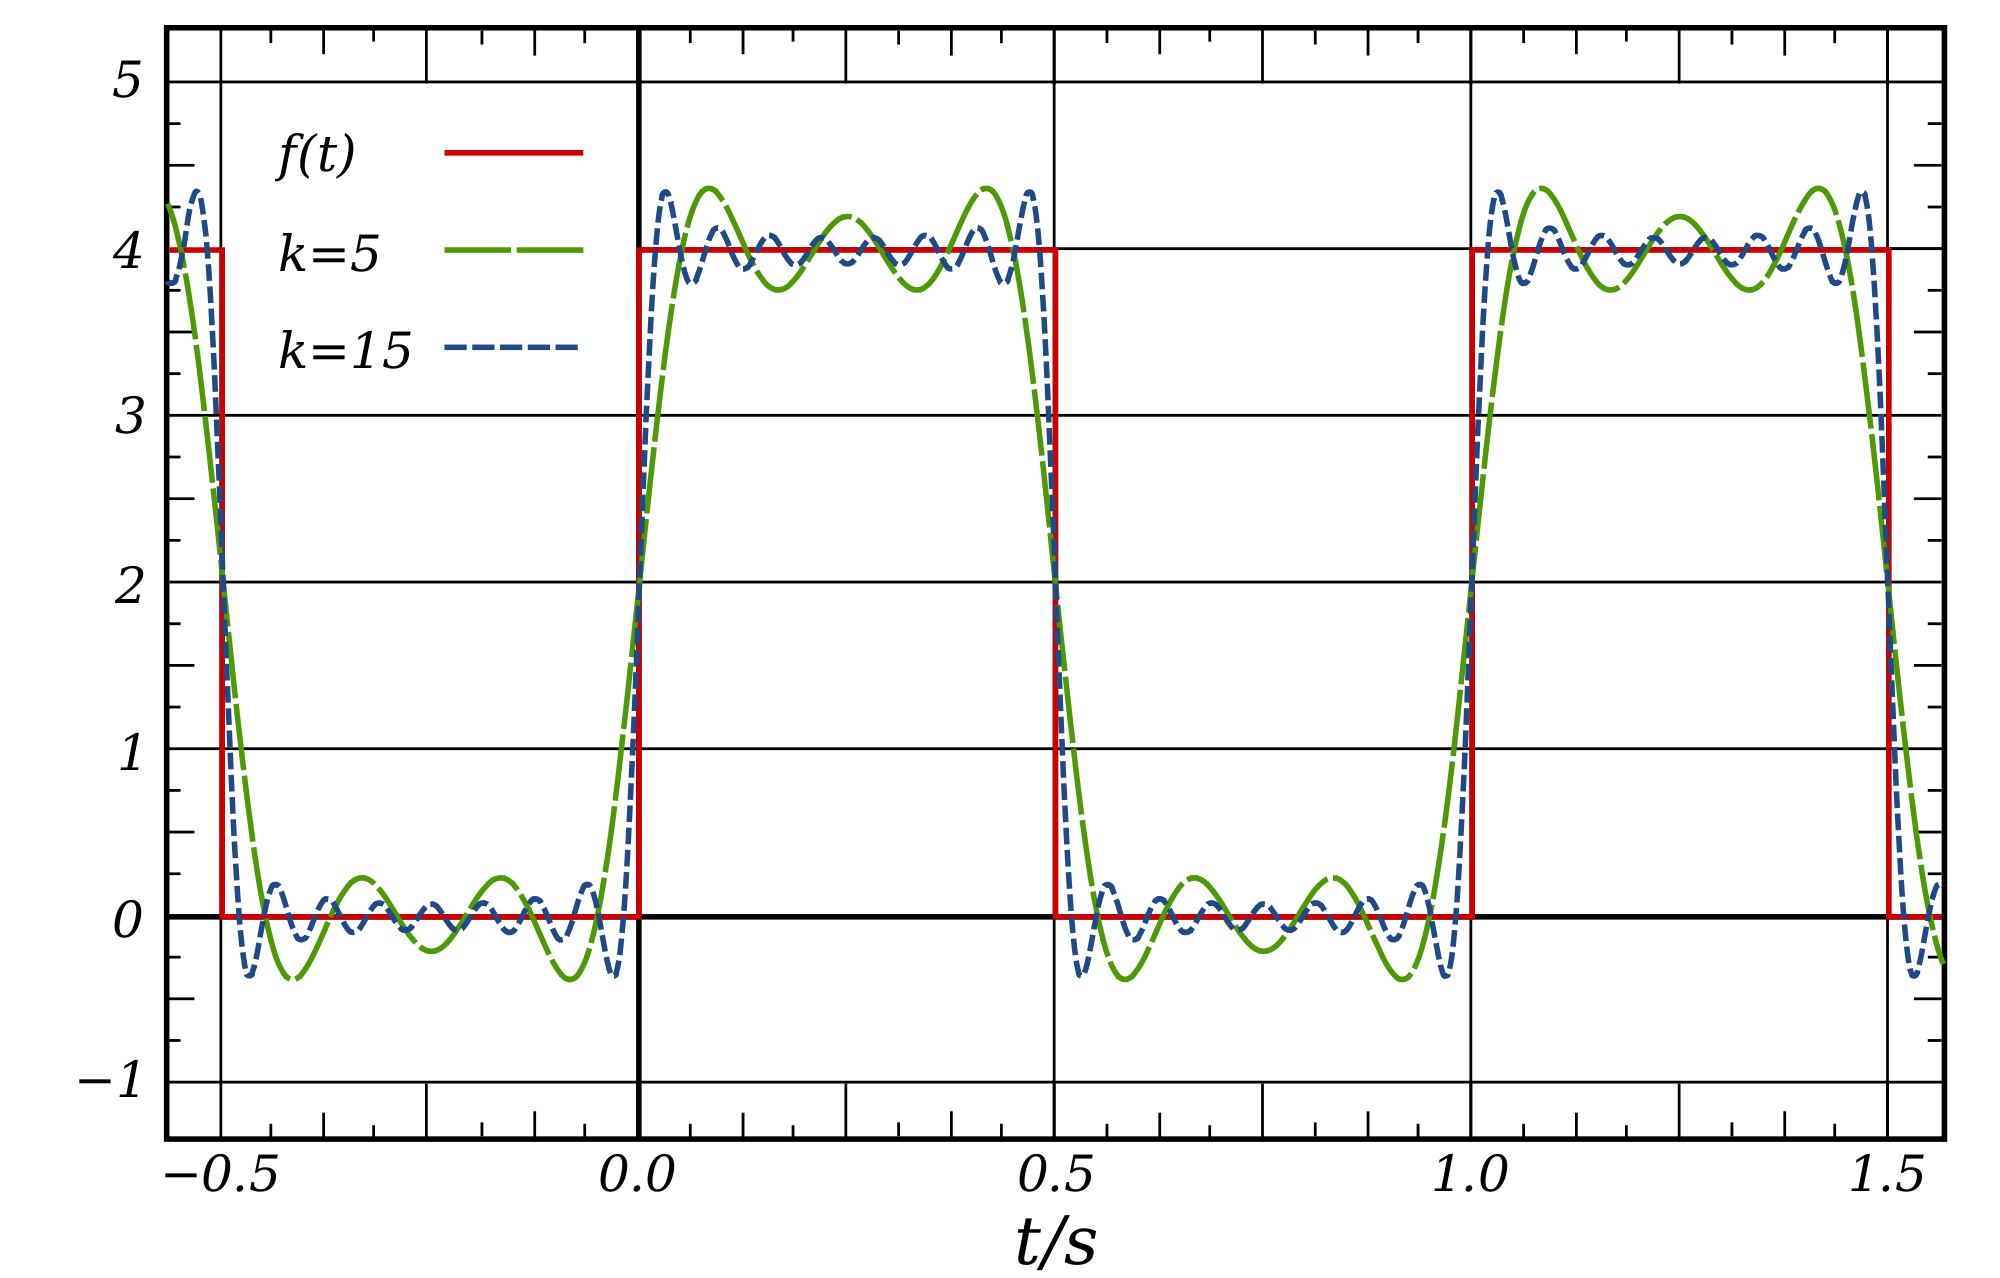
\includegraphics[width=0.5\textwidth]{fig_series_16}
	\caption{ Fourier series approximation of a square wave using 5 and 15 terms.}
	\label{fig_series_16}
	\end{center}
\end{figure}


\end{remark}

A function $f(x)$ that is equal to its Taylor series, centered at any point of the domain of $f(x)$, is said to be an \textbf{analytic function} (\textit{analytische functie}),\index{analytic function}\index[aut]{functie ! analytisch}\index[aut]{analytische functie} and most functions that we will encounter are analytic functions. Generally speaking, any function that one creates with elementary functions (polynomials, exponentials, trigonometric functions, etc.) that is not piecewise defined is probably analytic. For most functions, we may assume the function is equal to its Taylor series on the series' interval of convergence and only use Theorem \ref{thm:function_series_equality} when we suspect something may not work as expected.

We develop the Taylor series for one more important function, then give a table of the Taylor series for a number of common functions.\index{binomial series}\index{series!binomial}\index[aut]{reeks ! binomiaal}

\begin{example}\label{ex_ts4}
Find the Maclaurin series of $f(x) = (1+x)^k$ with $k\neq 0$.

\xhrulefill{gray}{2.5pt}Solution \xhrulefill{gray}{2.5pt}

When $k$ is a positive integer, the Maclaurin series is finite. For instance, when $k=4$, we have 
$$f(x) = (1+x)^4 = 1+4x+6x^2+4x^3+x^4.$$
The coefficients of $x$ when $k$ is a positive integer are known as the binomial coefficients, giving the series we are developing its name.
When $k=1/2$, we have $f(x) = \sqrt{1+x}$. Knowing a series representation of this function would give a useful way of approximating $\sqrt{1.3}$, for instance.
To develop the Maclaurin series for $f(x) = (1+x)^k$ for any value of $k\neq0$, we consider the derivatives of $f$ evaluated at $x=0$ as in Table \ref{tab_series_3}

%\noindent\hskip-30pt\begin{minipage}{1.3\linewidth}
%\begin{align*}
\begin{table}[H]
\caption{The derivatives of $f(x) = (1+x)^k$ evaluated at $x=0$.}
\label{tab_series_3}
\renewcommand{\arraystretch}{1.5}
\begin{tabular}{c|c}
Derivative function&derivative at $x=0$\\\hline
$f(x) = (1+x)^k$ & $f(0) = 1$\\
$\fp(x) = k(1+x)^{k-1} $&$ \fp(0) =k$\\
$\fp'(x) = k(k-1)(1+x)^{k-2}$ & $\fp'(0) =k(k-1)$\\
$\fp''(x) = k(k-1)(k-2)(1+x)^{k-3}$ & $\fp''(0) =k(k-1)(k-2)$\\
$\vdots$ & $\vdots$\\
$f\,^{(n)}(x) = k(k-1)\cdots\big(k-(n-1)\big)(1+x)^{k-n}$ & $f\,^{(n)}(0) =k(k-1)\cdots\big(k-(n-1)\big)$\\\hline
\end{tabular}
\renewcommand{\arraystretch}{1}
\end{table}
%\end{align*}
%\end{minipage}

Thus the Maclaurin series for $f(x) = (1+x)^k$ is
$$1+ kx + \frac{k(k-1)}{2!}x^2 + \frac{k(k-1)(k-2)}{3!}x^3 + \ldots + \frac{k(k-1)\cdots\big(k-(n-1)\big)}{n!}x^n+\ldots\,.$$

It is important to determine the interval of convergence of this series. With 
$$a_n = \frac{k(k-1)\cdots\big(k-(n-1)\big)}{n!}x^n,$$
we apply the ratio test:
\begin{align*}
\lim_{n\to+\infty}\frac{|a_{n+1}|}{|a_n|}&=\lim_{n\to+\infty} \left|\frac{k(k-1)\cdots(k-n)}{(n+1)!}x^{n+1}\right|\Bigg/\left|\frac{k(k-1)\cdots\big(k-(n-1)\big)}{n!}x^n\right|\\
		&=\lim_{n\to+\infty} \left|\frac{k-n}{n+1}x\right|\\
		&= |x|.
\end{align*}

The series converges absolutely when the limit of the ratio test is less than 1; therefore, we have absolute convergence when $|x|<1$. 

It can be verified that the interval of convergence depends on the value of $k$. When $k>0$, the interval of convergence is $[-1,1]$. When $-1<k<0$, the interval of convergence is $]-1,1]$. If $k\leq -1$, the interval of convergence is $\left.\right]-1,1\left[\right.$.

\end{example}

We learned that Taylor polynomials offer a way of approximating a difficult to compute function with a polynomial. Taylor series offer a way of exactly representing a function with a series. One probably can see the use of a good approximation; is there any use of representing a function exactly as a series? Yes, amongst other things they provide a valuable tool for solving a variety of problems, including problems relating to integration and differential equations. 

In Table~\ref{idea:common_taylor} we give  the Taylor series of a number of common functions. 

\begin{table}
\caption{Important Taylor series expansions.}
\label{idea:common_taylor}
\begin{tabular}{l|l|c}
Function and Series & First few terms & \parbox{50pt}{\centering Interval of\\convergence} \\\hline
\rule{0pt}{25pt}$\ds e^x = \sum_{n=0}^{+\infty} \frac{x^n}{n!}$ & $\ds 1+ x+\frac{x^2}{2!} + \frac{x^3}{3!}+\cdots$ & $\mathbb{R} $\\
\rule{0pt}{25pt}$\ds \sin(x) = \sum_{n=0}^{+\infty} (-1)^n\frac{x^{2n+1}}{(2n+1)!}$ & $\ds x-\frac{x^3}{3!}+\frac{x^5}{5!} - \frac{x^7}{7!}+\cdots$ & $\mathbb{R}$\\
\rule{0pt}{25pt}$\ds \cos(x) = \sum_{n=0}^{+\infty} (-1)^n\frac{x^{2n}}{(2n)!}$ & $\ds 1-\frac{x^2}{2!}+\frac{x^4}{4!} - \frac{x^6}{6!} +\cdots$ & $\mathbb{R}$\\
\rule{0pt}{25pt}$\ds \ln(x) = \sum_{n=1}^{+\infty}(-1)^{n+1}\frac{(x-1)^n}{n}$ & $\ds (x-1)- \frac{(x-1)^2}{2} +\frac{(x-1)^3}{3}-\cdots$& $]0,2]$\\
\rule{0pt}{25pt}$\ds \frac{1}{1-x} = \sum_{n=0}^{+\infty} x^n$ &$\ds 1+x+x^2+x^3+\cdots$& $[-1,1[$\\
\rule{0pt}{25pt}$\ds (1+x)^k=\sum_{n=0}^{+\infty} \frac{k(k-1)\cdots\big(k-(n-1)\big)}{n!}x^n$ & $\ds 1+kx+\frac{k(k-1)}{2!}x^2 + \cdots$ & $]-1,1[$\footnote{Convergence at $x=\pm1$ depends on the value of $k$.}\\
\rule{0pt}{25pt}$\ds \arctan(x) = \sum_{n=0}^{+\infty} (-1)^n\frac{x^{2n+1}}{2n+1}$ & $\ds x-\frac{x^3}{3}+\frac{x^5}{5}-\frac{x^7}{7}+\cdots$ & $[-1,1]$\\
\end{tabular}
\end{table}

We also give a theorem about the algebra of power series, that is, how we can combine power series to create power series of new functions. This allows us to find the Taylor series of functions like $f(x) = e^x\cos (x)$ by knowing the Taylor series of $e^x$ and $\cos (x)$.


	\checkoddpage
\marginpar{\ifoddpage\hspace*{-1.5cm}\else\hspace*{0.25cm}\fi
\includegraphics[width=0.075\textwidth]{youtube}\\
\ifoddpage\hspace*{-1.75cm}\else\hspace*{0.1cm}\fi
\qrcode[height=1.75cm]{https://youtu.be/zbl8C8gxtBQ}
%\includegraphics[width=0.1\textwidth]{reeksen_algebra}
}

\begin{theorem}[Algebra of power series]\label{thm:series_alg}
{\footnotesize $\,$\\}
Let $\ds f(x) = \sum_{n=0}^{+\infty} a_nx^n$ and $\ds g(x) = \sum_{n=0}^{+\infty} b_nx^n$ converge absolutely for $|x|<R$, and let $h(x)$ be continuous.

\begin{enumerate}
	\item $\ds f(x)\pm g(x) = \sum_{n=0}^{+\infty} (a_n\pm b_n)x^n$ \quad for $|x|<R$.
	\item	$\ds 	f(x)g(x) = \left(\sum_{n=0}^{+\infty} a_nx^n\right)\left(\sum_{n=0}^{+\infty} b_nx^n\right) = \sum_{n=0}^{+\infty}\big(a_0b_n+a_1b_{n-1}+\ldots a_nb_0\big)x^n \quad$ for $|x|<R$.
	%\item	$\begin{aligned}[t]
	%f(x)g(x) &= \left(\sum_{n=0}^{+\infty} a_nx^n\right)\left(\sum_{n=0}^{+\infty} b_nx^n\right)\\
	      %&= \sum_{n=0}^\infty\big(a_0b_n+a_1b_{n-1}+\ldots +a_nb_0\big)x^n
		%\end{aligned}$ for $|x|<R$.\hfill
	
	\item $\ds f\big(h(x)\big) = \sum_{n=0}^{+\infty} a_n\big(h(x)\big)^n$ \quad for $|h(x)|<R$.

\end{enumerate}
\end{theorem}

\ifanalysis

\begin{proof}
We again omit the proof of this theorem because it is rather technical and tedious. Still  it is clear that the first two statements follow from the termwise summation and multiplication, while the third statement is logic consequence upon introducing an auxiliary variable $u=h(x)$.
\end{proof}

\fi

\ifcalculus

\begin{example}\label{ex_ts5}
Write out the first 3 terms of the Taylor Series for $f(x) = e^x\cos(x)$.

\xhrulefill{gray}{2.5pt}Solution \xhrulefill{gray}{2.5pt}

Table~\ref{idea:common_taylor} informs us that 
$$e^x = 1+x+\frac{x^2}{2!}+\frac{x^3}{3!}+\cdots\quad \text{and}\quad \cos(x) = 1-\frac{x^2}{2!}+\frac{x^4}{4!}+\cdots.$$
Applying Theorem \ref{thm:series_alg}, we find that 
\begin{align*}
e^x\cos(x) &= \left(1+x+\frac{x^2}{2!}+\frac{x^3}{3!}+\cdots\right)\left(1-\frac{x^2}{2!}+\frac{x^4}{4!}+\cdots\right).
\intertext{Distribute the right hand expression across the left:}
e^x\cos(x)	&= 1\left(1-\frac{x^2}{2!}+\frac{x^4}{4!}+\cdots\right)+x\left(1-\frac{x^2}{2!}+\frac{x^4}{4!}+\cdots\right)+\frac{x^2}{2!}\left(1-\frac{x^2}{2!}+\frac{x^4}{4!}+\cdots\right)\\
	&\phantom{=}+\frac{x^3}{3!}\left(1-\frac{x^2}{2!}+\frac{x^4}{4!}+\cdots\right) + \frac{x^4}{4!}\left(1-\frac{x^2}{2!}+\frac{x^4}{4!}+\cdots\right)+\cdots
	\intertext{Distribute again and collect like terms.}
e^x\cos(x)	&= 1 + x -\frac{x^3}{3}-\frac{x^4}{6} - \frac{x^5}{30}+\frac{x^7}{630}+\cdots
	\end{align*}
While this process is a bit tedious, it is much faster than evaluating all the necessary derivatives of $e^x\cos(x)$ and computing the Taylor series directly.

Because the series for $e^x$ and $\cos(x)$ both converge on $\left.\right]-\infty,+\infty\left[\right.$, so does the series expansion for $e^x\cos(x)$. 
\end{example}
\fi

\begin{example}\label{ex_ts6}
Create a series expansion for $y=\sin(x^2)$ and $y=\ln (\sqrt{x})$. 

\xhrulefill{gray}{2.5pt}Solution \xhrulefill{gray}{2.5pt}

Given that 
$$\sin(x) = \sum_{n=0}^{+\infty} (-1)^n\frac{x^{2n+1}}{(2n+1)!} = x-\frac{x^3}{3!}+\frac{x^5}{5!} -\frac{x^7}{7!}+\cdots,$$
we simply substitute $x^2$ for $x$ in the series, giving
$$\sin (x^2) = \sum_{n=0}^{+\infty} (-1)^n\frac{(x^2)^{2n+1}}{(2n+1)!} = x^2-\frac{x^6}{3!}+\frac{x^{10}}{5!} -\frac{x^{14}}{7!}+\cdots.$$
Since the Taylor series for $\sin(x)$ has an infinite radius of convergence, so does the Taylor series for $\sin(x^2)$.\\

The Taylor expansion for $\ln(x)$ given in Table~\ref{idea:common_taylor} is centred at $x=1$, so we will centre the series for $\ln (\sqrt{x})$ at $x=1$ as well.
With 
$$\ln(x) = \sum_{n=1}^{+\infty}(-1)^{n+1}\frac{(x-1)^n}{n} = (x-1)- \frac{(x-1)^2}{2} +\frac{(x-1)^3}{3}-\cdots,$$
we substitute $\sqrt{x}$ for $x$ to obtain
$$\ln (\sqrt{x}) = \sum_{n=1}^{+\infty}(-1)^{n+1}\frac{(\sqrt{x}-1)^n}{n} = (\sqrt{x}-1)- \frac{(\sqrt{x}-1)^2}{2} +\frac{(\sqrt{x}-1)^3}{3}-\cdots.$$
While this is not strictly a power series, it is a series that allows us to study the function $\ln(\sqrt{x})$. Since the interval of convergence of $\ln(x)$ is $\left.\right]0,2]$, and the range of $\sqrt{x}$ on $\left.\right]0,4]$ is $\left.\right]0,2]$, the interval of convergence of this series expansion of $\ln(\sqrt{x})$ is $\left.\right]0,4]$.
\end{example}

\ifanalysis

Taylor series can as well be used to evaluate limits and definite integrals, as illustrated in the following example

\begin{example}\label{ex_ts7}
Use the Taylor series of $e^{-x^2}$ to evaluate $\ds \int_0^1e^{-x^2}\ dx$.

\xhrulefill{gray}{2.5pt}Solution \xhrulefill{gray}{2.5pt}

It can be verified that $e^{-x^2}$ does not have an antiderivative expressible in terms of elementary functions. This means any definite integral of this function must have its value approximated, and not computed exactly.

We can quickly write out the Taylor series for $e^{-x^2}$ using the Taylor series of $e^x$:
\begin{align*}
e^x &= \sum_{n=0}^{+\infty} \frac{x^n}{n!} = 1+x+\frac{x^2}{2!}+\frac{x^3}{3!}+\cdots
\intertext{and so}
e^{-x^2} &= \sum_{n=0}^{+\infty} \frac{(-x^2)^n}{n!} \\
				&= \sum_{n=0}^{+\infty} (-1)^n\frac{x^{2n}}{n!}\\
				&= 1-x^2+\frac{x^4}{2!}-\frac{x^6}{3!}+\cdots.
\end{align*}
We use Theorem \ref{thm:calc_power_series} to integrate:
$$\int e^{-x^2}\ dx = C + x - \frac{x^3}{3}+\frac{x^5}{5\cdot2!}-\frac{x^7}{7\cdot3!}+\cdots +(-1)^n\frac{x^{2n+1}}{(2n+1)n!}+\cdots$$
This is the antiderivative of $e^{-x^2}$; while we can write it out as a series, we cannot write it out in terms of elementary functions. We can evaluate the definite integral at stake using this antiderivative; substituting 1 and 0 for $x$ and subtracting gives
$$\int\limits_0^1e^{-x^2}\ dx = 1-\frac{1}{3}+\frac{1}{5\cdot 2!}-\frac{1}{7\cdot3!} + \frac{1}{9\cdot4!}\cdots.$$
Summing the 5 terms shown above give the approximation of $0.74749.$ Since this is an alternating series, we can use the alternating series approximation theorem, (Theorem \ref{thm:alt_series_approx}), to determine how accurate this approximation is. The next term of the series is $ 1/(11\cdot5!) \approx 0.00075758$. Thus we know our approximation is within $0.00075758$ of the actual value of the integral. This is arguably much less work than using Simpson's Rule to approximate the value of the integral.
\end{example}


\fi


This chapter introduced sequences, which are ordered lists of numbers, followed by series, wherein we add up the terms of a sequence. We quickly saw that such sums do not always add up to infinity, but rather converge. We studied tests for convergence, then ended the chapter with a formal way of defining functions based on series. Such series--defined functions are a valuable tool in solving a number of different problems throughout science and engineering. 



\newpage
\section{Exercices}
\renewcommand{\ExerciseListName}{Assignment}


%%%%%%%%%
%Rijen
%%%%%%%%%
\subsection*{\nameref{sec:sequences}}

%%%%%%%%%%%%%%%%
%Oefening 1: bounded sequences, pos/neg, inclining/declining, conv/div
%%%%%%%%%%%%%%%%
\begin{Exercise} Examine whether the given sequences are (a) bounded (above or below), (b) positive or negative, (c) increasing, decreasing or alternating, (d) convergent or divergent.
\begin{multicols}{2}
    \Question[difficulty = 1] $\left\{ \dfrac{2n^2}{n^2+1}\right\}$ 
    \Question[difficulty = 2] $\left\{ \dfrac{(-1)^n \ n}{e^n}\right\}$ 
    \Question[difficulty = 2] $\left\{ \dfrac{e^n}{\pi^{n/2}}\right\}$  
    \Question[difficulty = 2] $\left\{ n \cos \left(\dfrac{n \pi}{2} \right) \right\}$
    \Question[difficulty = 3] $\left\{ \dfrac{(n!)^2}{(2n)!}\right\}$ 
    \EndCurrentQuestion
\end{multicols}
\end{Exercise}

\setboolean{firstanswerofthechapter}{true}
\begin{Answer}

    \Question $\left\{ \dfrac{2n^2}{n^2+1}\right\} = \left\{2- \dfrac{2}{n^2+1}\right\}$ is bounded, positive, increasing and converges to 2. 
    \Question $\left\{ \dfrac{(-1)^n \ n}{e^n}\right\}$ is bounded, alternating, and converges to 0.
    \Question $\left\{ \dfrac{e^n}{\pi^{n/2}}\right\}$ is bounded from below, positive, increasing and diverging to $+\infty$.
    \Question $\left\{ n \cos \left(\dfrac{n \pi}{2} \right) \right\} = \left\{ 0, -2, 0, 4,0,-6, \ldots \right\}$ is divergent. 
    \Question $\left\{ \dfrac{(n!)^2}{(2n)!}\right\}$ is bounded, positive, decreasing and converges to 0.
    
\end{Answer}
\setboolean{firstanswerofthechapter}{false}

%%%%%%%%%%%%%%%%
%Oefening 2: lim van an
%%%%%%%%%%%%%%%%
\begin{Exercise} Find the limit of the sequence $\left\{a_n\right\}$ and investigate its convergence. 
\begin{multicols}{2}
    \Question[difficulty = 2] $a_n = \dfrac{e^n - e^{-n}}{e^n + e^{-n}}$ 
    \Question[difficulty = 2] $a_n = \left(\dfrac{n-3}{n}\right)^n$  
    \Question[difficulty = 3] $a_n = \left(\dfrac{n-1}{n+1}\right)^n$ 
    \Question[difficulty = 1] $a_n = \dfrac{n}{\ln(n+1)}$ 
    \Question[difficulty = 2] $a_n = n - \sqrt{n^2-4n}$ 
    \Question[difficulty = 3] $a_n = \dfrac{\pi^n}{1+2^{2n}}$
    \EndCurrentQuestion
\end{multicols}
\end{Exercise}

\begin{Answer}

    \Question $\dlim_{n \to +\infty} \dfrac{e^n - e^{-n}}{e^n + e^{-n}} = \dlim_{n \to +\infty} \dfrac{1 - e^{-2n}}{1+ e^{-2n}} = 1$ 
    \Question $\dlim_{n \to +\infty} \left(\dfrac{n-3}{n}\right)^n = \dlim_{n \to +\infty} \left(1+\dfrac{-3}{n}\right)^n = e^{-3}$  
    \Question $\dlim_{n \to +\infty}\left(\dfrac{n-1}{n+1}\right)^n = \dlim_{n \to +\infty} \left(\dfrac{n-1}{n}\right)^n \left(\dfrac{n}{n+1}\right)^n = \dlim_{n \to +\infty} \left(\dfrac{n-1}{n}\right)^n \left(\dfrac{n+1}{n}\right)^{-n} = e^{-2}$ 
    \Question $\dlim_{n \to +\infty} \dfrac{n}{\ln(n+1)} = + \infty$
    \Question $\dlim_{n \to +\infty}  \left(n - \sqrt{n^2-4n} \right) = 2$ 
    \Question $\dlim_{n \to +\infty} \dfrac{\pi^n}{1+2^{2n}} = 0$ \qquad $0<a_n<(\pi/4)^n, \quad \pi/4 < 1 \; \Rightarrow \; (\pi/4)^n \rightarrow 0$ als $n \rightarrow + \infty$
    
\end{Answer}

%%%%%%%%%%%%%%%%
%Oefening 3
%%%%%%%%%%%%%%%%
\begin{Exercise} Examine the convergence of the sequences below. 
\Question[difficulty = 2] $\arctan \left(1\right), \arctan \left(\dfrac{4}{3}\right), \ldots, \arctan \left(\dfrac{2n}{n+1}\right), \ldots$
\Question[difficulty = 1] $\sin\left(\dfrac{\pi}{3} \right), \sin\left(\dfrac{2\pi}{3}\right), \ldots, \sin\left(\dfrac{n\pi}{3}\right), \ldots$
\Question[difficulty = 2] $2, 2, \dfrac{4}{3}, \ldots, \dfrac{2^n}{n!}, \ldots$ 
\end{Exercise}

\begin{Answer}

    \Question $\dlim_{n \to +\infty} \arctan \left(\dfrac{2n}{n+1}\right)= \arctan (2)$\quad  $\Rightarrow$ convergence to $\arctan (2)$
    \Question The sine function is periodic, so it is divergent 
    \Question $\dlim_{n \to +\infty} \dfrac{2^n}{n!} = 0$  \quad  $\Rightarrow$ convergence to 0
    
\end{Answer}


%%%%%%%%%%%%%%%%
%Oefening 4
%%%%%%%%%%%%%%%%
\begin{Exercise}[difficulty = 3] Consider the following recursively defined sequences. Show that the sequences are increasing and bounded from above. Examine their convergence and find their limit (in case of convergence).
    \Question $ a_1=1\qquad \mbox{and}\qquad a_{n+1}=\sqrt{1+2a_{n}},\quad n=1,2,3,\ldots$ \\[0.2cm]
     Hint: Prove that $3$ is an upper bound.
    \Question $a_1=3\qquad \mbox{and}\qquad a_{n+1}=\sqrt{15+2a_{n}},\quad n=1,2,3,\ldots$ \\[0.2cm]
     Hint: Prove that $5$ is an upper bound. 
\end{Exercise}

\begin{Answer}

    \Question The increasing nature and boundedness from above can be proved by induction. An increasing  sequence that is bounded from above is convergent. \\[0.2cm]
    $a = \dlim_{n \to +\infty} a_{n+1}=\dlim_{n \to +\infty} \sqrt{1+2a_{n}} = \sqrt{1+2a} \quad \Rightarrow \quad a=\sqrt{1+2a} \quad \Rightarrow \quad a = 1 + \sqrt{2}$
    
    \Question The increasing nature and boundedness from above can be proved by induction. An increasing  sequence that is bounded from above is convergent.  \\[0.2cm]
    $a = \dlim_{n \to +\infty} a_{n+1}=\dlim_{n \to +\infty} \sqrt{15+2a_{n}} = \sqrt{15+2a} \quad \Rightarrow \quad a=\sqrt{15+2a} \quad \Rightarrow \quad a = 5$
    
\end{Answer}

\pagebreak
%Convergentietesten voor positieve reeksen 
\subsection*{\nameref{sec:series} and \nameref{sec:series_conv}}
%%%%%%%%%%%%%%%%
%Oefening 5
%%%%%%%%%%%%%%%%
\begin{Exercise} Examine the convergence of the series below.
\begin{multicols}{2}
    \Question[difficulty = 2] $\dsum_{n=1}^{+\infty} n \sin \left( \dfrac{\alpha}{n}\right)$
    \Question[difficulty = 1] $\dsum_{n=1}^{+\infty} \dfrac{1}{\sqrt{n+1} - \sqrt{n}}$
    \Question[difficulty = 2] $\dsum_{n=1}^{+\infty} \dfrac{1}{n^2} \sin \left(\dfrac {\pi}{n} \right)$
    \Question[difficulty = 2] $\dsum_{n=1}^{+\infty} \dfrac{n^4}{4^n}$
    \Question[difficulty = 2] $\dsum_{n=2}^{+\infty} \dfrac{\ln (n)}{n}$
    \Question[difficulty = 3] $\dsum_{n=1}^{+\infty} \dfrac{3^n}{n^2 2^{n+1}}$ 
    \Question[difficulty = 3] $ \dsum_{n=2}^{+\infty} \dfrac{1}{n \ln^2 (n)} $
    \Question[difficulty = 2] $\dsum_{n=0}^{+\infty}  \dfrac{1}{(2n+1) 2^{2n+1}} $
    \Question[difficulty = 3] $\dsum_{n=1}^{+\infty} \left| \sin \left(\dfrac{1}{n^2} \right) \right| $
    \Question[difficulty = 3] $ \dsum_{n=2}^{+\infty} \dfrac{1}{\ln^3 (n)}$
    \Question[difficulty = 2] $\dsum_{n=1}^{+\infty} \dfrac{n!}{n^2 e^n}$
    \Question[difficulty = 2] $\dsum_{n=1}^{+\infty} \dfrac{(2n)!}{(n!)^3}$
    \Question[difficulty = 3] $\dsum_{n=1}^{+\infty}\left(  \dfrac{n^2-n}{n^2+n}  \right)^n$ 
    \Question[difficulty = 3]  $\displaystyle\sum_{n=1}^{+\infty} \dfrac{\sqrt{n}}{n^2+n+1}$  
    \Question[difficulty = 3]  $\displaystyle\sum_{n=3}^{+\infty} \dfrac{1}{n \ln (n) \sqrt{\ln (\ln (n))}}$ 
    \Question[difficulty = 2] $\displaystyle\sum_{n=2}^{+\infty} \dfrac{\sqrt{n}}{3^n \ln (n)}$  
    \Question[difficulty = 3] $\displaystyle\sum_{n=1}^{+\infty} \dfrac{\ln(10+n)}{n}$
    \Question[difficulty = 3] $\displaystyle\sum_{n=1}^{+\infty} \left( \dfrac{n}{n+1} \right)^{n^2}$
    \Question[difficulty = 2] $\dsum_{n=1}^{+\infty} \dfrac{n}{\sqrt{n^2+4n+1}} $
    \EndCurrentQuestion
\end{multicols}
\end{Exercise}

\begin{Answer}

    \Question  If $\alpha \neq 0$, the series is divergent. If $\alpha = 0$, the series converges to 0.
    \Question  The series is divergent. $\dlim_{n \to +\infty} a_n = +\infty \neq 0$.
    \Question The series is convergent. Compare to the $p$-series with $p=2$.
    \Question The sequence is convergent. Apply ratio test ($L=1/4$).
    \Question The series is divergent. Compare with harmonic series or apply integral test.
    \Question The series is divergent. Apply ratio test.
    \Question The sequence is convergent. Apply integral test.
    \Question The sequence is convergent. Apply ratio test ($L=1/4$).
    \Question The sequence is convergent. Compare with $p$-series with $p=2$.
    \Question The series is divergent. Compare with harmonic series.
    \Question The series is divergent. Apply ratio test ($L=+\infty$).
    \Question The sequence is convergent. Apply ratio test ($L=0$).
    \Question The series is divergent. $\dlim_{n \to +\infty} a_n = e^{-2} \neq 0$. 
    \Question The series is convergent. Limit equation test with $p$-series with $p=3/2$.
    \Question The sequence is divergent. Apply integral test.
    \Question The sequence is convergent. Apply ratio test ($L=1/3$).
    \Question The series is divergent. Compare with harmonic series.
    \Question The sequence is convergent. Apply root test
    \Question The series is divergent. $\dlim_{n \to +\infty} a_n = 1 \neq 0$ or apply limit comparison test. 
    
\end{Answer}

%Alternerende reeksen
\subsection*{\nameref{sec:alt_series}}
%%%%%%%%%%%%%%%%
%Oefening 6
%%%%%%%%%%%%%%%%
\begin{Exercise} Examine the convergence of the alternating series below.
\begin{multicols}{2}
    \Question[difficulty = 2] $\displaystyle\sum_{n=1}^{+\infty} \dfrac{(-1)^n}{n^2 + \ln (n)}$ 
    \Question[difficulty = 3] $\displaystyle\sum_{n=1}^{+\infty} \dfrac{\cos(n\pi)}{(n+1) \ln(n+1)}$ 
    \Question[difficulty = 1] $\displaystyle\sum_{n=1}^{+\infty} \dfrac{(-1)^{2n}}{2^n}$ 
    \Question[difficulty = 2] $\displaystyle\sum_{n=1}^{+\infty} \dfrac{(-2)^{n}}{n!}$ 
    \Question[difficulty = 1] $\displaystyle\sum_{n=0}^{+\infty} \dfrac{-n}{n^2+1}$ 
    \Question[difficulty = 3] $\displaystyle\sum_{n=10}^{+\infty} \dfrac{\sin\left((n+1/2)\pi\right)}{\ln \left( \ln(n) \right)}$
    \EndCurrentQuestion
\end{multicols}
\end{Exercise}

\begin{Answer}
    \begin{multicols}{2}

    \Question Absolute convergence. 
    \Question Conditional convergence. 
    \Question Absolute convergence. 
    \Question Absolute convergence. 
    \Question Divergent. 
    \Question Conditional convergence. 
    \EndCurrentQuestion
    \end{multicols}
\end{Answer}


\pagebreak
% Machtreeksen
\subsection*{\nameref{sec:power_series}}
%%%%%%%%%%%%%%%%
%Oefening 7
%%%%%%%%%%%%%%%%
\begin{Exercise} Determine the  region of convergence of the following power series.
\begin{multicols}{2}
%oef monitoraat
    \Question[difficulty = 1] $\dsum_{n=0}^{+\infty} \dfrac{x^{2n+1}}{5^n} $
    \Question[difficulty = 2] $\dsum_{n=1}^{+\infty} \dfrac{n!}{x^n} $ 
    \Question[difficulty = 2] $\dsum_{n=1}^{+\infty} \dfrac{e^n x^n}{n!} $ 
    \Question[difficulty = 2] $\dsum_{n=1}^{+\infty} \dfrac{(x-1)^n}{n^2 2^n} $
    \Question[difficulty = 2] $ \dsum_{n=1}^{+\infty} \dfrac{1}{n} \left( \frac{x+2}{2} \right)^n$
    \Question[difficulty = 2] $\dsum_{n=1}^{+\infty} \dfrac{(x-2)^{n}}{2 n^2\, 2^n}$
    \Question[difficulty = 3] $\dsum_{n=2}^{+\infty} \dfrac{\ln (n+1) }{3n} (x+1)^{n}$
    \Question[difficulty = 3] $\dsum_{n=1}^{+\infty} \dfrac{\arctan (n)}{(n+1)^2}(x-3)^n $ 
    \Question[difficulty = 3] $\dsum_{n=2}^{+\infty} \dfrac{(x-2)^n}{\sqrt[3]{n^2-1} \   5^{n-2}} $ 
    \EndCurrentQuestion
\end{multicols}
\end{Exercise}

\begin{Answer}

    \Question Absolute convergence: $\ -\sqrt{5} < x < \sqrt{5} $. \quad  Divergence: $\ x < -\sqrt{5} \ $ of $\ x >\sqrt{5} $.
    
     End points: $x = \sqrt{5} \ \rightarrow \ $ divergence \quad $x = -\sqrt{5} \  \rightarrow \ $ div.
    \Question The convergence radius is equal to 0. The power series is divergent for all values of $x$.
    \Question The convergence interval is equal to $+\infty$. The power sequence is absolute convergent for all $x$.
    \Question Absolute convergence: $\ -1 < x < 3 $. \quad Divergence: $\ x < -1 \ $ of $\ x > 3 $.
    
     End points: $x = 3  \rightarrow$ convergence, \quad $x = -1  \rightarrow$ Absolute convergence
    \Question Absolute convergence: $\ -4 < x < 0$. \quad Divergence: $\ x < -4\ $ or $\ x >0$.
    
    End points: $ x = 0 \rightarrow$ divergence, \quad $x = -4 \rightarrow$ conditional convergence
    \Question  Absolute convergence: $\ 0 < x < 4$. \quad Divergence: $\ x < 0\ $ or $\  x > 4$.
    
     End points: $x=4 \rightarrow$ convergence, \quad $x=0 \rightarrow$ Absolute convergence
    \Question Absolute convergence: $\ -2 < x < 0$. \quad Divergence: $\ x < -2\ $ or $\  x > 0$.
    
     Bounday points: $x=0 \rightarrow$ divergence, \quad $x=-2 \rightarrow$ conditional convergence
    \Question Absolute convergence: $\ 2 < x < 4$. \quad Divergence: $\ x<2\ $ or $\ x>4$. 
    
    End points: $x=4 \rightarrow$ convergence, \quad $x=2 \rightarrow$ Absolute convergence
    \Question Absolute convergence: $\ -3 < x < 7$. \quad Divergence: $\ x<-3\ $ or $\ x>7$. 
    
    End points: $x=7 \rightarrow$ divergence, \quad $x=-3 \rightarrow$ conditional convergence
    
\end{Answer}

%Taylor- en MacLaurinreeksen 
\subsection*{\nameref{sec:taylor_poly} and \nameref{sec:taylor_series}}
%%%%%%%%%%%%%%%%
%Oefening 8
%%%%%%%%%%%%%%%%
\begin{Exercise} Determine an appropriate power series  for the functions below and give the corresponding interval of convergence.
    \begin{multicols}{2}
    \Question[difficulty = 2] $f(x)=\dfrac{1}{(2-x)^2} $\qquad in powers of $x$
    \Question[difficulty = 2] $f(x)=\ln (2-x)$\qquad in powers of $x$
    \Question[difficulty = 2] $f(x)=\dfrac{x^3}{1-2x^2}$\qquad in powers of $x$
    \Question[difficulty = 3] $f(x)=\ln (x)$\qquad in powers of $x-4$
    \Question[difficulty = 2] $f(x) = \dfrac{1-x}{1+x} $\qquad in powers of $x$
    \EndCurrentQuestion
    \end{multicols}
\end{Exercise}

\begin{Answer}

    \Question $\dfrac{1}{(2-x)^2} = \dsum_{n=0}^{+\infty} \dfrac{(n+1)x^n}{2^{n+2}}  = \dfrac{1}{4} + \dfrac{2x}{2^3} + \dfrac{3x^2}{2^4}  + \dfrac{4x^3}{2^5} + \dfrac{5x^4}{2^6} + \ldots \qquad (-2 < x < 2)$
    \Question $\ln (2-x) = \ln (2) -  \dsum_{n=1}^{+\infty} \dfrac{x^{n}}{n\,2^{n}} = \ln(2) - \left( \dfrac{x}{2} + \dfrac{x^2}{2.2^2} + \dfrac{x^3}{3.2^3} + \dfrac{x^4}{4.2^4} + \ldots \right) \qquad (-2 \leq x < 2)$
    \Question $\dfrac{x^3}{1-2x^2} = \dsum_{n=0}^{+\infty} 2^n x^{2n+3} = x^3 \left( 1+2x^2+4x^4+8x^6 + \ldots \right) \qquad \left(-\dfrac{\sqrt{2}}{2} < x < \dfrac{\sqrt{2}}{2} \right)$
    \Question $\ln (x) = \ln (4) - \dsum_{n=1}^{+\infty} \dfrac{(-1)^n (x-4)^n}{n\,4^n} $
    
     $= \ln(4) - \left( - \dfrac{x-4}{4} + \dfrac{(x-4)^2}{2.4^2} - \dfrac{(x-4)^3}{3.4^3} + \dfrac{(x-4)^4}{4.4^4} - \dfrac{(x-4)^5}{5.4^5} + \ldots \right) \qquad (0 < x \leq 8)$
    \Question $\dfrac{1-x}{1+x} = 1 + 2 \dsum_{n=1}^{+\infty}  (-x)^n = 1 + 2 \left( -x+x^2-x^3+x^4-x^5 + \ldots \right) \qquad (-1 < x < 1)$
    
\end{Answer}

%%%%%%%%%%%%%%%%
%Oefening 9
%%%%%%%%%%%%%%%%
\begin{Exercise} Find the MacLaurin series of the functions below. Also, give the interval of convergence.
\begin{multicols}{2}
    \Question[difficulty = 2] $f(x) = \cos^2\left(\dfrac{x}{2} \right) $
    \Question[difficulty = 2] $f(x)=\dfrac{e^{2x^2}-1}{x^2} $
    \Question[difficulty = 3] $f(x)=\sinh (x) - \sin (x)$
    \Question[difficulty = 3] $f(x)=\cosh (x) - \cos (x)$
    \Question[difficulty = 1] $f(x) = x^2 \sin \left(\dfrac{x}{3} \right) $
    \Question[difficulty = 2] $f(x) = (1+x)^{\frac{1}{2}} \cos (x) $ 
    \EndCurrentQuestion
\end{multicols}
\end{Exercise}

\begin{Answer}

    \Question $\cos^2\left(\dfrac{x}{2} \right) = 1 + \dfrac{1}{2} \dsum_{n=1}^{+\infty} (-1)^n \dfrac{x^{2n}}{(2n)!}  \qquad (x\in\mathbb{R})$
    \Question $\dfrac{e^{2x^2}-1}{x^2} = \dsum_{n=0}^{+\infty} \dfrac{2^{n+1}}{(n+1)!} x^{2n}  \qquad (x\in\mathbb{R}\backslash\{0\})$
    \Question $\sinh (x) - \sin (x) = \dsum_{n=0}^{+\infty} \dfrac{x^{2n+1}}{(2n+1)!} -  \dsum_{n=0}^{+\infty} (-1)^n \dfrac{x^{2n+1}}{(2n+1)!} = 2 \, \dsum_{n=0}^{+\infty} \dfrac{x^{4n+3}}{(4n+3)!} \qquad (x\in\mathbb{R})$
    \Question $\cosh (x)- \cos (x) = \dsum_{n=0}^{+\infty} \dfrac{x^{2n}}{(2n)!} -  \dsum_{n=0}^{+\infty} (-1)^n \dfrac{x^{2n}}{(2n)!} = 2 \, \dsum_{n=0}^{+\infty} \dfrac{x^{4n+2}}{(4n+2)!} \qquad (x\in\mathbb{R})$
    \Question $ x^2 \sin \left(\dfrac{x}{3} \right) = x^2 \dsum_{n=0}^{+\infty} \dfrac{(-1)^n x^{2n+1}}{3^{2n+1} (2n+1)!} = \dsum_{n=0}^{+\infty} \dfrac{(-1)^n x^{2n+3}}{3^{2n+1} (2n+1)!}   \qquad (x\in\mathbb{R})$
    \Question $(1+x)^{\frac{1}{2}} \cos (x) =1 + \dfrac{x}{2} - \dfrac{5x^2}{8} - \dfrac{3x^3}{16} +\dfrac{25x^4}{384} + \dfrac{13x^5}{768}  + \ldots  \qquad (-1\leq < x \leq 1)$
    
\end{Answer}

%%%%%%%%%%%%%%%%
%Oefening 10
%%%%%%%%%%%%%%%%
\begin{Exercise} Find the Taylor series of the functions below. Also, give the interval of convergence.
\begin{multicols}{2}
    \Question[difficulty = 1] $f(x) = \sin (x) - \cos (x) $ around $\dfrac{\pi}{4}$
    \Question[difficulty = 2] $f(x)= x \ln (x)$ in powers of $x-1$
    \Question[difficulty = 2] $f(x) = x e^x$ in powers of $x+2$
    \Question[difficulty = 3] $f(x) = \ln(2+x)$  in powers of $x-2$
    \Question[difficulty = 3] $f(x) =  \cos^2 (x) $ at $\dfrac{\pi}{8}$
    \Question[difficulty = 2] $f(x) = \dfrac{1}{x^2}$  in powers of $x+2$  
    \Question[difficulty = 1] $f(x) = \dfrac{1}{x}$  at $1$ 
    \EndCurrentQuestion
\end{multicols}
\end{Exercise}

\begin{Answer}

    \Question $\sin (x) - \cos (x) = \sqrt{2}\, \dsum_{n=0}^{+\infty} \dfrac{(-1)^n}{(2n+1)!}\left(x - \dfrac{\pi}{4} \right)^{2n+1}     \qquad (x\in\mathbb{R})$
    \Question $x \ln (x) = (x-1) + \dsum_{n=2}^{+\infty} \dfrac{(-1)^n}{n(n-1)}\left(x - 1\right)^n \qquad (0 < x \leq 2)$
    \Question $x e^x = -\dfrac{2}{e^2}+ \dfrac{1}{e^2}\dsum_{n=1}^{+\infty} \dfrac{n-2}{n!} \left(x +2\right)^n \qquad (x\in\mathbb{R})$
    \Question $\ln(2+x) =  \ln 4 + \dsum_{n=1}^{+\infty} (-1)^{n-1} \dfrac{(x-2)^{n}}{n 4^{n}} \qquad (-2 < x \leq 6)$
    \Question $\cos^2 (x) = \dfrac{1}{2} + \dfrac{1}{2\sqrt{2}} + \dfrac{1}{2\sqrt{2}}  \dsum_{n=1}^{+\infty} (-1)^{n} \left( \dfrac{2^{2n-1}}{(2n-1)!}  \left(x - \dfrac{\pi}{8} \right)^{2n-1} + \dfrac{2^{2n}}{(2n)!}  \left(x - \dfrac{\pi}{8} \right)^{2n} \right)  \qquad (x\in\mathbb{R})$
    \Question $\dfrac{1}{x^2} = \dfrac{1}{4} \dsum_{n=0}^{+\infty} \dfrac{(n+1)(x+2)^n}{2^n}\qquad (-4 < x < 0)$  
    \Question $ \dfrac{1}{x}= \dsum_{n=1}^{+\infty}(-1)^{n+1} (x-1)^{n-1}\qquad (0 < x \leq 2)$ 
    
\end{Answer}

\pagebreak
%%%%%%%%%%%%%%%%
%Oefening 11
%%%%%%%%%%%%%%%%
\begin{Exercise}[difficulty = 3] 
    \Question  Find a MacLaurin series in powers of $x$ for the function $\ln(1+x)$. 
    \Question Find $\ln (2)$ using the established series from (a) and observe that there is slow convergence. 
    \Question Find a MacLaurin series for $\ln \left( \dfrac{1+x}{1-x} \right) $.
    \Question Find $\ln (2)$ using the established series for $ x = \dfrac{1}{3}$ and observe that this one converges much faster.
\end{Exercise}

\begin{Answer}

    \Question  $ \ln(1+x)  = \dsum_{n=0}^{+\infty}(-1)^n \dfrac{x^{n+1}}{n+1} = x - \dfrac{x^2}{2} + \dfrac{x^3}{3} -\dfrac{x^4}{4} + \cdots $ \\[0.2cm]
   
    \Question $\ln (2) = \dsum_{n=0}^{+\infty} \dfrac{(-1)^n}{n+1} = 1 - \dfrac{1}{2} + \dfrac{1}{3} -\dfrac{1}{4} + \cdots  $\\[0.2cm]
   
    \Question  $\ln \left( \dfrac{1+x}{1-x} \right)= \dsum_{n=0}^{+\infty} \dfrac{2x^{2n+1}}{2n+1} = 2x + \dfrac{2x^3}{3} + \dfrac{2x^5}{5} + \cdots $\\[0.2cm]
   
    \Question  $\ln (2)  = \dsum_{n=0}^{+\infty} \dfrac{2(1/3)^{2n+1}}{2n+1}=  \dfrac{2}{3} +  \dfrac{2}{3} . \dfrac{1}{27} +  \dfrac{2}{5}. \dfrac{1}{243} + \cdots $ \\[0.2cm]
    $\dfrac{2}{3} +  \dfrac{2}{3} . \dfrac{1}{27} = \dfrac{56}{81} > \dfrac{1}{2}   \quad \Rightarrow \quad $ faster convergence.
    
    
\end{Answer}

%%%%%%%%%%%%%%%%
%Oefening 12
%%%%%%%%%%%%%%%%
\begin{Exercise}[difficulty = 3]  Find the MacLaurin series of the functions below. 
\begin{multicols}{2}
    \Question $\ds \int\limits_0^{\sqrt{\pi}} \sin \left(x^2\right)\ dx$ 
    \Question $\ds \int\limits_0^{\pi^2/4} \cos \left(\sqrt{x}\right)\ dx$ 
    \EndCurrentQuestion
\end{multicols}
\end{Exercise}

\begin{Answer}

    \Question $\ds \int\limits_0^{\sqrt{\pi}} \sin \left(x^2\right)\ dx = \ds \int\limits_0^{\sqrt{\pi}} \left( x^2 - \dfrac{x^6}{3!} + \dfrac{x^{10}}{5!} - \dfrac{x^{14}}{7!} + \ldots  \right)\ dx  =  \dfrac{\pi^{3/2}}{3} - \dfrac{\pi^{7/2}}{7.3!} +\dfrac{\pi^{11/2}}{11.5!} - \dfrac{\pi^{15/2}}{15.7!} + \ldots $ 
    \Question $\ds \int\limits_0^{\pi^2/4} \cos \left(\sqrt{x}\right)\ dx = \ds \int\limits_0^{\pi^2/4} \left(1 - \dfrac{x}{2!} + \dfrac{x^2}{4!} - \dfrac{x^3}{6!} + \ldots \right)\ dx =  \dfrac{\pi^{2}}{4} - \dfrac{\pi^{4}}{4^2.2.2!} +\dfrac{\pi^{6}}{4^3.3.4!} - \dfrac{\pi^{8}}{4^4.4.6!} + \ldots $ 
    
\end{Answer}



%%%%%%%%%%%%%%%%
%Oefening 13
%%%%%%%%%%%%%%%%

\begin{Exercise}[difficulty = 2]  The so-called error function is used, amongst other things, to describe groundwater flow and is given by
\[f(x)=\ds \int\limits_0^x e^{-u^2}\ du\,. \]
Yet, the integral cannot be evaluated analytically and numerical integration is not evident here either. The function can be approximated using a MacLaurin series. Determine the MacLaurin series of this function up to fourth order terms. 
\end{Exercise}

\begin{Answer}
    $f(x)=\ds \int\limits_0^x e^{-u^2}\ du = \ds \int\limits_0^{x} \left(1 - u^2 + \dfrac{u^4}{2!} - \dfrac{u^6}{3!} + \ldots \right)\ du = x- \dfrac{x^3}{3!} + \dfrac{x^5}{5.2!} -\dfrac{x^7}{7.3!}  + \ldots $
\end{Answer}
